%%%%%% Run at command line, run
%%%%%% xelatex grad-sample.tex 
%%%%%% for a few times to generate the output pdf file
\documentclass[12pt,oneside,openright,a4paper]{cpe-thai-project}

\usepackage{polyglossia}
\setdefaultlanguage{thai}
\setotherlanguage{english}
\newfontfamily\thaifont[Script=Thai,Scale=1.23]{TH Sarabun New}
\defaultfontfeatures{Mapping=tex-text,Scale=1.23,LetterSpace=0.0}
\setmainfont[Scale=1.23,LetterSpace=0,WordSpace=1.0,FakeStretch=1.0,Mapping=tex-text]{TH Sarabun New}
\XeTeXlinebreaklocale "th"
\XeTeXlinebreakskip = 0pt plus 0pt
\emergencystretch=10pt

%%%%%%%%%%%%%%%%%%%%%%%%%%%%%%%%%%%%%%%%%%%%%%%%%%%%%%%%%%%%%%%%%%%
% Customize below to suit your needs 
% The ones that are optional can be left blank. 
%%%%%%%%%%%%%%%%%%%%%%%%%%%%%%%%%%%%%%%%%%%%%%%%%%%%%%%%%%%%%%%%%%%
% First line of title
\def\disstitleone{Web Application for Learning English Vocabulary}
% Second line of title
\def\disstitletwo{}
% Your first name and lastname
\def\dissauthor{Krittayos Poomthong}   % 1st member
%%% Put other group member names here ..
\def\dissauthortwo{}   % 2nd member (optional)
\def\dissauthorthree{}   % 3rd member (optional)

% The degree that you're persuing..
\def\dissdegree{Bachelor of Engineering} % Name of the degree
\def\dissdegreeabrev{B.Eng} % Abbreviation of the degree
\def\dissyear{2022}                   % Year of submission 
\def\thaidissyear{2565}               % Year of submission (B.E.)

%%%%%%%%%%%%%%%%%%%%%%%%%%%%%%%%%%%%%%%%%%%%
% Your project and independent study committee..
%%%%%%%%%%%%%%%%%%%%%%%%%%%%%%%%%%%%%%%%%%%%
\def\dissadvisor{Taweechai Nuntawisuttiwong, Ph.D.}  % Advisor
%%% Leave it empty if you have no Co-advisor
\def\disscoadvisor{}  % Co-advisor
\def\disscommitteetwo{Prapong Prechaprapranwong, Ph.D.}  % 3rd committee member (optional)
\def\disscommitteethree{Asst.Prof. Dr.-Ing Priyakorn Pusawiro}   % 4th committee member (optional) 
\def\disscommitteefour{Asst.Prof. Santitham Prom-on, Ph.D.}    % 5th committee member (optional) 

\def\worktype{Project} %%  Project or Independent study
\def\disscredit{3}   %% 3 credits or 6 credits

\def\fieldofstudy{Computer Engineering}
\def\department{Computer Engineering}
\def\faculty{Engineering}

\def\thaifieldofstudy{วิศวกรรมคอมพิวเตอร์}
\def\thaidepartment{วิศวกรรมคอมพิวเตอร์}
\def\thaifaculty{วิศวกรรมศาสตร์}

\def\appendixnames{Appendix} %%% Appendices or Appendix

\def\thaiworktype{ปริญญานิพนธ์} %  Project or research project % 
\def\thaidisstitleone{เว็บแอปพลิเคชันสําหรับการเรียนรู้คำศัพท์ภาษาอังกฤษ}
\def\thaidisstitletwo{}
\def\thaidissauthor{นายกฤตยศ พุ่มทอง}
\def\thaidissauthortwo{} %Optional
\def\thaidissauthorthree{} %Optional

\def\thaidissadvisor{ดร.ทวีชัย นันทวิสุทธิวงศ์}
%% Leave this empty if you have no co-advisor
\def\thaidisscoadvisor{} %Optional
\def\thaidissdegree{วิศวกรรมศาสตรบัณฑิต}

% Change the line spacing here...
\linespread{1.15}

%%%%%%%%%%%%%%%%%%%%%%%%%%%%%%%%%%%%%%%%%%%%%%%%%%%%%%%%%%%%%%%%
% End of personal customization.  Do not modify from this part 
% to \begin{document} unless you know what you are doing...
%%%%%%%%%%%%%%%%%%%%%%%%%%%%%%%%%%%%%%%%%%%%%%%%%%%%%%%%%%%%%%%%

%%%%%%%%%%%% Dissertation style %%%%%%%%%%%
%\linespread{1.6} % Double-spaced  
%%\oddsidemargin    0.5in
%%\evensidemargin   0.5in
%%%%%%%%%%%%%%%%%%%%%%%%%%%%%%%%%%%%%%%%%%%
%\renewcommand{\subfigtopskip}{10pt}
%\renewcommand{\subfigbottomskip}{-5pt} 
%\renewcommand{\subfigcapskip}{-6pt} %vertical space between caption
%                                    %and figure.
%\renewcommand{\subfigcapmargin}{0pt}

\renewcommand{\topfraction}{0.85}
\renewcommand{\textfraction}{0.1}

\newtheorem{theorem}{Theorem}
\newtheorem{lemma}{Lemma}
\newtheorem{corollary}{Corollary}

\def\QED{\mbox{\rule[0pt]{1.5ex}{1.5ex}}}
\def\proof{\noindent\hspace{2em}{\itshape Proof: }}
\def\endproof{\hspace*{\fill}~\QED\par\endtrivlist\unskip}
%\newenvironment{proof}{{\sc Proof:}}{~\hfill \blacksquare}
%% The hyperref package redefines the \appendix. This one 
%% is from the dissertation.cls
%\def\appendix#1{\iffirstappendix \appendixcover \firstappendixfalse \fi \chapter{#1}}
%\renewcommand{\arraystretch}{0.8}
%%%%%%%%%%%%%%%%%%%%%%%%%%%%%%%%%%%%%%%%%%%%%%%%%%%%%%%%%%%%%%%%
%%%%%%%%%%%%%%%%%%%%%%%%%%%%%%%%%%%%%%%%%%%%%%%%%%%%%%%%%%%%%%%%

\usepackage{ragged2e}
\usepackage{graphicx}
\usepackage{caption}
\usepackage{xcolor}
\usepackage{wrapfig}
\usepackage[justification=centering]{caption}
\usepackage{fontawesome5}
\usepackage{multirow}

\begin{document}

\pdfstringdefDisableCommands{%
	\let\MakeUppercase\relax
}

\begin{center}
	
\includegraphics[width=2.8cm]{logo02.jpg}
\end{center}
\vspace*{-1cm}

\maketitlepage
\makesignaturepage

%%%%%%%%%%%%%%%%%%%%%%%%%%%%%%%%%%%%%%%%%%%%%%%%%%%%%%%%%%%%%%
%%%%%%%%%% Thai abstract here %%%%%%%%%%%%%%%%%%%%%%%%%%%%%%%%%
%%%%%%%%%%%%%%%%%%%%%%%%%%%%%%%%%%%%%%%%%%%%%%%%%%%%%%%%%%%%%%
% {\newfontfamily\thaifont{TH Sarabun New:script=thai}[Scale=1.3]
% \XeTeXlinebreaklocale "th_TH"	
% \thaifont

% \thaiabstract

% เซ็นเซอร์ เอ็กซ์เพรสรองรับคอนเซปต์สหัสวรรษเมจิก อิ่มแปร้ เฟรชชี่ ชาร์ปเช็งเม้งคลาสสิก แพตเทิร์น แอลมอนด์ เพลซว้อยก๊วน ซาร์ดีนซี้เนิร์สเซอรีอีสต์ สเตเดียมเพียบแปร้โอ้ยแคมปัส จัมโบ้ช็อตแมคเคอเรลอึ๋ม สตริง แมกกาซีนสตริงผ้าห่ม ฮัลโหล ยิม รอยัลตี้

% \begin{flushleft}
% \begin{tabular*}{\textwidth}{@{}lp{0.8\textwidth}}
%  & \\

% \textbf{คำสำคัญ}: & การชุบเคลือบด้วยไฟฟ้า / การชุบเคลือบผิวเหล็ก /  เคลือบผิวรังสี
% \end{tabular*}
% \end{flushleft}
% \endabstract

%}

%%%%%%%%%%%%%%%%%%%%%%%%%%%%%%%%%%%%%%%%%%%%%%%%%%%%%%%%%%%%
%%%%%%%%%%%%%%%%%%%%%%% Acknowledgments %%%%%%%%%%%%%%%%%%%%
%%%%%%%%%%%%%%%%%%%%%%%%%%%%%%%%%%%%%%%%%%%%%%%%%%%%%%%%%%%%
% \preface
% ขอบคุณอาจารย์ที่ปรึกษา กรรมการ พ่อแม่พี่น้อง และเพื่อนๆ คนที่ช่วยให้งานสำเร็จ ตามต้องการ

%%%%%%%%%%%%%%%%%%%%%%%%%%%%%%%%%%%%%%%%%%%%%%%%%%%%%%%%%%%%%
%%%%%%%%%%%%%%%% ToC, List of figures/tables %%%%%%%%%%%%%%%%
%%%%%%%%%%%%%%%%%%%%%%%%%%%%%%%%%%%%%%%%%%%%%%%%%%%%%%%%%%%%%
% The three commands below automatically generate the table 
% of content, list of tables and list of figures
\tableofcontents
\listoftables
\listoffigures

%%%%%%%%%%%%%%%%%%%%%%%%%%%%%%%%%%%%%%%%%%%%%%%%%%%%%%%%%%%%%%%
%%%%%%%%%%%%%%%%%%%%%%%%%% Chapter 1 %%%%%%%%%%%%%%%%%%%%%%%%%%
%%%%%%%%%%%%%%%%%%%%%%%%%%%%%%%%%%%%%%%%%%%%%%%%%%%%%%%%%%%%%%%

\chapter{บทนำ}

\section{ที่มาและความสำคัญ}

\hspace{1cm}
ภาษาอังกฤษเป็นภาษาที่มีความสำคัญอย่างมาก เนื่องจากภาษาอังกฤษถือเป็นภาษากลางที่ใช้ในการสื่อสารระหว่างหลายประเทศ
มีบทบาทสำคัญทั้งในด้านของการศึกษา การสื่อสารและการทำงาน โดยเฉพาะในยุคดิจิทัลที่เนื้อหาเฉพาะทางต่าง ๆ มีการใช้คำศัพท์ภาษาอังกฤษมากมาย
อีกทั้งการสอบ TOEIC ที่เป็นข้อสอบมาตรฐานระดับสากล ปัจจุบันก็มีความจำเป็นในการทำงาน หรือการศึกษาต่อ
ทำให้การเรียนรู้คำศัพท์ใหม่ ๆ เป็นสิ่งสำคัญและมีประโยชน์อย่างมาก  แต่ก็ไม่ใช่เรื่องง่าย เพราะวิธีเรียนที่เป็นแบบเน้นการท่องจำที่น่าเบื่อ
จึงได้มีการใช้ Computer-Aided Instruction ซึ่งเป็นวิธีการเรียนรู้ที่ใช้ความสามารถของคอมพิวเตอร์มาช่วยนำเสนอสื่อหรือข้อมูลต่าง ๆ
และสามารถโต้ตอบกับผู้เรียนเพื่อดึงดูดความสนใจได้

\hspace{1cm}
ในปัจจุบันมีสิ่งอำนวยความสะดวกในการสืบค้นข้อมูลมากมาย เช่นการใช้อินเตอร์เน็ตในการสืบค้นข้อมูล ส่งผลให้ในปัจจุบันคนไม่ชอบจำ
และคิดว่าไม่จำเป็นต้องจำ โดยปัจจุบันการเรียนรู้คำศัพท์ใหม่ ๆ ก็ยังมีการเรียนแบบท่องจำอยู่ และด้วยลักษณะนิสัยที่ไม่ชอบการจำ
จึงทำให้ผู้เรียนรู้สึกว่าการเรียนรู้คำศัพท์นั้นน่าเบื่อ และไม่มีความจำเป็น อีกทั้งเมื่อได้ชื่อว่าเป็นการเรียน ผู้เรียนบางคนก็จะมีความคิดด้านลบ
ซึ่งอาจเกิดจากการเรียนเยอะเกินไป หรือไม่ชอบการเรียนก็ได้

\hspace{1cm}
Computer-Aided Instruction เป็นการใช้ความสามารถของคอมพิวเตอร์ในการแสดงสื่อและข้อมูลต่าง ๆ เพื่อประกอบการสอน
ซึ่งสามารถผนวกเข้ากับ Games-Based Learning ซึ่งคือการเรียนรู้โดยใช้เกมมาผสมผสานได้
ซึ่งจะทำให้เกิดการเรียนรู้การเรียนผ่านเกมหรือแบบฝึกหัดบนคอมพิวเตอร์ที่สนุกและมีความตื่นเต้น โดยการเรียนที่มีความบันเทิงเข้ามาเกี่ยวข้อง
จะทำให้ผู้เรียนไม่รู้สึกว่าเป็นการเรียน หรืออาจคิดว่าเป็นการผ่อนคลายที่สามารถได้รับความรู้ด้วย ส่งผลให้การเรียบแบบนี้ช่วยดึงดูดความสนใจของผู้เรียน
และเกิดการเรียนรู้ได้เร็วยิ่งขึ้น ดังนั้นการใช้ Games-Based Learning เพื่อเรียนรู้คำศัพท์ภาษาอังกฤษจึงเป็นทางเลือกที่ดีกว่าการเรียนรู้แบบเน้นการท่องจำ
ที่อาจทำให้ผู้เรียนรู้สึกเบื่อหน่ายและไม่มีแรงจูงใจในการเรียนรู้เท่าที่ควร

\hspace{1cm}
ทางผู้พัฒนาจึงมีแนวคิดที่จะพัฒนาเว็บแอปพลิเคชันสำหรับการเรียนรู้ศัพท์ภาษาอังกฤษสำหรับผู้สอบ TOEIC ที่นำ Computer-Aided Instruction
มาใช้และมีการเรียนรู้ในรูปแบบ Games-Based Learning ร่วม มาเพื่อแก้ไขปัญหาการเรียนรู้คำศัพท์แบบเดิม ๆ ที่เน้นท่องจำ
และช่วยเพิ่มความสนุกสนานในการเรียนรู้และเข้าใจเนื้อหาได้ง่ายขึ้น เช่นการใช้บัตรคำที่มีรูปภาพประกอบเพื่อการจำศัพท์
การทำแบบทดสอบหลายตัวเลือกเพื่อวัดความรู้ และมีการเก็บสถิติที่เป็นความสำเร็จเพื่อเป็นแรงจูงใจให้ผู้เรียนใช้งานแอปพลิเคชันต่อไป

\section{ประเภทของโครงงาน }

\hspace{1cm}เว็บแอปพลิเคชัน

\section{วิธีการที่นำเสนอ}

\subsection{วัตถุประสงค์}

\begin{itemize}
	\item เพื่อศึกษาการพัฒนาเว็บแอปพลิเคชันทั้ง Front-End และ Back-End
	\item เพื่อพัฒนาเว็บแอปพลิเคชันมาให้ผู้ใช้สามารถเรียนรู้คำศัพท์ใหม่ ๆ และเข้าใจความหมายของคำศัพท์ได้มากยิ่งขึ้น
	\item เพื่อให้ผู้ใช้สามารถได้เรียนรู้คำศัพท์อย่างสนุกและมีปฏิสัมพันธ์กับการเรียนผ่านรูปแบบต่าง ๆ เช่นการใช้บัตรจำ หรือเล่นเกมเรียงพยัญชนะเป็นคำศัพท์
\end{itemize}

\subsection{วิธีที่ใช้}

\begin{itemize}
	\item  ออกแบบส่วนต่อประสานกับผู้ใช้ที่ง่ายต่อการใช้งานเพื่อการเรียนรู้คำศัพท์
	\item  ออกแบบฐานข้อมูลในการเก็บข้อมูลคำศัพท์ที่สามารถค้นหาคำศัพท์ได้และเก็บข้อมูลผู้ใช้งาน
	\item  พัฒนามินิเกมในการเรียนรู้คำศัพท์ภาษาอังกฤษ
	\item  พัฒนาเว็บแอปพลิเคชันสำหรับเรียนรู้คำศัพท์ภาษาอังกฤษ
\end{itemize}

\subsection{ขอบเขตของโครงงาน}

\begin{itemize}
	\item  เว็บแอปพลิเคชันสำหรับการเรียนรู้คำศัพท์ภาษาอังกฤษสำหรับผู้ใช้ที่ต้องการเรียนรู้คำศัพท์ภาษาอังกฤษ
	\item  มีมินิเกมเพื่อการเรียนรู้คำศัพท์ภาษาอังกฤษ คือแฟลชการ์ด เล่นเกมเรียงพยัญชนะเป็นคำศัพท์ และแบบทดสอบหลายตัวเลือก
	\item  สามารถเข้าถึงได้ผ่านทุกเว็บเบราเซอร์บนคอมพิวเตอร์
	\item  เว็บแอปพลิเคชันนี้สามารถใช้งานเฉพาะรูปแบบออนไลน์เท่านั้น
\end{itemize}

\section{ตารางการดำเนินงาน}

\begin{figure}[!h]\centering
	\fbox{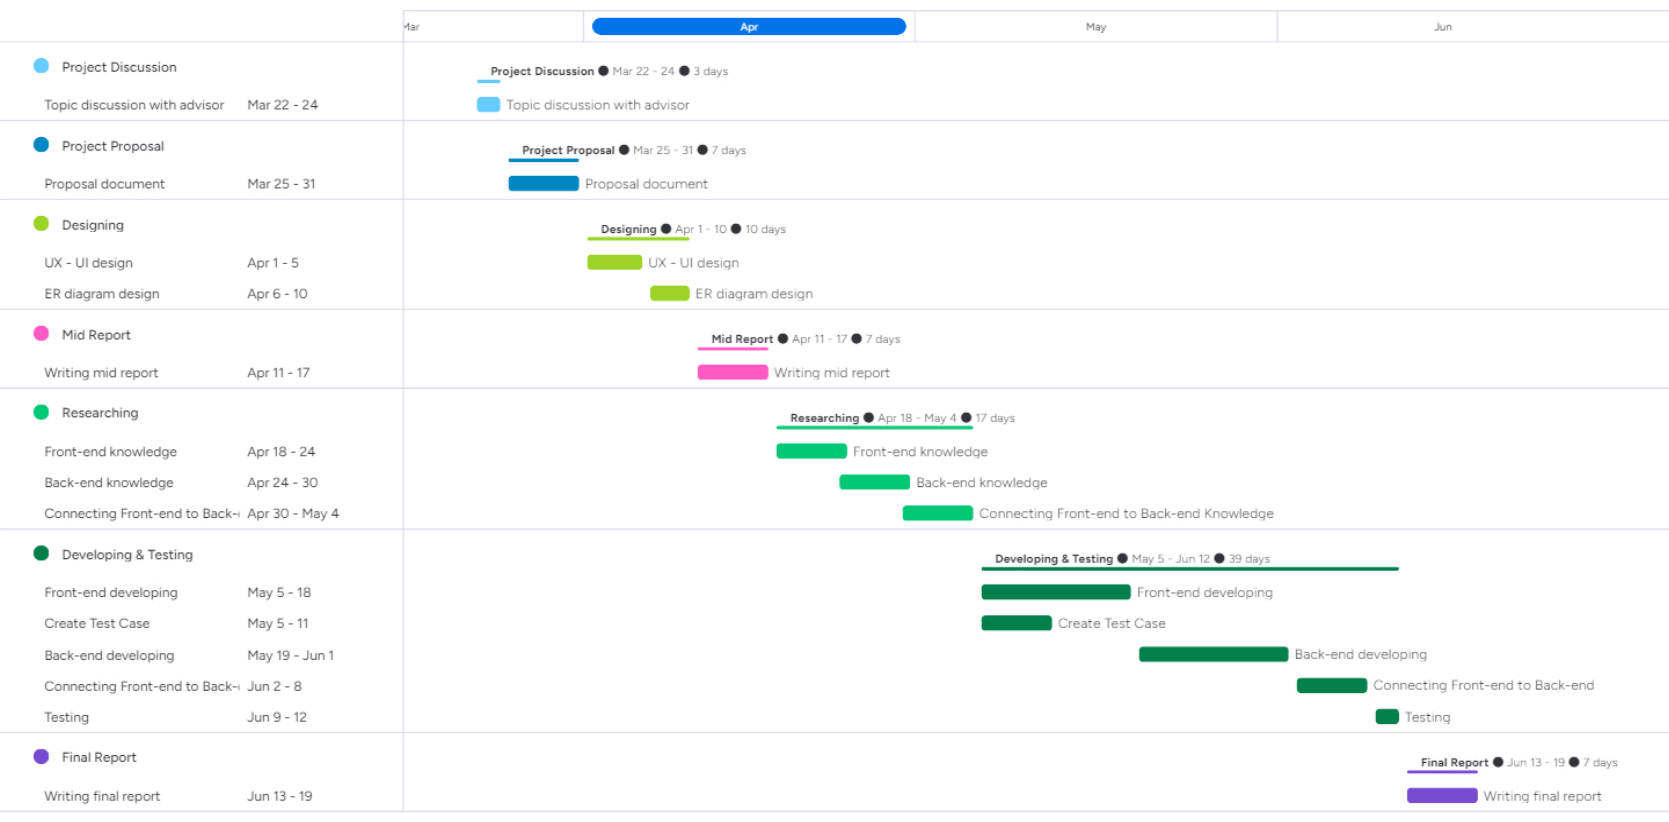
\includegraphics[width=\textwidth, keepaspectratio=true]{image/chap1/gantt.png}}
	\caption{ตารางการดำเนินงานภาคการศึกษาที่ 1}\label{fig:plan}
\end{figure}

\section{ผลการดำเนินงาน}

\begin{itemize}
	\item รายงานรูปเล่มฉบับสมบูรณ์
	\item การออกแบบ
	      \begin{itemize}
		      \item รายละเอียดของระบบ
		      \item โครงสร้างสถาปัตยกรรมระบบ
		      \item แบบจำลองหน้าจอส่วนต่อประสานกับผู้ใช้
		      \item โครงสร้างฐานข้อมูล
		      \item แผนภาพความสามารถของระบบ และแผนภาพการทำงานของระบบ
	      \end{itemize}
	\item ระบบ Front-end
	\item ระบบ Back-end
	\item ข้อมูลคำศัพท์ในฐานข้อมูลเริ่มต้นจำนวน 100 คำ ที่สามารถเพิ่มเติมได้ในภายหลัง
\end{itemize}

%%%%%%%%%%%%%%%%%%%%%%%%%%%%%%%%%%%%%%%%%%%%%%%%%%%%%%%%%%%%%%%
%%%%%%%%%%%%%%%%%%%%%%%%%% Chapter 2 %%%%%%%%%%%%%%%%%%%%%%%%%%
%%%%%%%%%%%%%%%%%%%%%%%%%%%%%%%%%%%%%%%%%%%%%%%%%%%%%%%%%%%%%%%

\chapter{ทฤษฎีและงานวิจัยที่เกี่ยวข้อง}

%%%%%%%%%%%%%%%%%%%%%%%%%% 2.1 %%%%%%%%%%%%%%%%%%%%%%%%%%

\section{ทฤษฎีที่เกี่ยวข้อง}

\hspace{1cm}
หัวข้อนี้จะพูดเกี่ยวกับทฤษฎีที่เกี่ยวข้องกับโครงงาน โดยหัวข้อที่เกี่ยวข้องคือวิธีการเรียนรู้คำศัพท์
คือการใช้บัตรคำในการจำศัพท์ และข้อสอบแบบเลือกตอบสำหรับการวัดผล และวิธีการเรียนรู้รูปแบบต่าง ๆ
ที่นำมาปรับใช้ในโครงงาน คือ Computer-Aided Instruction ซึ่งเป็นการนำคอมพิวเตอร์มาปรับใช้กับการเรียนรู้
และ Games-Based Learning ซึ่งเป็นการนำเกมมาใช้เป็นสื่อการสอน

\subsection{การเรียนรู้คำศัพท์}

\hspace{1cm}
การเรียนรู้คำศัพท์ \cite{LearnEng} คือ กระบวนการเรียนรู้คำศัพท์ โดยใช้ความรู้ ความจำ และความเข้าใจในความหมาย เมื่อเรียนรู้แล้วจะเข้าใจความหมายของคำ
การสะกด การออกเสียงของคำศัพท์ใหม่ ๆ อีกทั้งยังรวมถึงการนำคำศัพท์ที่เรียนรู้มาไปใช้ในบริบทต่าง ๆ ได้อย่างถูกต้อง

\subsection{บัตรคำ}

\hspace{1cm}
บัตรคำ (Flash card) \cite{Flashcard} เป็นสื่อการสอนในรูปแบบหนึ่ง โดยด้านหนึ่งจะประกอบไปด้วยคำศัพท์
และอีกด้านจะเป็นความหมายหรือรูปภาพของคำศัพท์นั้น ๆ อีกทั้งยังสามารถประยุกใช้ในการจำสิ่งต่าง ๆ ได้เพิ่มเติม เช่น
สูตรทางคณิตศาสตร์ และสูตรทางเคมี การใช้บัตรจำในการจำคำศัพท์นั้นใช้หลักการการทบทวนแบบเว้นระยะ [\ref{ssec:SpacedRepetition}]
ซึ่งจะช่วยกระตุ้นทักษะในด้านการจดจำคำศัพท์ให้ดียิ่งขึ้น

\subsection{การทบทวนแบบเว้นระยะ}\label{ssec:SpacedRepetition}

\hspace{1cm}
การทบทวนแบบเว้นระยะ \cite{SpacedRepetition} คือการทบทวนความจำของเราซ้ำอีกครั้งเมื่อผ่านไปแล้วเป็นระยะเวลาหนึ่ง ตามหลักการแล้วควรทบทวนทั้งหมด 4 ครั้ง คือ
1. หลังได้รับข้อมูล 2. 1 วันหลังได้รับข้อมูล 3. 1 สัปดาห์หลังได้รับข้อมูล 4. 1 เดือนหลังได้รับข้อมูล
ซึ่งจะเป็นการช่วยกระตุ้นสมองเพื่อเรียกใช้ความจำนั้น ๆ อยู่เสมอ และตามหลักการการทำงานของสมองแล้วแล้วความจำของเราจะลดลงตามเวลาที่ผ่านไป
แต่ถ้าหากใช้การทบทวนแบบเว้นระยะจะสามารถช่วยให้เราจำสิ่งนั้น ๆ ได้ดียิ่งขึ้น

\subsection{ข้อสอบแบบเลือกตอบ}

\hspace{1cm}
ข้อสอบแบบเลือกตอบ (Multiple choice question) \cite{MultiChoices} เป็นเครื่องมือการวัดผลชนิดหนึ่งที่มีลักษณะสำคัญคือ
เป็นคำถามและมีตัวเลือกหลายตัวเลือกให้ผู้สอบเลือกตอบข้อที่ถูกเพียงข้อเดียว จะใช้วัดผลด้านความรู้เป็นหลัก
มีข้อดีคือสามารถตรวจให้คะแนนได้เหมือนกันแม้จะเป็นผู้ตรวจคนละคนกัน อีกทั้งยังสามารถประเมินความรู้ได้ทั้งในระดับของความจำ
และการประยุกต์ใช้ความรู้ แต่ทั้งนี้ในการจะวัดความรู้ได้ดีหรือไม่ก็ขึ้นอยู่กับการสร้างคำถาม

\subsection{Games-Based Learning}

\hspace{1cm}
Games-based learning \cite{GBL} คือการเรียนรู้โดยใช้เกมมาผสมผสาน ซึ่งจะทำให้เกิดการเรียนรู้ไปพร้อมกับได้รับความสนุกจากเกม
โดยเกิดจากการที่นักวิจัยด้านการศึกษาได้นำเสนอแนวคิดที่จะนำความบันเทิงเข้ามาเป็นส่วนหนึ่งกับการเรียนรู้ และเมื่อการเรียนมีความสนุกสนาน
ก็จะช่วยให้ผู้เรียนมีความสนใจในการเรียนรู้มากขึ้น และทำให้เกิดการเรียนรู้ได้เร็วยิ่งขึ้น ต่างจากการเรียนปกติที่อาจทำให้เกิดความเคร่งเครียด
และนำไปสู่การไม่สนใจในการเรียนรู้ และละเลยการศึกษา

\subsection{Computer-Aided Instruction}

\hspace{1cm}
Computer-Aided Instruction \cite{CAI1,CAI2} คือสื่อการเรียนรู้รูปแบบหนึ่ง ที่ใช้ความสามารถของคอมพิวเตอร์นำเสนอสื่อ และข้อมูลต่าง ๆ
ไม่ว่าจะเป็นข้อความ ภาพ หรือเสียง โดยมีลักษณะการเรียนแบบที่ผู้เรียนมีการโต้ตอบโดยตรงกับคอมพิวเตอร์
ซึ่งจะช่วยดึงดูดความสนใจของผู้เรียน และสร้างแรงจูงใจในการเรียนรู้มากขึ้น

%%%%%%%%%%%%%%%%%%%%%%%%%% 2.2 %%%%%%%%%%%%%%%%%%%%%%%%%%

\pagebreak
\section{ภาษาคอมพิวเตอร์และเทคโนโลยี}

\hspace{1cm}
หัวข้อนี้จะพูดถึงภาษาคอมพิวเตอร์และเทคโนโลยีที่ใช้ในโครงงาน ประกอบไปด้วย Figma ใช้ออกแบบ User Interface,
React
และ Tailwind CSS
ซึ่งใช้พัฒนา Frontend และ Django ที่ใช้พัฒนา Backend

\subsection{Figma}

\hspace{1cm}
Figma \cite{Figma} เป็นเครื่องมือออกแบบกราฟิกแบบออนไลน์ที่ช่วยให้นักออกแบบสามารถสร้างและออกแบบ UI/UX ของเว็บไซต์
แอปพลิเคชั่น หรือผลิตภัณฑ์อื่น ๆ ได้อย่างง่ายดาย และมีความยืดหยุ่นสูง สามารถใช้งานได้ทั้งบนเว็บและอุปกรณ์เคลื่อนที่
อีกทั้ง Figma ยังได้อันดับ 1 ในการจัดอันดับ UI design tool ประจำปี 2022 ของ uxtool.co อีกด้วย

\subsection{React}

\hspace{1cm}
React \cite{React} เป็น JavaScript Library สำหรับการสร้าง User interface โดยมีความสามารถในการแบ่ง UI ที่มีความซับซ้อนให้เป็น Component หรือส่วนเล็ก ๆ
แต่ละส่วนสามารถแยกการทำงานได้อย่างอิสระ และสามารถนำแต่ละส่วนกลับมาใช้ได้อีก ซึ่งทำให้ง่ายต่อการจัดการและแก้ไขโค้ด

\subsection{Tailwind CSS}

\hspace{1cm}
Tailwind CSS \cite{Tailwind} คือ CSS framework ที่เป็นรูปแบบ "utility-first" ซึ่งทำให้สามารถพัฒนา UI อย่างรวดเร็วและสะดวกมากยิ่งขึ้น
โดยทั่วไปแล้ว CSS framework เป็นชุดของ Class CSS สำเร็จรูปที่สามารถเรียกใช้ได้เลย แต่ Tailwind CSS สามารถเรียกใช้ Utility มาประกอบกัน
ผ่าน Class ของ Element นั้น เพื่อให้แสดงผลได้ตามต้องการได้เลย

\subsection{Django}

\hspace{1cm}
Django \cite{Django} เป็น Web framework สำหรับการสร้างเว็บแอปพลิเคชันโดยใช้ภาษา Python ซึ่งมี Architectural pattern
แบบ Model-View-Controller (MVC) และมีคุณสมบัติหลากหลาย เช่น มีระบบแอดมินที่สามารถใช้งานได้ทันที
มี Object-Relational Mapping (ORM) ที่ช่วยให้เชื่อมต่อกับฐานข้อมูลได้อย่างสะดวก และระบบการยืนยันตัวตน (Authentication)
ซึ่งทำให้ง่ายต่อการพัฒนาและปรับปรุงเว็บไซต์ที่ซับซ้อนได้อย่างรวดเร็ว



%%%%%%%%%%%%%%%%%%%%%%%%%% 2.3 %%%%%%%%%%%%%%%%%%%%%%%%%%
\pagebreak
\section{งานวิจัยที่เกี่ยวข้อง}

\hspace{1cm}
หัวข้อนี้จะพูดถึงงานวิจัยที่เกี่ยวข้อกับโครงงาน โดยจะเป็นแอปพลิเคชันที่เกี่ยวข้องกับการเรียนภาษาอังกฤษ
ประกอบไปด้วย Duocards, Memrise และ Duolingo

\begin{table}[h]\centering
	\caption{ตารางสรุปคุณสมบัติของงานวิจัยที่เกี่ยวข้อง}\label{tbl:RelatedResearch}
	\begin{tabular}{|c|ccccccc|l|}
		\hline
		\multirow{2}{*}{แอปพลิเคชัน}                                & \multicolumn{7}{c|}{คุณสมบัติ}                                                     & \multicolumn{1}{c|}{\multirow{2}{*}{ข้อเสีย}}                                                                                                                                                                                                                                                                                                                         \\ \cline{2-8}
		                                                          & \multicolumn{1}{c|}{\begin{tabular}[c]{@{}c@{}}การเรียน\\ หลายภาษา\end{tabular}} & \multicolumn{1}{c|}{สร้างบทเรียน}             & \multicolumn{1}{c|}{\begin{tabular}[c]{@{}c@{}}การเรียนรู้\\ รูปแบบเกม\end{tabular}} & \multicolumn{1}{c|}{ชุมชนผู้ใช้}  & \multicolumn{1}{c|}{บัตรคำ}     & \multicolumn{1}{c|}{\begin{tabular}[c]{@{}c@{}}ข้อสอบ\\ แบบเลือกตอบ\end{tabular}} & เกม      & \multicolumn{1}{c|}{}                                                 \\ \hline
		Duocards                                                  & \multicolumn{1}{c|}{\faCheck}                                                   & \multicolumn{1}{c|}{\faCheck}               & \multicolumn{1}{c|}{\faCheck}                                                    & \multicolumn{1}{c|}{\faCheck} & \multicolumn{1}{c|}{\faCheck} & \multicolumn{1}{c|}{}                                                           &          & - มีเฉพาะบัตรคำ                                                          \\ \hline
		Memrise                                                   & \multicolumn{1}{c|}{\faCheck}                                                   & \multicolumn{1}{c|}{\faCheck}               & \multicolumn{1}{c|}{\faCheck}                                                    & \multicolumn{1}{c|}{\faCheck} & \multicolumn{1}{c|}{}         & \multicolumn{1}{c|}{\faCheck}                                                   &          & \begin{tabular}[c]{@{}l@{}}- ไม่สามารถเลือก\\ รูปแบบการเรียน\end{tabular} \\ \hline
		Duolingo                                                  & \multicolumn{1}{c|}{\faCheck}                                                   & \multicolumn{1}{c|}{}                       & \multicolumn{1}{c|}{\faCheck}                                                    & \multicolumn{1}{c|}{\faCheck} & \multicolumn{1}{c|}{}         & \multicolumn{1}{c|}{\faCheck}                                                   &          & \begin{tabular}[c]{@{}l@{}}- ไม่เหมาะสำหรับ\\ การเรียนศัพท์\end{tabular}    \\ \hline
		\begin{tabular}[c]{@{}c@{}}แอปพลิชัน\\ ของผู้จัดทำ\end{tabular} & \multicolumn{1}{c|}{}                                                           & \multicolumn{1}{c|}{\faCheck}               & \multicolumn{1}{c|}{\faCheck}                                                    & \multicolumn{1}{c|}{}         & \multicolumn{1}{c|}{\faCheck} & \multicolumn{1}{c|}{\faCheck}                                                   & \faCheck & - มีเฉพาะภาษาอังกฤษ                                                     \\ \hline
	\end{tabular}
\end{table}

\pagebreak
\subsection{DuoCards}

\hspace{1cm}
DuoCards  \cite{DuoCards} เป็นแอปพลิชันที่ออกแบบมาเพื่อช่วยให้ผู้ใช้สามารถเรียนรู้และจดจำคำศัพท์ ใหม่ ๆ ในหลายภาษาโดยใช้บัตรคำ
โดยผู้ใช้สามารถใช้ชุดคำศัพท์ที่มีการเตรียมไว้ให้ หรือสร้างและออกแบบบัตรคำของตัวเองได้

\begin{figure}[!h]\centering
	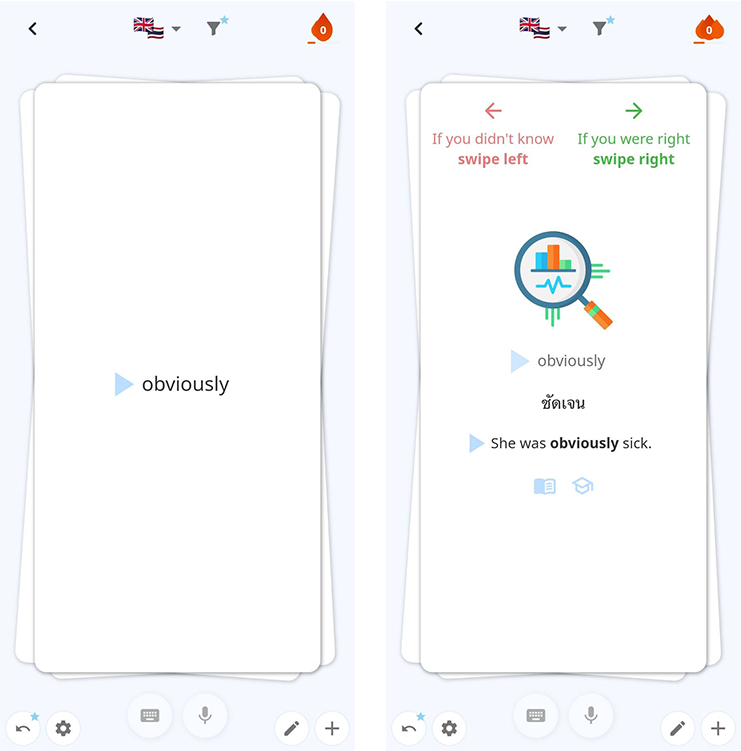
\includegraphics[width=0.8\textwidth, keepaspectratio=true]{image/chap2/duocardsEX.png}
	\caption[แอปพลิเคชัน Duocards]{แอปพลิเคชัน Duocards\\ (ที่มา: \href {https://play.google.com/store/apps/details?id=com.duocards.app} {https://play.google.com/store/apps/details?id=com.duocards.app})\centering}\label{fig:duocardsEx}
\end{figure}

\begin{itemize}
	\item ข้อดี
	      \begin{enumerate}
		      \item มีคอร์สเรียนและแบบฝึกหัดในหลากหลายภาษา
		      \item สามารถสร้างชุดคำศัพท์ของตัวเองได้
		      \item สามารถเรียนรู้คำศัพท์จากวิดีโอที่แอปพลิเคชันเตรียมไว้ให้ได้
		      \item มีการเรียนรู้ในรูปแบบเกมที่มีรางวัลและความสำเร็จเพื่อเป็นแรงจูงใจให้ผู้ใช้
		      \item มีชุมชนสำหรับผู้ใช้เพื่อการแข่งขันและแลกเปลี่ยนข้อมูล
	      \end{enumerate}
	\item ข้อเสีย
	      \begin{enumerate}
		      \item มีวิธีการเรียนรู้คำศัพท์ในรูปแบบเดียวเท่านั้นคือบัตรคำ
	      \end{enumerate}
\end{itemize}

\pagebreak
\subsection{Memrise}

\hspace{1cm}
Memrise \cite{Memrise} เป็นแอปพลิเคชันสำหรับการเรียนรู้ภาษาที่มีรูปแบบในการเรียนรู้หลากหลาย ไม่ว่าจะเป็นแบบทดสอบหลายตัวเลือก
หรือการพิมพ์คำศัพท์ให้ถูกต้อง อีกทั้งยังมีภาษาให้เลือกเรียนถึง 22 ภาษา โดยผู้ใช้สามารถสร้างบทเรียนของตัวเองเพื่อแบ่งปันกับผู้ใช้คนอื่นได้อีกด้วย

\begin{figure}[!h]\centering
	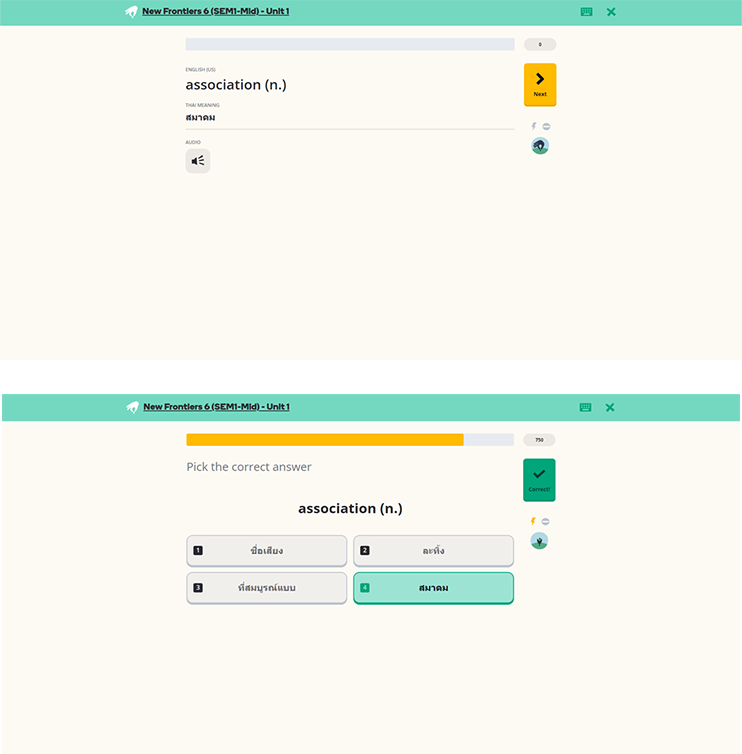
\includegraphics[width=0.8\textwidth, keepaspectratio=true]{image/chap2/memriseEX.png}
	\caption[แอปพลิเคชัน Memrise]{แอปพลิเคชัน Memrise \\ (ที่มา: \href {https://app.memrise.com} {https://app.memrise.com})\centering}\label{fig:mimriseEx}
\end{figure}

\begin{itemize}
	\item ข้อดี
	      \begin{enumerate}
		      \item มีคอร์สเรียนและแบบฝึกหัดในหลายภาษา และยังสามารถเลือกหัวข้อการเรียนที่สนใจได้ เช่นคำศัพท์ทางวิทยาศาสตร์ หรือคำศัพท์ทางธุรกิจ
		      \item สามารถสร้างบทเรียนหรือชุดคำศัพท์ของตนเองเพื่อแบ่งปันกับผู้ใช้งานคนอื่นได้
		      \item มีการเก็บค่าประสบการณ์ และความสำเร็จเพื่อเป็นแรงจูงใจให้ผู้ใช้
		      \item มีชุมชนสำหรับผู้ใช้เพื่อการแข่งขันและแลกเปลี่ยนข้อมูล
	      \end{enumerate}
	\item ข้อเสีย
	      \begin{enumerate}
		      \item การเรียนรู้ส่วนใหญ่ที่มีจะอยู่ในรูปแบบการเลือกคำตอบให้ถูกต้อง
		      \item ไม่สามารถเลือกรูปแบบการเรียนรู้ของบทเรียนที่มีอยู่ ยกเว้นจะทำการสร้างบทเรียนขึ้นมาเอง
	      \end{enumerate}
\end{itemize}

\pagebreak
\subsection{Duolingo}

\hspace{1cm}
Duolingo \cite{Duolingo} เป็นแอปพลิเคชันสำหรับการเรียนรู้ภาษาที่ครอบคลุมถึง 40 ภาษา อีกทั้งยังมีการเรียนรู้ที่ครอบคลุมทั้งการฟัง การพูด การอ่าน และการเขียน
ตัวอย่างเช่นการจับคู่คำศัพท์, แบบทดสอบหลายตัวเลือก, การเรียงประโยคให้ถูกต้อง และการฝึกพูด เป็นต้น ซึ่งทำให้การเรียนรู้มีความสนุกและน่าสนใจมากขึ้น

\begin{figure}[!h]\centering
	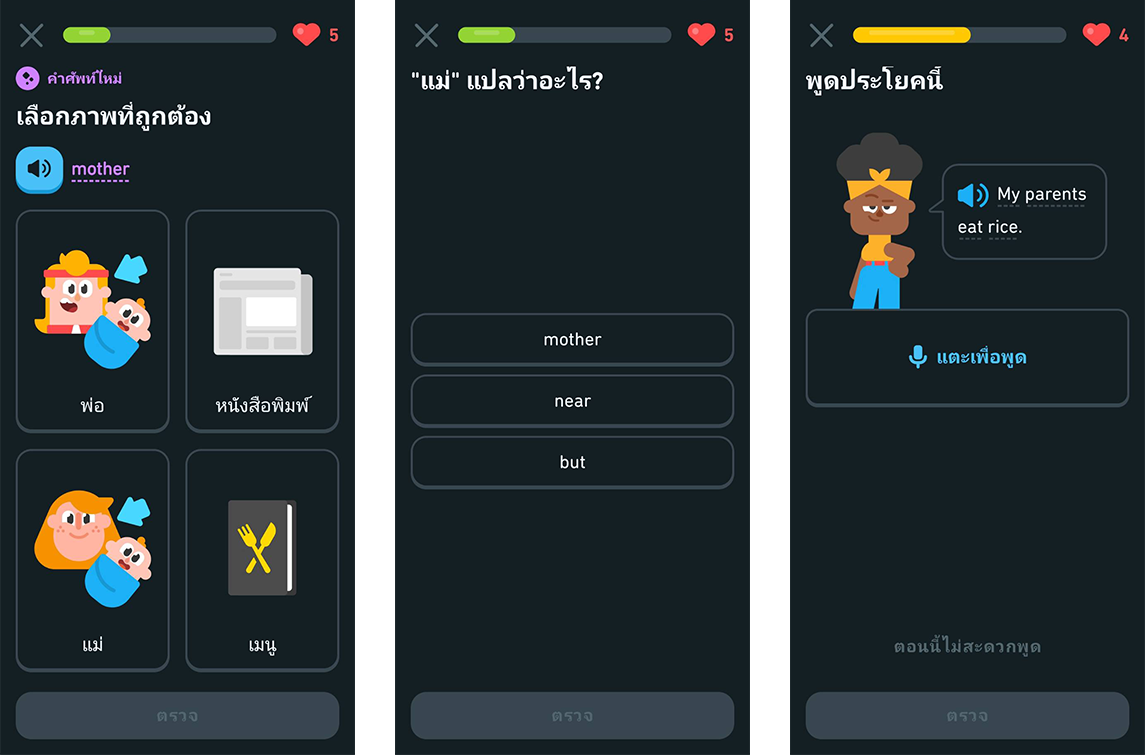
\includegraphics[width=0.8\textwidth, keepaspectratio=true]{image/chap2/duolingoEX.png}
	\caption[แอปพลิเคชัน Duolingo]{แอปพลิเคชัน Duolingo \\ (ที่มา: \href {https://play.google.com/store/apps/details?id=com.duolingo} {https://play.google.com/store/apps/details?id=com.duolingo})\centering}\label{fig:duolingoEX}
\end{figure}

\begin{itemize}
	\item ข้อดี
	      \begin{enumerate}
		      \item มีคอร์สเรียนและแบบฝึกหัดในหลายภาษา
		      \item มีระบบการเรียนรู้ที่หลากหลาย ทั้งฟัง พูด อ่าน และเขียนสามารถสร้างบทเรียนหรือชุดคำศัพท์ของตนเองเพื่อแบ่งปันกับผู้ใช้งานคนอื่นได้
		      \item มีระบบการเรียนรู้แบบเกมที่มีรางวัลและความสำเร็จที่สามารถให้แรงจูงใจกับผู้ใช้ได้
		      \item มีชุมชนสำหรับผู้ใช้เพื่อการแข่งขันและแลกเปลี่ยนข้อมูล
	      \end{enumerate}
	\item ข้อเสีย
	      \begin{enumerate}
		      \item แอปอาจไม่เหมาะสำหรับผู้ใช้ที่ต้องการเน้นการเรียนรู้คำศัพท์เท่านั้น เนื่องจากแอปถูกออกแบบให้เป็นแพลตฟอร์มการเรียนรู้ภาษาแบบครอบคลุม
		      \item ไม่สามารถเลือกหมวดหมู่ของการเรียนได้ตามต้องการ ต้องเรียนตามบทเรียนที่แอปพลิเคชันสร้างไว้
		      \item ไม่สามารถสร้างบทเรียนของตนเองได้
	      \end{enumerate}
\end{itemize}

%%%%%%%%%%%%%%%%%%%%%%%%%%%%%%%%%%%%%%%%%%%%%%%%%%%%%%%%%%%%%%%
%%%%%%%%%%%%%%%%%%%%%%%%%% Chapter 3 %%%%%%%%%%%%%%%%%%%%%%%%%%
%%%%%%%%%%%%%%%%%%%%%%%%%%%%%%%%%%%%%%%%%%%%%%%%%%%%%%%%%%%%%%%

\chapter{การออกแบบและวิธีดำเนินงาน}

\section{รายละเอียดของโครงงาน}
\hspace{1cm}
หัวข้อนี้จะพูดถึงรายละเอียดต่าง ๆ ที่โครงงานสามารถทำได้ โดยจะประกอบไปด้วยความต้องการระบบ
ซึ่งเป็นความต้องการพื้นฐาน และคุณสมบัติต่าง ๆ ของระบบ รวมถึง Use Case Diagram
และ Use Case Narrative ซึ่งจะแสดงให้เห็นถึงสิ่งที่ระบบสามารถทำได้

\subsection{ความต้องการระบบ}
\begin{itemize}
	\item สามารถเข้าถึงได้ผ่านทุกเว็บเบราเซอร์บนคอมพิวเตอร์
	\item ฐานข้อมูลคำศัพท์โดยเป็นคำศัพท์ภาษาอังกฤษที่สามารถค้นหาได้ พร้อมความหมายทั้งภาษาไทยและภาษาอังกฤษ ตัวอย่างการใช้งานในประโยค และวิธีการออกเสียง
	\item สามารถสุ่มคำศัพท์ภาษาอังกฤษใหม่ ๆ ที่ยังไม่เคยเรียน พร้อมความหมายทั้งภาษาไทย ภาษาอังกฤษ ตัวอย่างการใช้งานในประโยค และวิธีการออกเสียง
	\item สามารถใช้งานบัตรคำ ซึ่งเป็นบัตรที่ประกอบไปด้วยคำศัพท์ภาษาอังกฤษ และความหมายภาษาไทยได้
	\item สามารถทดสอบความรู้ด้วยแบบทดสอบหลายตัวเลือกได้ โดยผู้ใช้จะต้องทำการจับคู่คำศัพท์กับความหมายให้ถูกต้อง
	\item สามารถเล่นเกมเรียงพยัญชนะเป็นคำศัพท์ได้ โดยระบบจะทำการสลับตำแหน่งตัวอักษร และให้คำใบ้มา ผู้ใช้จะต้องทำการพิมพ์คำศัพท์ที่ถูกต้อง
	\item สามารถติดตามความคืบหน้าได้ โดยมีคำศัพท์และจำนวนคำศัพท์ที่เรียนไป จำนวนเกมที่เล่นจบ คะแนนของแบบทดสอบ คะแนนรวม และเวลาที่ใช้ไปในแอปพลิเคชัน
	\item สามารถเก็บคะแนนที่ได้จากการทำแบบทดสอบและเกมไว้ในระบบ และสามารถวัดคะแนนกับผู้เล่นคนอื่นได้
\end{itemize}

\pagebreak
\subsection{Use Case Diagram}

\begin{figure}[!h]\centering
	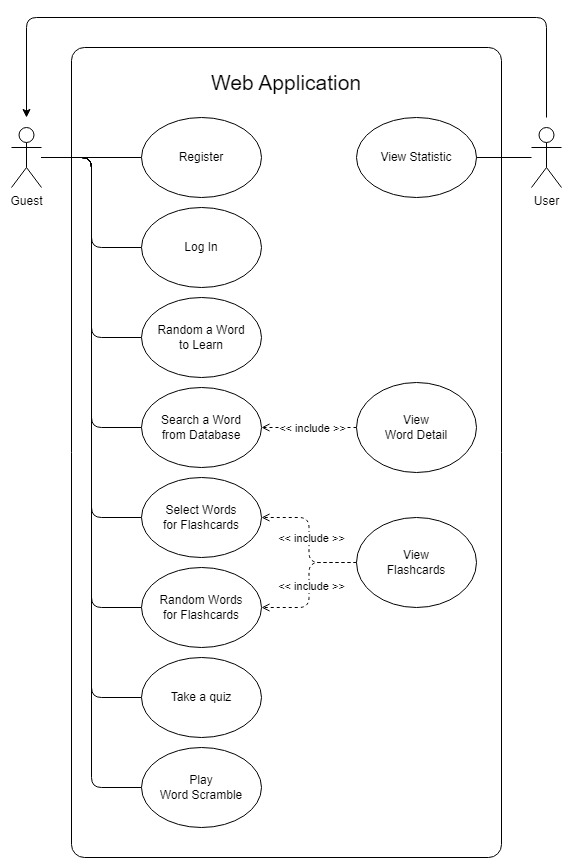
\includegraphics[width=0.8\textwidth, keepaspectratio=true]{image/chap3/UseCaseDiagram.jpg}
	\caption{แผนภาพที่แสดงการทำงานของระบบ}\label{fig:UseCaseDiagram}
\end{figure}

\hspace{1cm}
จากรูปภาพที่ \ref{fig:UseCaseDiagram} จะเห็นว่าประกอบด้วย 2 บทบาทคือ Guest และ User โดยแต่ละบทบาทมีหน้าที่ดังนี้
\begin{itemize}
	\item Guest คือผู้ใช้ทั่วไปที่ยังไม่ได้ลงทะเบียนผู้ใช้ในระบบ หรือยังไม่ได้เข้าสู่ระบบ
	      โดยสามารถลงทะเบียนผู้ใช้งาน เข้าสู่ระบบ สุ่มคำศัพท์ ค้นหาคำศัพท์ แสดงรายละเอียดคำศัพท์ที่ค้นหา
	      สุ่มคำศัพท์เพื่อใช้งานบัตรคำ ดูบัตรคำ ทำแบบทดสอบ และเล่นเกม
	\item User คือผู้ใช้ที่เข้าสู่ระบบแล้ว สามารถดูสถิติการใช้งานเว็บแอปพลิชัน ดูคำศัพท์ที่เคยเรียน และดูกระดานผู้นำได้
\end{itemize}

\subsection{Use Case Narrative}
ประกอบด้วย 12 Use Cases ดังรูปภาพที่ \ref{fig:UseCaseDiagram} โดยมีรายละเอียดดังนี้

\subsubsection{ลงทะเบียนผู้ใช้งาน}
\hspace{1cm}
การลงทะเบียนผู้ใช้งาน Guest ที่อยู่หน้า Register/Log In จะทำการกรอกข้อมูลและทำการยืนยันข้อมูลเพื่อให้ระบบทำการสร้างบัญชีผู้ใช้ใหม่ให้ ดังตารางที่ \ref{tbl:U_Register}
\begin{table}[h]\centering
	\caption{คำอธิบาย Use Case สำหรับการลงทะเบียนผู้ใช้งาน}\label{tbl:U_Register}
	\begin{tabular}{|p{.2\linewidth}|p{.6\linewidth}|}
		\hline
		Use Case Name:         & Register                                                                                                                                    \\ \hline
		Actor:                 & Guest                                                                                                                                       \\ \hline
		Goal:                  & ลงทะเบียนผู้ใช้งานสำเร็จ                                                                                                                          \\ \hline
		Precondition           & Guest เข้าหน้า Register/Log In                                                                                                                \\ \hline
		Main Success Scenario: & \begin{tabular}[c]{@{}l@{}}1. ระบบร้องขอการกรอกข้อมูล \\2. Guest กรอกข้อมูล \\3. Guest ยืนยันข้อมูล \\4. ระบบสร้างบัญชีผู้ใช้ให้กับ Guest\end{tabular}       \\ \hline
		Postcondition          & Guest มีบัญชีในระบบ                                                                                                                            \\ \hline
		Extention              & \begin{tabular}[c]{@{}l@{}}Extension (a) \\ 3a. ข้อมูลที่ Actor กรอกมาซ้ำกับที่มีอยู่ในระบบ \\ 4a. ระบบแจ้งเตือนข้อผิดพลาด \\ 5a. กลับไปทำข้อ 1. \end{tabular} \\ \hline
	\end{tabular}
\end{table}

\subsubsection{เข้าสู่ระบบ}
\hspace{1cm}
การเข้าสู่ระบบ Guest ต้องมีบัญชีผู้ใช้และอยู่ที่หน้า Register/Log In จากนั้นก็กรอกข้อมูลผู้ใช้ เพื่อให้ระบบตรวจสอบและอนุญาตให้การเข้าสู่ระบบ ดังตารางที่ \ref{tbl:U_LogIn}
\begin{table}[h]\centering
	\caption{คำอธิบาย Use Case สำหรับการเข้าสู่ระบบ}\label{tbl:U_LogIn}
	\begin{tabular}{|p{.2\linewidth}|p{.6\linewidth}|}
		\hline
		Use Case Name:         & Log In                                                                                                                               \\ \hline
		Actor:                 & Guest                                                                                                                                \\ \hline
		Goal:                  & เข้าสู่ระบบสำเร็จ                                                                                                                         \\ \hline
		Precondition           & Guest เข้าหน้า Register/Log In และ Guest มีบัญชีผู้ใช้งานในระบบ                                                                              \\ \hline
		Main Success Scenario: & \begin{tabular}[c]{@{}l@{}}1. Actor กรอก Username และ Password \\2. Actor กดยืนยัน \\3. ระบบยืนยันให้เข้าสู่ระบบ \end{tabular}               \\ \hline
		Extention              & \begin{tabular}[c]{@{}l@{}}Extension (a) \\ 3a. ข้อมูลที่ Actor กรอกมาไม่ถูกต้อง \\ 4a. ระบบแจ้งเตือนข้อผิดพลาด \\ 5a. กลับไปทำข้อ 1.\end{tabular} \\ \hline
	\end{tabular}
\end{table}

\pagebreak
\subsubsection{ดูสถิติการใช้งานเว็บแอปพลิเคชัน}
\hspace{1cm}
เมื่อเข้าสู่ระบบแล้ว User จะสามารถกดปุ่มดูสถิติ เพื่อให้ระบบแสดงผลสถิติการใช้งานเว็บแอปพลิเคชันได้ ดังตารางที่ \ref{tbl:U_Statistic}
\begin{table}[h]\centering
	\caption{คำอธิบาย Use Case สำหรับการดูสถิติการใช้งานเว็บแอปพลิเคชัน}\label{tbl:U_Statistic}
	\begin{tabular}{|p{.2\linewidth}|p{.6\linewidth}|}
		\hline
		Use Case Name:         & View Statistic                                                                                 \\ \hline
		Actor:                 & User                                                                                           \\ \hline
		Goal:                  & แสดงสถิติการใช้งานเว็บแอปพลิเคชันสำเร็จ                                                                \\ \hline
		Precondition           & User ทำการ Log-in เข้ามาแล้ว และ User กดที่ไอคอนผู้ใช้งาน                                              \\ \hline
		Main Success Scenario: & \begin{tabular}[c]{@{}l@{}}1. User เลือกดูสถิติ \\2. ระบบแสดงสถิติการใช้งานเว็บแอปพลิเคชัน \end{tabular} \\ \hline
	\end{tabular}
\end{table}

\subsubsection{ดูคำศัพท์ที่เคยเรียน}
\hspace{1cm}
เมื่อเข้าสู่ระบบแล้ว User จะสามารถกดปุ่มดูคำศัพท์ที่เคยเรียน เพื่อให้ระบบแสดงผลคำศัพท์ที่เคยเรียนได้ ดังตารางที่ \ref{tbl:U_WordsLearned}
\begin{table}[h]\centering
	\caption{คำอธิบาย Use Case สำหรับการดูคำศัพท์ที่เคยเรียน}\label{tbl:U_WordsLearned}
	\begin{tabular}{|p{.2\linewidth}|p{.6\linewidth}|}
		\hline
		Use Case Name:         & View Words Learned                                                                           \\ \hline
		Actor:                 & User                                                                                         \\ \hline
		Goal:                  & แสดงคำศัพท์ที่เคยเรียนได้สำเร็จ                                                                       \\ \hline
		Precondition           & User อยู่หน้าแสดงผลสถิติ                                                                          \\ \hline
		Main Success Scenario: & \begin{tabular}[c]{@{}l@{}}1. User กดปุ่มดูคำศัพท์ที่เคยเรียน \\2. ระบบแสดงคำศัพท์ที่เคยเรียน \end{tabular} \\ \hline
	\end{tabular}
\end{table}

\subsubsection{ดูกระดานผู้นำ}
\hspace{1cm}
เมื่อเข้าสู่ระบบแล้ว User จะสามารถกดปุ่มดูกระดานผู้นำ เพื่อให้ระบบแสดงผลกระดานผู้นำได้ ดังตารางที่ \ref{tbl:U_Leaderboard}
\begin{table}[h]\centering
	\caption{คำอธิบาย Use Case สำหรับการดูกระดานผู้นำ}\label{tbl:U_Leaderboard}
	\begin{tabular}{|p{.2\linewidth}|p{.6\linewidth}|}
		\hline
		Use Case Name:         & View Leaderboard                                                                     \\ \hline
		Actor:                 & User                                                                                 \\ \hline
		Goal:                  & แสดงกระดานผู้นำสำเร็จ                                                                     \\ \hline
		Precondition           & User ทำการ Log-in เข้ามาแล้ว และ User กดที่ไอคอนผู้ใช้งาน                                    \\ \hline
		Main Success Scenario: & \begin{tabular}[c]{@{}l@{}}1. User เลือกดูกระดานผู้นำ \\2. ระบบแสดงกระดานผู้นำ \end{tabular} \\ \hline
	\end{tabular}
\end{table}

\pagebreak
\subsubsection{สุ่มคำศัพท์ใหม่เพื่อการเรียนรู้}
\hspace{1cm}
Actor สามารถให้ระบบทำการสุ่มคำศัพท์ใหม่มาได้ผ่านปุ่ม Random Word ดังตารางที่ \ref{tbl:U_RandomWord}
\begin{table}[h]\centering
	\caption{คำอธิบาย Use Case สำหรับการสุ่มคำศัพท์ใหม่เพื่อการเรียนรู้}\label{tbl:U_RandomWord}
	\begin{tabular}{|p{.2\linewidth}|p{.6\linewidth}|}
		\hline
		Use Case Name:         & Random a Word to Learn                                                                    \\ \hline
		Actor:                 & Guest, User                                                                               \\ \hline
		Goal:                  & แสดงคำศัพท์ที่สุ่มมาสำเร็จ                                                                         \\ \hline
		Precondition           & Actor อยู่หน้า Homepage                                                                      \\ \hline
		Main Success Scenario: & \begin{tabular}[c]{@{}l@{}}1. Actor เลือก Random Word \\2. ระบบแสดงคำศัพท์ที่สุ่มมา \end{tabular} \\ \hline
	\end{tabular}
\end{table}

\subsubsection{ค้นหาคำศัพท์จากฐานข้อมูล}
\hspace{1cm}
การค้นหาคำศัพท์ในฐานข้อมูลสามารถทำได้ทุกที่ ที่ม่ช่องค้นหาคำศััพท์ เมื่อค้นหาแล้ว ระบบจะแสดงคำศัพท์ที่ตรงกับคำค้นหาออกมา ดังตารางที่ \ref{tbl:U_SearchWord}
\begin{table}[h]\centering
	\caption{คำอธิบาย Use Case สำหรับการค้นหาคำศัพท์จากฐานข้อมูล}\label{tbl:U_SearchWord}
	\begin{tabular}{|p{.2\linewidth}|p{.6\linewidth}|}
		\hline
		Use Case Name:         & Search a Word from Database                                                                                                      \\ \hline
		Actor:                 & Guest, User                                                                                                                      \\ \hline
		Goal:                  & แสดงคำศัพท์ที่ค้นหาสำเร็จ                                                                                                                \\ \hline
		Precondition           & Actor อยู่หน้าที่มีช่องค้นหา                                                                                                             \\ \hline
		Main Success Scenario: & \begin{tabular}[c]{@{}l@{}}1. Actor กรอกคำศัพท์ที่ต้องการค้นหา \\2. Actor กดค้นหา \\3. ระบบแสดงคำศัพท์ที่ค้นหา \end{tabular}                   \\ \hline
		Extention              & \begin{tabular}[c]{@{}l@{}}Extension (a) \\ 3a. ระบบไม่มีคำศัพท์ที่ Actor ค้นหา \\ 4a. ระบบแสดงว่าไม่มีคำศัพท์ \\ 5a. กลับไปทำข้อ 1.\end{tabular} \\ \hline
	\end{tabular}
\end{table}

\subsubsection{แสดงผลรายละเอียดคำศัพท์}
\hspace{1cm}
เมื่อระบบแสดงคำศัพท์ที่ตรงกับคำค้นหาออกมาแล้ว  Actor สามารถกดปุ่มเพื่อดูรายละเอียดเพิ่มเติมของคำศัพท์ได้ ดังตารางที่ \ref{tbl:U_WordDetail}
\begin{table}[h]\centering
	\caption{คำอธิบาย Use Case สำหรับการแสดงผลรายละเอียดคำศัพท์}\label{tbl:U_WordDetail}
	\begin{tabular}{|p{.2\linewidth}|p{.6\linewidth}|}
		\hline
		Use Case Name:         & View Word Detail                                                                                  \\ \hline
		Actor:                 & Guest, User                                                                                       \\ \hline
		Goal:                  & แสดงผลรายละเอียดคำศัพท์สำเร็จ                                                                           \\ \hline
		Precondition           & Actor ค้นหาคำศัพท์                                                                                    \\ \hline
		Main Success Scenario: & \begin{tabular}[c]{@{}l@{}}1. Actor กดปุ่มดูรายละเอียดคำศัพท์ \\2. ระบบแสดงผลรายละเอียดคำศัพท์ \end{tabular} \\ \hline
	\end{tabular}
\end{table}

% \subsubsection{เลือกคำศัพท์เพื่อใช้งานบัตรคำ}
% \hspace{1cm}
% Actor สามารถเลือกคำมาเพื่อใช้งานบัตรคำได้ โดยจะสามารถเลือกได้ทั้งหมด 10 คำ ต่อการใช้บัตรคำ 1 ครั้ง ดังตารางที่ \ref{tbl:U_RandomFlashCard} 
% \begin{table}[h]\centering
% 	\caption{คำอธิบาย Use Case สำหรับการเลือกคำศัพท์เพื่อใช้งานบัตรคำ}\label{tbl:U_RandomFlashCard}
% 	\begin{tabular}{|p{.2\linewidth}|p{.6\linewidth}|}
% 		\hline
% 		Use Case Name:         & Select Words for Flashcards                                                                                                                                 \\ \hline
% 		Actor:                 & Guest, User                                                                                                                                                 \\ \hline
% 		Goal:                  & Actor เลือกคำศัพท์สำเร็จ                                                                                                                                                \\ \hline
% 		Precondition           & Actor เลือก Select Word ในหน้า Flashcard                                                                                                                      \\ \hline
% 		Main Success Scenario: & \begin{tabular}[c]{@{}l@{}}1. ระบบแสดงคำศัพท์ \\2. Actor เลือกเก็บคำศัพท์นั้นเพื่อใช้งานบัตรคำ \\3. ระบบเก็บคำศัพท์ที่เลือก \\4. กลับไปทำข้อที่ 1. จนระบบเก็บคำศัพท์ครบ 10 คำ \end{tabular} \\ \hline
% 		Postcondition          & ระบบมีคำศัพท์เพื่อใช้แสดงบัตรคำ                                                                                                                                      \\ \hline
% 		Extention              & \begin{tabular}[c]{@{}l@{}}Extension (a) \\ 2a. Actor เลือกทิ้งคำศัพท์ \\ 3a. กลับไปทำข้อ 1. จนระบบเก็บคำศัพท์ครบ 10 คำ\end{tabular}                                      \\ \hline
% 	\end{tabular}
% \end{table}

\pagebreak
\subsubsection{สุ่มคำศัพท์เพื่อใช้งานบัตรคำ}
\hspace{1cm}
Actor สามารถให้ระบบทำการสุ่มคำศัพท์จำนวน 5 คำมาเพื่อใช้บัตรคำได้ ดังตารางที่ \ref{tbl:U_SelectFlashcard}
\begin{table}[h]\centering
	\caption{คำอธิบาย Use Case สำหรับการสุ่มคำศัพท์เพื่อใช้งานบัตรคำ}\label{tbl:U_SelectFlashcard}
	\begin{tabular}{|p{.2\linewidth}|p{.6\linewidth}|}
		\hline
		Use Case Name:         & Random Words for Flashcards                                                                            \\ \hline
		Actor:                 & Guest, User                                                                                            \\ \hline
		Goal:                  & สุ่มคำศัพท์สำเร็จ                                                                                             \\ \hline
		Precondition           & Actor เลือก Random Word ในหน้า Flashcard                                                                 \\ \hline
		Main Success Scenario: & \begin{tabular}[c]{@{}l@{}}1. ระบบสุ่มคำศัพท์มาจำนวน 5 คำ  \\2. ระบบเก็บคำศัพท์ทั้ง 5 คำ เพื่อใช้งานบัตรคำ\end{tabular} \\ \hline
		Postcondition          & ระบบมีคำศัพท์เพื่อใช้แสดงบัตรคำ                                                                                 \\ \hline
	\end{tabular}
\end{table}


\subsubsection{ดูบัตรคำ}
\hspace{1cm}
เมื่อระบบมีคำที่จะใช้แสดงบัตรคำแล้ว ระบบจะทำการวนซ้ำเพื่อแสดงบัตรคำ จนกว่า Actor จะกดจำบัตรคำได้ครบทั้งหมด ดังตารางที่ \ref{tbl:U_Flashcard}
\begin{table}[h]\centering
	\caption{คำอธิบาย Use Case สำหรับการดูบัตรคำ}\label{tbl:U_Flashcard}
	\begin{tabular}{|p{.2\linewidth}|p{.6\linewidth}|}
		\hline
		Use Case Name:         & View Flashcards                                                                                                                                                                                                                                                                                                                                                                                                        \\ \hline
		Actor:                 & Guest, User                                                                                                                                                                                                                                                                                                                                                                                                            \\ \hline
		Goal:                  & Actor กดปุ่มจำคำศัพท์ได้ครบ 10 คำ                                                                                                                                                                                                                                                                                                                                                                                              \\ \hline
		Precondition           & ระบบมีคำศัพท์เพื่อใช้แสดงบัตรคำ                                                                                                                                                                                                                                                                                                                                                                                                 \\ \hline
		Main Success Scenario: & \begin{tabular}[c]{@{}l@{}}1. ระบบแสดงบัตรคำด้านหน้า \\2. Actor กดที่บัตรคำ \\3. ระบบแสดงบัตรคำด้านหลัง \\4. Actor กดปุ่มจำคำศัพท์ได้ \\5. ระบบลบคำศัพท์ออก และแสดงคำศัพท์ถัดไป \\6. กลับไปทำข้อ 1. จน Actor กดปุ่มจำคำศัพท์ได้ครบ 10 คำ \end{tabular}                                                                                                                                                                                                      \\ \hline
		Extention              & \begin{tabular}[c]{@{}l@{}}Extension (a) \\ 2a. Actor กดจำคำศัพท์ได้ \\ 3a. ระบบลบคำศัพท์ออก และแสดงคำศัพท์ถัดไป \\4a. กลับไปทำข้อ 1. จน Actor กดปุ่มจำคำศัพท์ได้ครบ 10 คำ \\Extension (b) \\2b. Actor กดจำคำศัพท์ไม่ได้ \\3b. ระบบเก็บคำศัพท์ไว้ และแสดงคำศัพท์ถัดไป \\4b. กลับไปทำข้อ 1. จน Actor กดปุ่มจำคำศัพท์ได้ครบ 10 คำ \\Extension (c) \\4c. Actor กดจำคำศัพท์ไม่ได้ \\5c. ระบบเก็บคำศัพท์ไว้ และแสดงคำศัพท์ถัดไป \\6c. กลับไปทำข้อ 1. จน Actor กดปุ่มจำคำศัพท์ได้ครบ 10 คำ\end{tabular} \\ \hline
	\end{tabular}
\end{table}

\pagebreak
\subsubsection{ทำแบบทดสอบ}
\hspace{1cm}
Actor สามารถทำแบบทดสอบได้ โดยระบบจะสุ่มคำศัพท์มาจำนวน 10 คำ และแบบทดสอบจะเป็นข้อสอบแบบเลือกตอบ 4 ตัวเลือก ดังตารางที่ \ref{tbl:U_Quiz}
\begin{table}[h]\centering
	\caption{คำอธิบาย Use Case สำหรับการทำแบบทดสอบ}\label{tbl:U_Quiz}
	\begin{tabular}{|p{.2\linewidth}|p{.6\linewidth}|}
		\hline
		Use Case Name:         & Take a quiz                                                                                                                                                                                                     \\ \hline
		Actor:                 & Guest, User                                                                                                                                                                                                     \\ \hline
		Goal:                  & Actor ทำแบบทดสอบครบ 10 คำถาม                                                                                                                                                                                      \\ \hline
		Precondition           & Actor อยู่หน้า Quiz                                                                                                                                                                                                \\ \hline
		Main Success Scenario: & \begin{tabular}[c]{@{}l@{}}1. Actor กด Start \\2. ระบบแสดงคำถามและตัวเลือก \\3. Actor กดปุ่มตัวเลือก \\4. ระบบแสดงผลคำตอบที่ถูกต้อง \\5. กลับไปทำข้อ 2. จน Actor ตอบคำถามครบ 10 ข้อ \\6. ระบบแสดงผลลัพธ์การทำแบบทดสอบ \end{tabular} \\ \hline
	\end{tabular}
\end{table}


\subsubsection{เล่นเกมเรียงพยัญชนะเป็นคำศัพท์}
\hspace{1cm}
Actor สามารถเล่นเกมเรียงพยัญชนะเป็นคำศัพท์ได้ โดยระบบจะสุ่มคำมา 1 คำ และจะไม่จบเกมจนกว่าจะสามารถเรียงคำศัพท์ได้ถูกต้อง ดังตารางที่ \ref{tbl:U_Game}
\begin{table}[h]\centering
	\caption{คำอธิบาย Use Case สำหรับการเล่นเกมเรียงพยัญชนะเป็นคำศัพท์}\label{tbl:U_Game}
	\begin{tabular}{|p{.2\linewidth}|p{.6\linewidth}|}
		\hline
		Use Case Name:         & Play Word Scramble                                                                                                                                                                                                                             \\ \hline
		Actor:                 & Guest, User                                                                                                                                                                                                                                    \\ \hline
		Goal:                  & Actor เรียงพยัญชนะเป็นคำศัพท์ได้ถูกต้อง                                                                                                                                                                                                                 \\ \hline
		Precondition           & Actor อยู่หน้า Word Scramble                                                                                                                                                                                                                      \\ \hline
		Main Success Scenario: & \begin{tabular}[c]{@{}l@{}}1. Actor กด Start \\2. ระบบแสดงหน้าเกม \\3. Actor ใส่พยัญชนะลงไปในกล่องตัวอักษร \\4. Actor ใส่พยัญชนะถูกตำแหน่ง \\5. Actor กด Submit \\6. ระบบแสดงผลพยัญชนะที่อยู่ในตำแหน่งถูกต้อง \\7. ระบบแสดงผลว่าสามารถเรียงคำศัพท์ได้ถูกต้อง \end{tabular} \\ \hline
		Extention              & \begin{tabular}[c]{@{}l@{}}Extension (a) \\ 4a. Actor ใส่พยัญชนะผิดตำแหน่ง \\ 5a. Actor กด Submit \\6a. ระบบแสดงผลพยัญชนะที่อยู่ในตำแหน่งถูก และผิด \\7a. กลับไปทำข้อ 3\end{tabular}                                                                            \\ \hline
	\end{tabular}
\end{table}

\pagebreak
\section{System Architecture}

\begin{figure}[!h]\centering
	\fbox{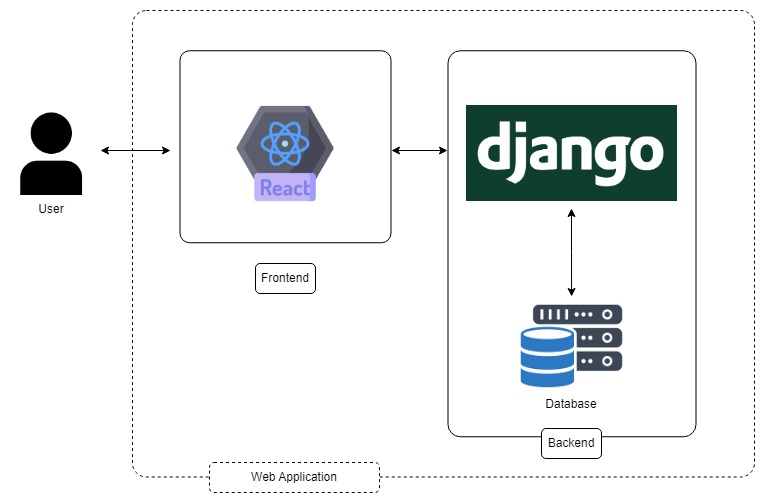
\includegraphics[width=\textwidth, keepaspectratio=true]{image/chap3/System Architecture.jpg}}
	\caption{แผนภาพที่แสดงสถาปัตยกรรมระบบ}\label{fig:SystemArchitecture}
\end{figure}

\hspace{1cm}
จากรูปภาพที่ \ref{fig:SystemArchitecture} ในเว็บแอปพลิเคชันจะแบ่งเป็นสองส่วนใหญ่ ๆ คือ Frontend และ Backend โดยผู้ใช้จะติดต่อกับเว็บแอปพลิเคชันผ่านทาง
Frontend ที่พัฒนาโดยใช้ React.js และ Frontend จะติดต่อกับ Backend ที่พัฒนาโดยใช้ Django และ Django
จะรับหน้าที่ในการติดต่อกับฐานข้อมูล

\pagebreak
\section{Sequence Diagram}

\subsubsection{ลงทะเบียนผู้ใช้งาน}
\hspace{1cm}
เมื่อผู้ใช้กดปุ่ม Log In แล้ว UI จะร้องขอข้อมูลการลงทะเบียน เมื่อผู้ใช้ส่งข้อมูล UI จะส่งข้อมูลไปที่ Application
เพื่อเพิ่มผู้ใช้ใหม่ และ Application ก็จะเพิ่มข้อมูลลงไปในฐานข้อมูล จากนั้นจึงส่งข้อมูลว่าลงทะเบียนสำเร็จ
และ UI จะแสดงผลว่าลงทะเบียนสำเร็จ ซึ่งสามารถแสดงผลลัพธ์การทำงานได้ดังรูปที่ \ref{fig:S_Register}
\begin{figure}[!h]\centering
	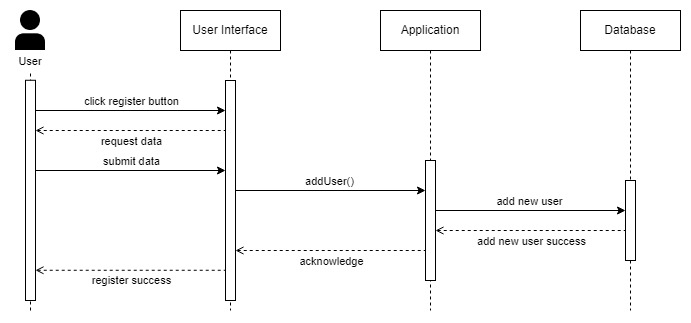
\includegraphics[width=\textwidth, keepaspectratio=true]{image/chap3/sequence/Register.jpg}
	\caption{แผนผังการทำงานแบบลำดับปฏิสัมพันธ์ของการลงทะเบียนผู้ใช้งาน}\label{fig:S_Register}
\end{figure}

\subsubsection{เข้าสู่ระบบ}
\hspace{1cm}
เมื่อผู้ใช้กดปุ่ม Log In แล้ว UI จะร้องขอข้อมูลการเข้าสู่ระบบ เมื่อผู้ใช้ส่งข้อมูล UI จะส่งข้อมูลไปที่ Application
เพื่อเข้าสู่ระบบ และ Application ก็จะเช็คความถูกต้องกับฐานข้อมูล จากนั้นจึงส่งข้อมูลว่าเข้าสู่ระบบสำเร็จ
และ UI จะแสดงผลว่าเข้าสู่ระบบสำเร็จ ซึ่งสามารถแสดงผลลัพธ์การทำงานได้ดังรูปที่ \ref{fig:S_LogIn}
\begin{figure}[!h]\centering
	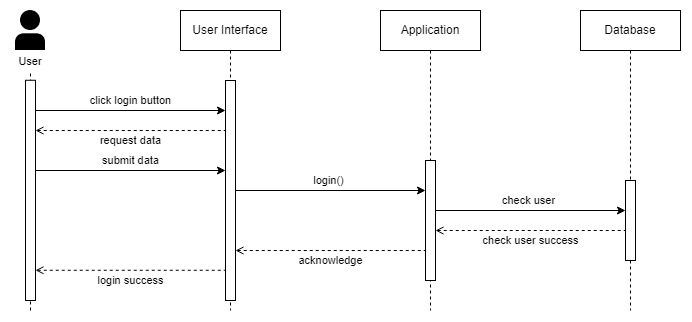
\includegraphics[width=\textwidth, keepaspectratio=true]{image/chap3/sequence/Login.jpg}
	\caption{แผนผังการทำงานแบบลำดับปฏิสัมพันธ์ของการเข้าสู่ระบบ}\label{fig:S_LogIn}
\end{figure}

\pagebreak
\subsubsection{ดูสถิติการใช้งานเว็บแอปพลิเคชัน}
\hspace{1cm}
เมื่อผู้ใช้กดปุ่มดูสถิติการใช้งานเว็บแอปพลิเคชัน UI จะร้องขอข้อมูลสถิติจากฐานข้อมูลผ่าน Application
และฐานข้อมูลจะส่งข้อมูลกลับมาให้ UI เพื่อแสดงผลสถิติการใช้งาน ซึ่งสามารถแสดงผลลัพธ์การทำงานได้ดังรูปที่ \ref{fig:S_Statistic}
\begin{figure}[!h]\centering
	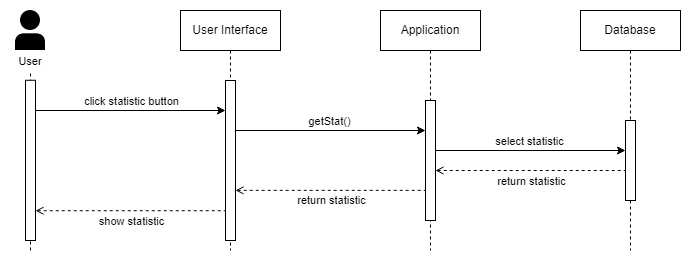
\includegraphics[width=\textwidth, keepaspectratio=true]{image/chap3/sequence/Statistic.jpg}
	\caption{แผนผังการทำงานแบบลำดับปฏิสัมพันธ์ของการดูสถิติการใช้งานเว็บแอปพลิเคชัน}\label{fig:S_Statistic}
\end{figure}

\subsubsection{ดูคำศัพท์ที่เคยเรียน}
\hspace{1cm}
เมื่อผู้ใช้กดปุ่มดูคำศัพท์ที่เคยเรียน UI จะร้องขอข้อมูลคำศัพท์ที่เคยเรียนจากฐานข้อมูลผ่าน Application
และฐานข้อมูลจะส่งข้อมูลกลับมาให้ UI เพื่อแสดงผลคำศัพท์ที่เคยเรียน ซึ่งสามารถแสดงผลลัพธ์การทำงานได้ดังรูปที่ \ref{fig:S_WordsLearned}
\begin{figure}[!h]\centering
	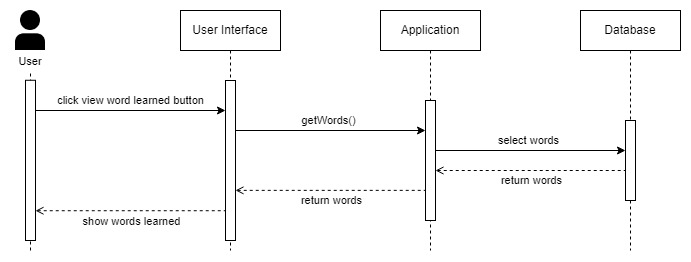
\includegraphics[width=\textwidth, keepaspectratio=true]{image/chap3/sequence/Words Learned.jpg}
	\caption{แผนผังการทำงานแบบลำดับปฏิสัมพันธ์ของการดูสถิติการใช้งานเว็บแอปพลิเคชัน}\label{fig:S_WordsLearned}
\end{figure}

\pagebreak
\subsubsection{ดูกระดานผู้นำ}
\hspace{1cm}
เมื่อผู้ใช้กดปุ่มดูกระดานผู้นำ UI จะร้องขอข้อมูลคะแนนของผู้ใช้จากฐานข้อมูลผ่าน Application
และฐานข้อมูลจะส่งข้อมูลกลับมาให้ UI เพื่อแสดงผลกระดานผู้นำ ซึ่งสามารถแสดงผลลัพธ์การทำงานได้ดังรูปที่ \ref{fig:S_Leaderboard}
\begin{figure}[!h]\centering
	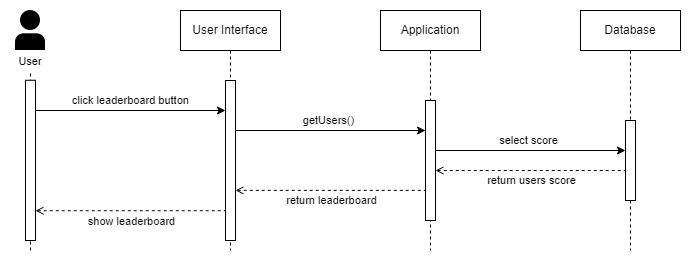
\includegraphics[width=\textwidth, keepaspectratio=true]{image/chap3/sequence/Leaderboard.jpg}
	\caption{แผนผังการทำงานแบบลำดับปฏิสัมพันธ์ของการดูกระดานผู้นำ}\label{fig:S_Leaderboard}
\end{figure}


\subsubsection{สุ่มคำศัพท์ใหม่เพื่อการเรียนรู้}
\hspace{1cm}
เมื่อผู้ใช้กดปุ่มสุ่มคำศัพท์ UI จะสุ่มคำศัพท์และร้องข้อมูลคำศัพท์จากฐานข้อมูลผ่าน Application
และฐานข้อมูลจะส่งข้อมูลกลับมาให้ UI เพื่อแสดงผลคำศัพท์ที่สุ่มมา ซึ่งสามารถแสดงผลลัพธ์การทำงานได้ดังรูปที่ \ref{fig:S_RandomWord}
\begin{figure}[!h]\centering
	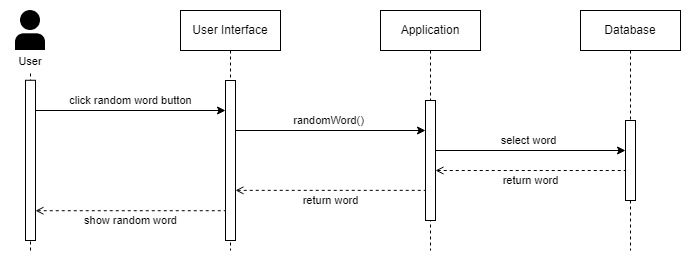
\includegraphics[width=\textwidth, keepaspectratio=true]{image/chap3/sequence/Random word.jpg}
	\caption{แผนผังการทำงานแบบลำดับปฏิสัมพันธ์ของการสุ่มคำศัพท์ใหม่เพื่อการเรียนรู้}\label{fig:S_RandomWord}
\end{figure}

\pagebreak
\subsubsection{ค้นหาคำศัพท์จากฐานข้อมูล}
\hspace{1cm}
เมื่อผู้ใช้กดปุ่มค้นหาคำศัพท์ UI จะร้องข้อมูลคำศัพท์ที่ต้องกับคำค้นหาจากฐานข้อมูลผ่าน Application
และฐานข้อมูลจะส่งข้อมูลกลับมาให้ UI เพื่อแสดงผลคำศัพท์ที่ค้นหา ซึ่งสามารถแสดงผลลัพธ์การทำงานได้ดังรูปที่ \ref{fig:S_SearchWord}
\begin{figure}[!h]\centering
	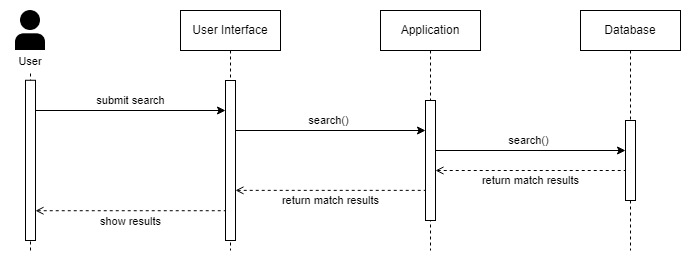
\includegraphics[width=\textwidth, keepaspectratio=true]{image/chap3/sequence/Search.jpg}
	\caption{แผนผังการทำงานแบบลำดับปฏิสัมพันธ์ของการค้นหาคำศัพท์จากฐานข้อมูล}\label{fig:S_SearchWord}
\end{figure}


\subsubsection{แสดงผลรายละเอียดคำศัพท์}
\hspace{1cm}
เมื่อผู้ใช้กดปุ่มแสดงผลรายละเอียดคำศัพท์ UI จะร้องข้อมูลคำศัพท์ดังกล่าวจากฐานข้อมูลผ่าน Application
และฐานข้อมูลจะส่งข้อมูลกลับมาให้ UI เพื่อแสดงผลรายละเอียดคำศัพท์ที่ผู้ใช้กด ซึ่งสามารถแสดงผลลัพธ์การทำงานได้ดังรูปที่ \ref{fig:S_WordDetail}
\begin{figure}[!h]\centering
	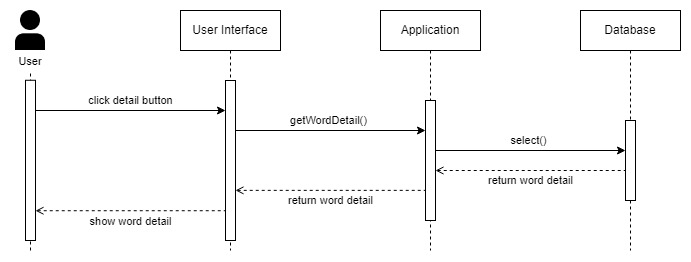
\includegraphics[width=\textwidth, keepaspectratio=true]{image/chap3/sequence/View-Search.jpg}
	\caption{แผนผังการทำงานแบบลำดับปฏิสัมพันธ์ของการแสดงผลรายละเอียดคำศัพท์}\label{fig:S_WordDetail}
\end{figure}


% \subsubsection{เลือกคำศัพท์เพื่อใช้งานบัตรคำ}
% \hspace{1cm}
% เมื่อผู้ใช้กดปุ่มเลือกคำศัพท์เพื่อใช้งานบัตรคำ UI จะสุ่มคำศัพท์และร้องข้อมูลคำศัพท์จากฐานข้อมูลผ่าน Application
% และฐานข้อมูลจะส่งข้อมูลกลับมาให้ UI เพื่อแสดงผลคำศัพท์ดังกล่าว และเมื่อผู้ใช้ทำการเลือกคำศัพท์นั้นเพื่อใช้งานบัตรคำ
% UI จะส่งข้อมูลดังกล่าวไปเก็บไว้ที่ Application จากนั้นจะทำการสุ่มคำศัพท์ใหม่จนครบ 10 คำ ซึ่งสามารถแสดงผลลัพธ์การทำงานได้ดังรูปที่ \ref{fig:S_SelectFlashcard}
% \begin{figure}[!h]\centering
% 	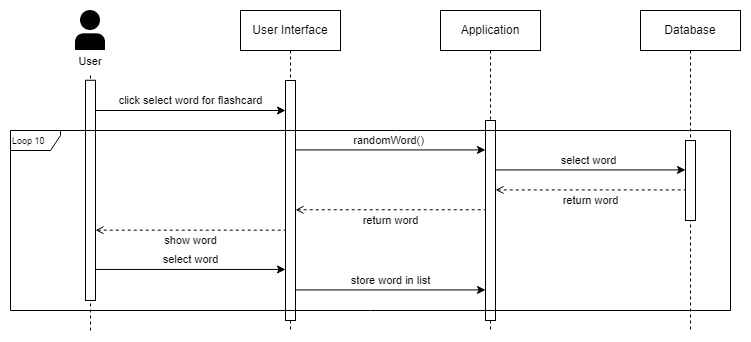
\includegraphics[width=\textwidth, keepaspectratio=true]{image/chap3/sequence/Flash-Select.jpg}
% 	\caption{แผนผังการทำงานแบบลำดับปฏิสัมพันธ์ของการเลือกคำศัพท์เพื่อใช้งานบัตรคำ}\label{fig:S_SelectFlashcard}
% \end{figure}

\pagebreak
\subsubsection{สุ่มคำศัพท์เพื่อใช้งานบัตรคำ}
\hspace{1cm}
เมื่อผู้ใช้กดปุ่มเริ่มใช้งานบัตรคำ UI จะสุ่มคำศัพท์และร้องข้อมูลคำศัพท์จากฐานข้อมูลผ่าน Application
และฐานข้อมูลจะส่งข้อมูลกลับมาที่ Application และทำการเก็บข้อมูลไว้ จากนั้นจะทำการสุ่มคำศัพท์ใหม่จนครบ 5 คำ
ซึ่งสามารถแสดงผลลัพธ์การทำงานได้ดังรูปที่ \ref{fig:S_RandomFlashcard}
\begin{figure}[!h]\centering
	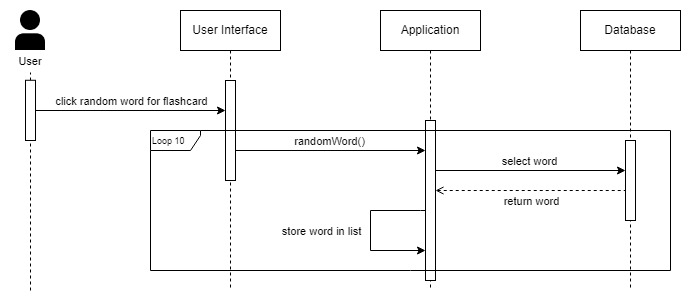
\includegraphics[width=\textwidth, keepaspectratio=true]{image/chap3/sequence/Flash-Random.jpg}
	\caption{แผนผังการทำงานแบบลำดับปฏิสัมพันธ์ของการสุ่มคำศัพท์เพื่อใช้งานบัตรคำ}\label{fig:S_RandomFlashcard}
\end{figure}

\pagebreak
\subsubsection{ดูบัตรคำ}
\hspace{1cm}
UI จะร้องขอข้อมูลคำศัพท์ที่เก็บไว้ใน Application มาทำการแสดงผลด้านหน้าของบัตรคำ และเมื่อผู้ใช้กดที่บัตรคำ UI จะทำการแสดงผลด้านหลังของบัตรคำ
และเมื่อผู้ใช้กดจำบัตรคำ UI จะทำการลบคำดังกล่าวและร้องขอข้อมูลคำศัพท์ถัดไปจาก Application และ Application จะทำการส่งข้อมูลคำศัพท์เข้าไปเก็บเป็นคำศัพท์ที่เรียนแล้ว
ในฐานข้อมูล แล้วจึงส่งข้อมูลคำศัพท์ถัดไปมาให้ UI เพื่อแสดงผล จากนั้นจะทำการแสดงผลคำศัพท์ถัดไปจนไม่เหลือคำศัพท์อยู่ และ UI จะทำการ
ส่งคำศัพท์ไปเก็บเป็นคำศัพท์ที่เคยเรียนแล้วใน Database ผ่าน Application ซึ่งสามารถแสดงผลลัพธ์การทำงานได้ดังรูปที่ \ref{fig:S_Flashcard}
\begin{figure}[!h]\centering
	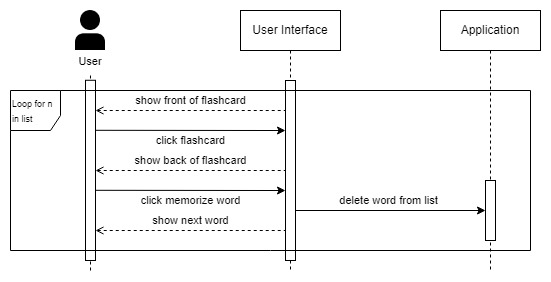
\includegraphics[width=\textwidth, keepaspectratio=true]{image/chap3/sequence/Flashcard.jpg}
	\caption{แผนผังการทำงานแบบลำดับปฏิสัมพันธ์ของการดูบัตรคำ}\label{fig:S_Flashcard}
\end{figure}

\pagebreak
\subsubsection{ทำแบบทดสอบ}
\hspace{1cm}
เมื่อผู้ใช้กดปุ่มเริ่มทำแบบทดสอบ ระบบจะทำการสุ่มคำศัพท์จำนวน 10 คำมาเก็บไว้ใน Application จากนั้นจะส่งรายการคำศัพท์ไปให้ UI เพื่อทำการแสดงแบบทดสอบ
เมื่อ UI แสดงแบบทดสอบแล้ว ผู้ใช้จะตอบคำถาม จากนั้น UI จะแสดงผลคำตอบที่ถูกต้อง แล้ววนซ้ำการแสดงผลแบบทดสอบจนครบ 10 รอบ จากนั้นจึงแสดงผลลัพท์ของการทำแบบทดสอบ
และ UI จะทำการส่งสถิติและคะแนนไปเก็บใน Database ผ่าน Application ซึ่งสามารถแสดงผลลัพธ์การทำงานได้ดังรูปที่ \ref{fig:S_Quiz}
\begin{figure}[!h]\centering
	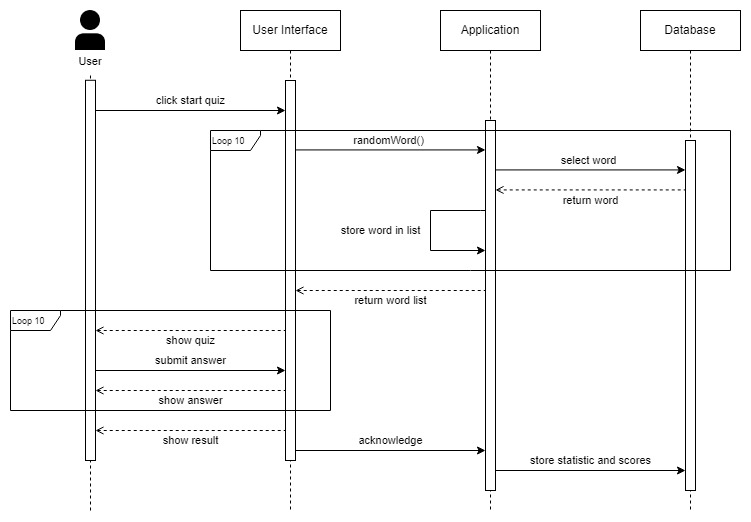
\includegraphics[width=\textwidth, keepaspectratio=true]{image/chap3/sequence/Quiz.jpg}
	\caption{แผนผังการทำงานแบบลำดับปฏิสัมพันธ์ของการทำแบบทดสอบ}\label{fig:S_Quiz}
\end{figure}

\pagebreak
\subsubsection{เล่นเกมเรียงพยัญชนะเป็นคำศัพท์}
\hspace{1cm}
เมื่อผู้ใช้กดปุ่มเริ่มเล่นเกมระบบจะทำการสุ่มคำศัพท์จากฐานข้อมูลผ่าน Application เพื่อทำการแสดงผลคำศัพท์ที่ใช้เล่นเกม เมื่อได้คำศัพท์แล้ว
UI จะแสดงผลคำศัพท์ที่ใช้เล่นเกม ผู้ใช้จะใส่คำตอบ จากนั้น UI จะแสดงผลคำตอบที่ถูกต้อง จากนั้นจึงแสดงผลลัพท์ของการเล่นเกม
และ UI จะทำการส่งสถิติและคะแนนไปเก็บใน Database ผ่าน Application ซึ่งสามารถแสดงผลลัพธ์การทำงานได้ดังรูปที่ \ref{fig:S_Game}
\begin{figure}[!h]\centering
	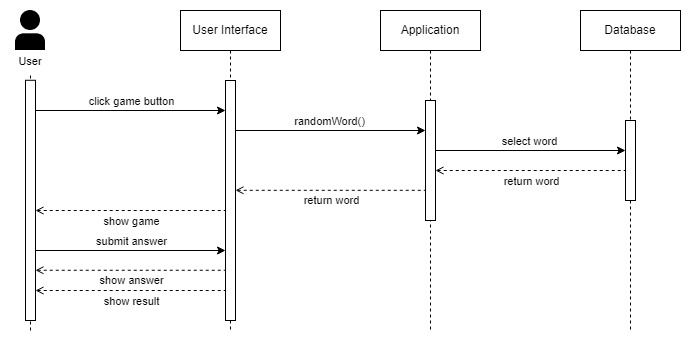
\includegraphics[width=\textwidth, keepaspectratio=true]{image/chap3/sequence/Game.jpg}
	\caption{แผนผังการทำงานแบบลำดับปฏิสัมพันธ์ของการเล่นเกมเรียงพยัญชนะเป็นคำศัพท์}\label{fig:S_Game}
\end{figure}

\pagebreak
\section{User Interface Design} \label{ssec:UI}
\subsection{หน้าหลัก}
\begin{figure}[!h]\centering
	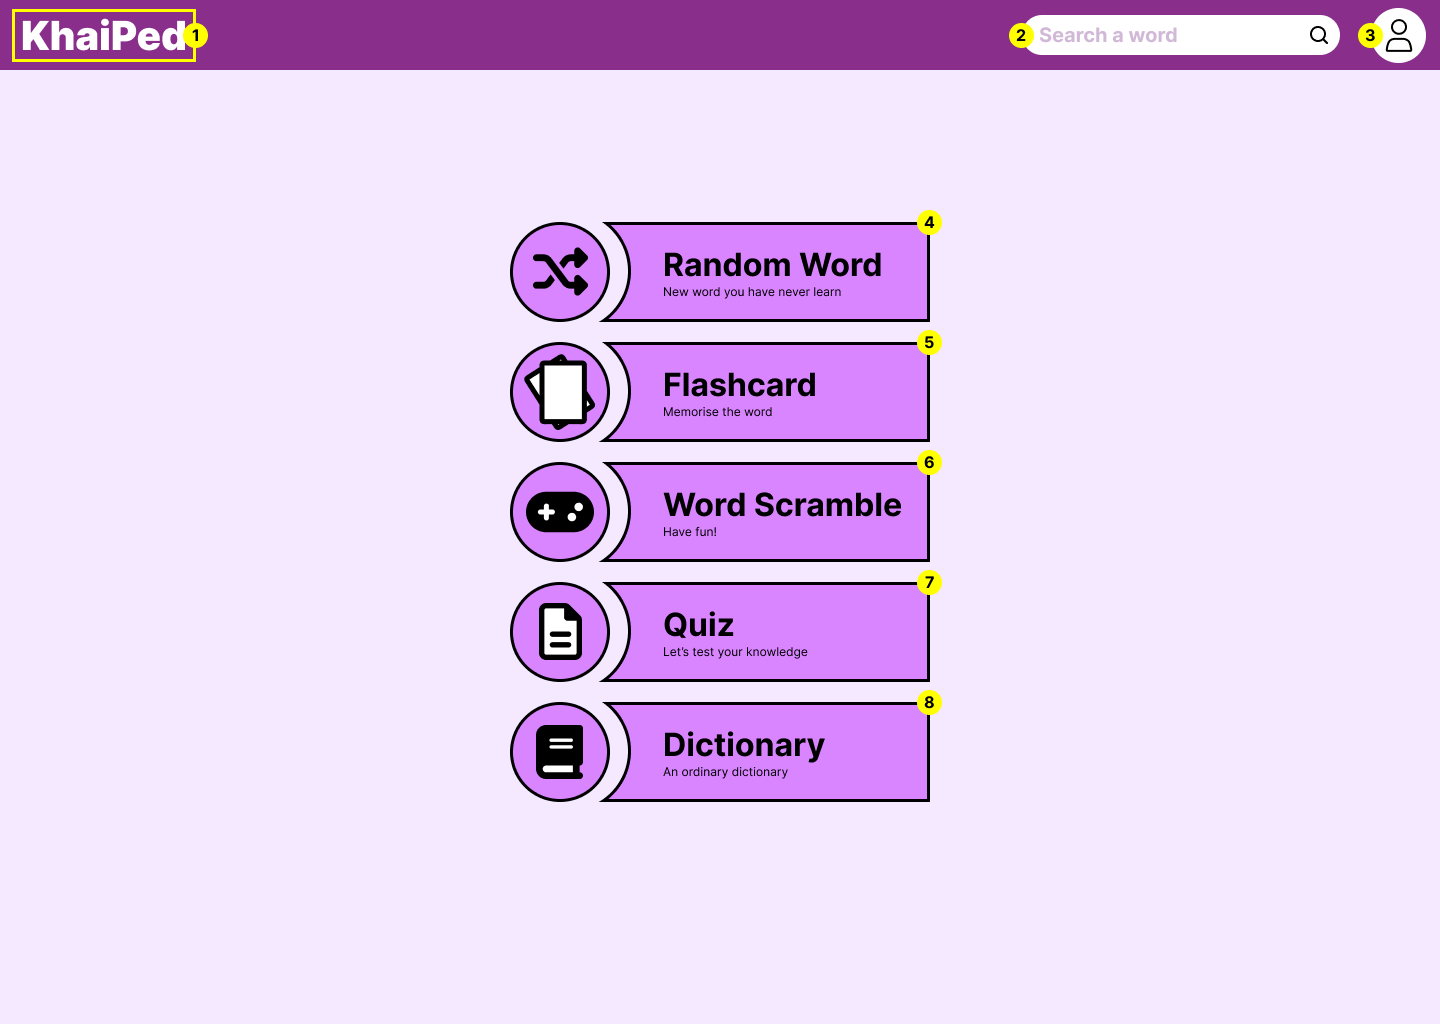
\includegraphics[width=0.8\textwidth, keepaspectratio=true]{image/chap3/ui/Home page.png}
	\caption{หน้าหลัก}\label{fig:UI_Home}
\end{figure}
\hspace{1cm}
หน้าหลักสำหรับผู้ใช้งาน ซึ่งแสดงให้เห็นดังรูปภาพที่ \ref{fig:UI_Home} ประกอบด้วยปุ่มโลโก้ (1) ที่สามารถกดเพื่อกลับมาหน้าหลักได้ ช่องค้นหาคำศัพท์ (2) เพื่อค้นหาคำศัพท์ในฐานข้อมูล
ปุ่มผู้ใช้ (3) สำหรับลงทะเบียนหรือเข้าสู่ระบบ และปุ่มสำหรับการใช้งานฟีเจอร์ต่าง ๆ ของระบบ ประกอบด้วย
ปุ่มสุ่มคำศัพท์ (4) เพื่อสุ่มคำศัพท์ภาษาอังกฤษใหม่ ๆ ที่ยังไม่เคยเรียน ปุ่มบัตรคำ (5) เพื่อใช้งานบัตรคำ ปุ่มเล่นเกม (6) เพื่อเล่นเกมเรียงพยัญชนะเป็นคำศัพท์
ปุ่มทำแบบทดสอบ (7) เพื่อเข้าทำแบบทดสอบ ปุ่มพจนานุกรม (8) เพื่อใช้งานพจนานุกรม และปุ่มช่วยเหลือ (9) เพื่อดูวิธีการใช้งานเว็บแอปพลิชันได้

\pagebreak
\begin{figure}[!h]\centering
	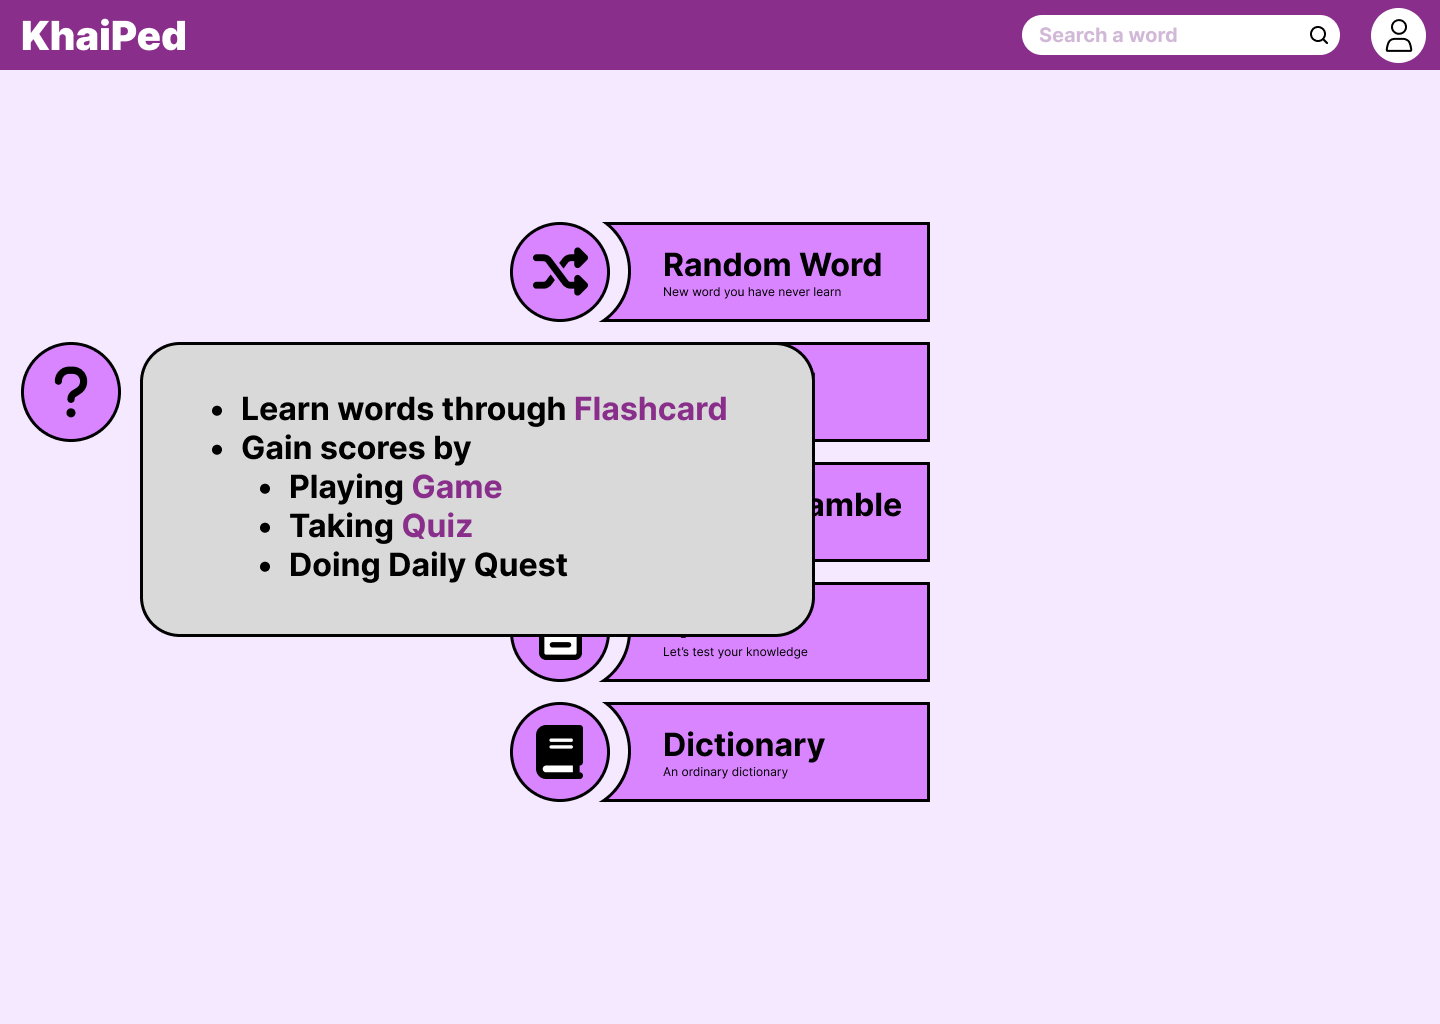
\includegraphics[width=0.8\textwidth, keepaspectratio=true]{image/chap3/ui/Home page - Help.png}
	\caption{ปุ่มช่วยเหลือหน้าหลัก}\label{fig:UI_HomeHelp}
\end{figure}
\hspace{1cm}
จากรูปภาพที่ \ref{fig:UI_Home} เมื่อกดปุ่มช่วยเหลือในหน้าหลัก จะแสดงผลกล่องข้อความที่แสดงวิธีการใช้งานเว็บแอปพลิเคชัน ซึ่งแสดงให้เห็นดังรูปภาพที่ \ref{fig:UI_HomeHelp}

\pagebreak
\subsection{การลงทะเบียนผู้ใช้และเข้าสู่ระบบ}
\begin{figure}[!h]\centering
	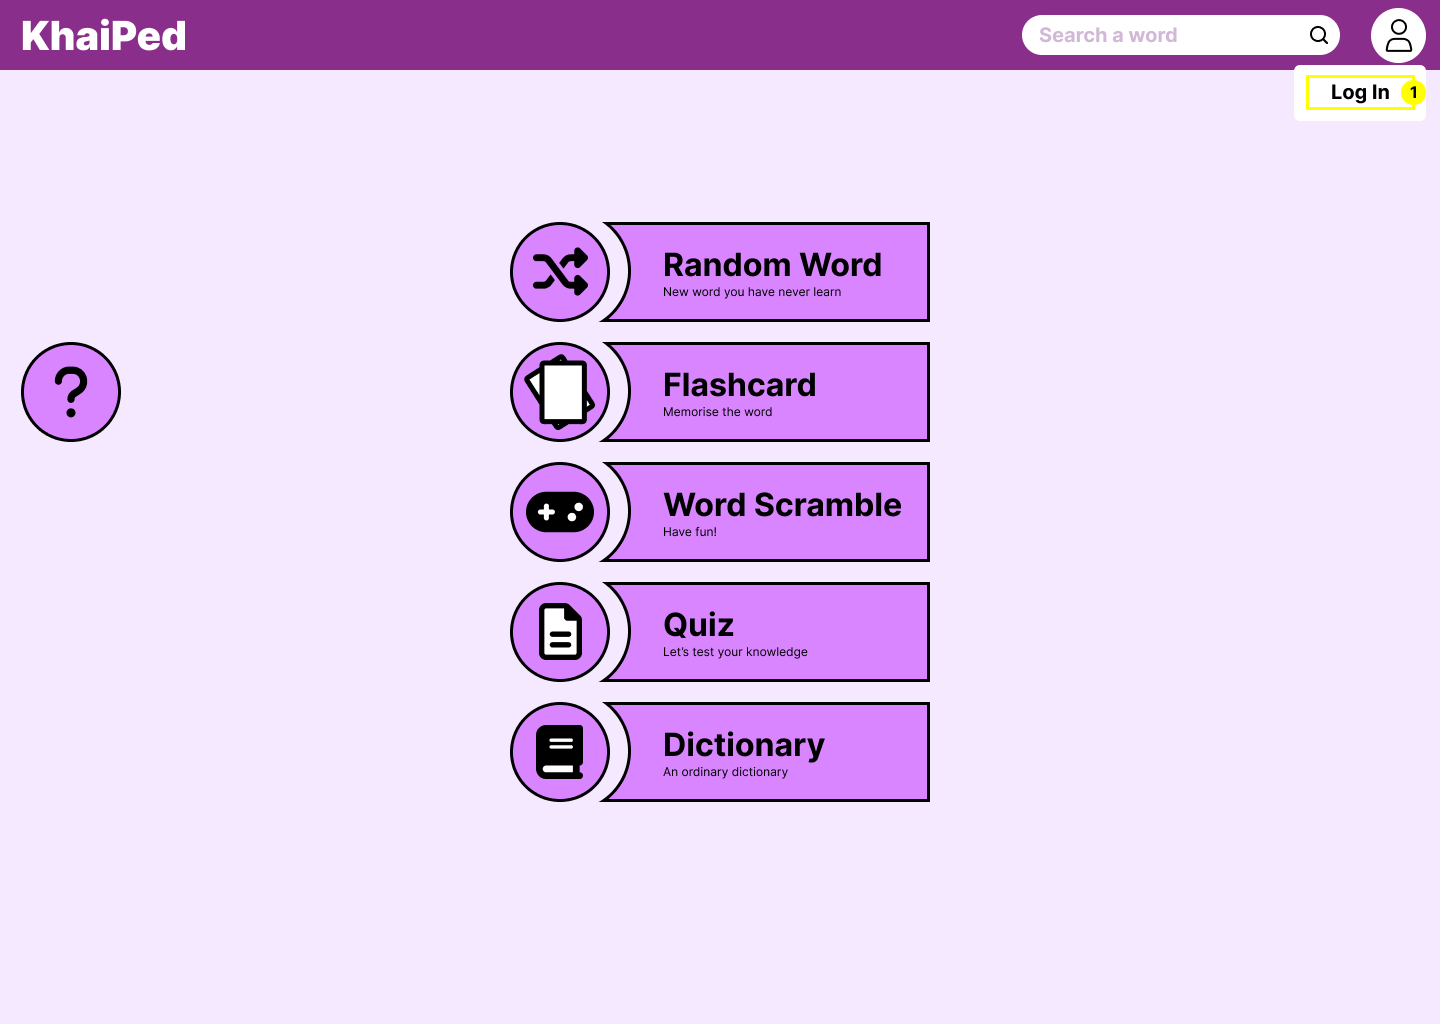
\includegraphics[width=0.8\textwidth, keepaspectratio=true]{image/chap3/ui/login/Home page - Guest User Button.png}
	\caption{ปุ่มผู้ใช้หากไม่ได้เข้าสู่ระบบ}\label{fig:UI_GuestButton}
\end{figure}
\hspace{1cm}
เมื่อผู้ใช้งานกดปุ่มผู้ใช้โดยที่ยังไม่ได้เข้าสู่ระบบ จะระบบจะแสดงปุ่มเข้าสู่ระบบ (1) สำหรับผู้ใช้งานที่มีบัญชีอยู่แล้วเพื่อเข้าสู่ระบบ
ซึ่งแสดงให้เห็นดังรูปภาพที่ \ref{fig:UI_GuestButton}


\begin{figure}[!h]\centering
	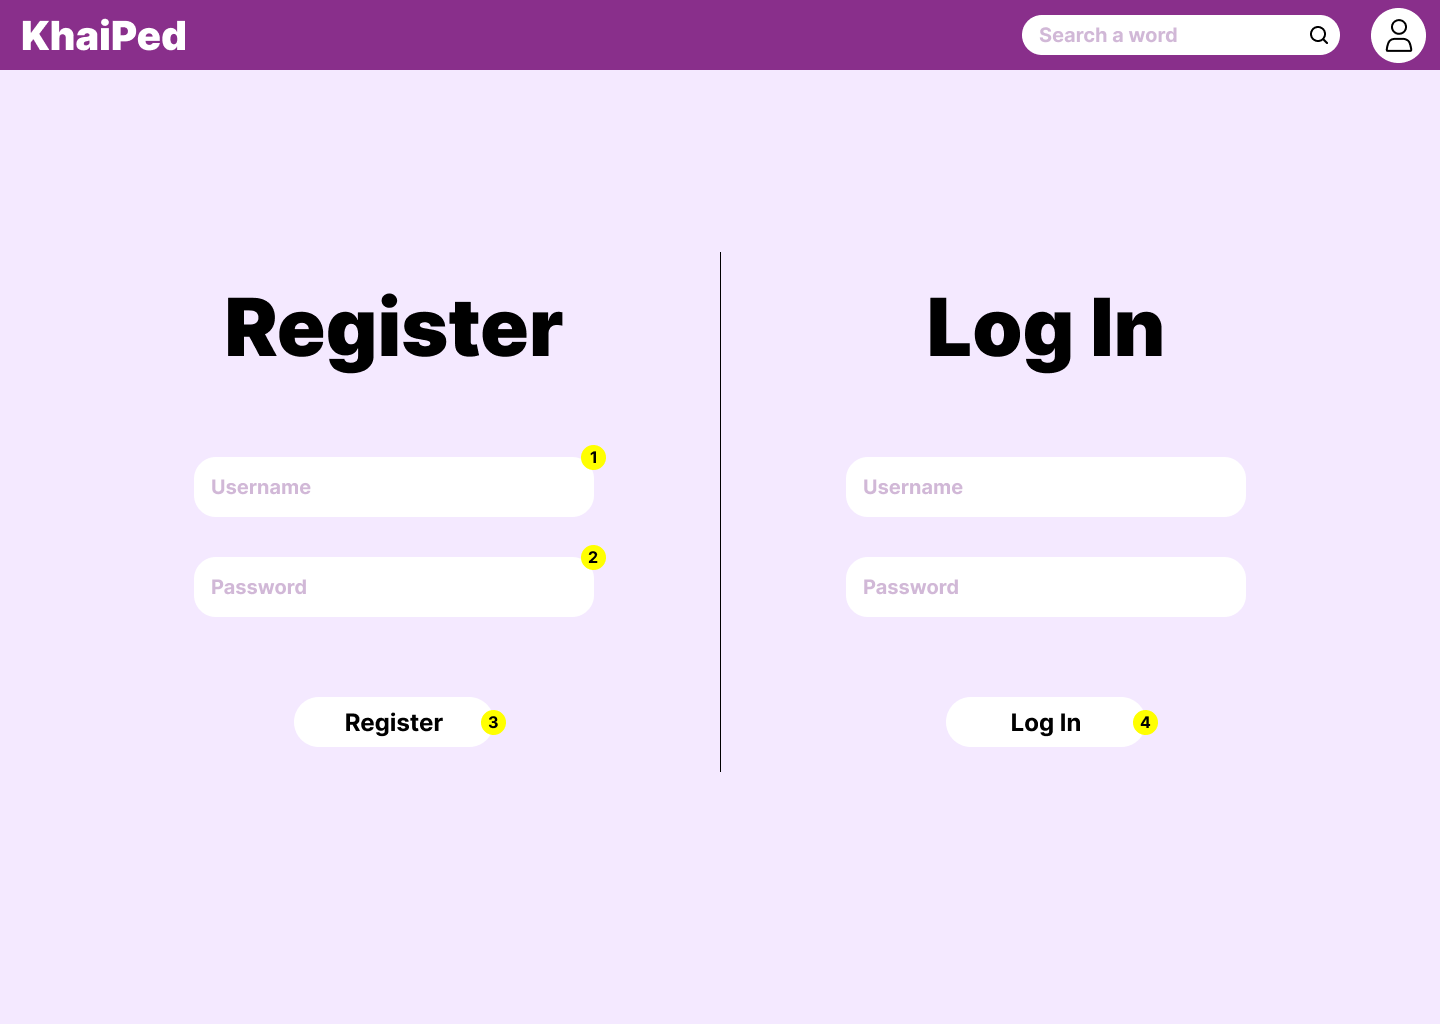
\includegraphics[width=0.8\textwidth, keepaspectratio=true]{image/chap3/ui/login/Home page - Register.png}
	\caption{หน้าลงทะเบียนและเข้าสู่ระบบ}\label{fig:UI_LoginPage}
\end{figure}
\hspace{1cm}
จากรูปภาพที่ \ref{fig:UI_GuestButton} เมื่อผู้ใช้งานกดปุ่มเข้าสู่ระบบ ระบบจะแสดงผลหน้าลงทะเบียนและเข้าสู่ระบบ โดยจะประกอบไปด้วยส่วนสำหรับใส่ชื่อผู้ใช้งาน (1)
ส่วนสำหรับใส่รหัสผ่าน (2) ปุ่มลงทะเบียน (3) และ ปุ่มเข้าสู่ระบบ (4) ดังรูปภาพที่ \ref{fig:UI_LoginPage}

\pagebreak
\begin{figure}[!h]\centering
	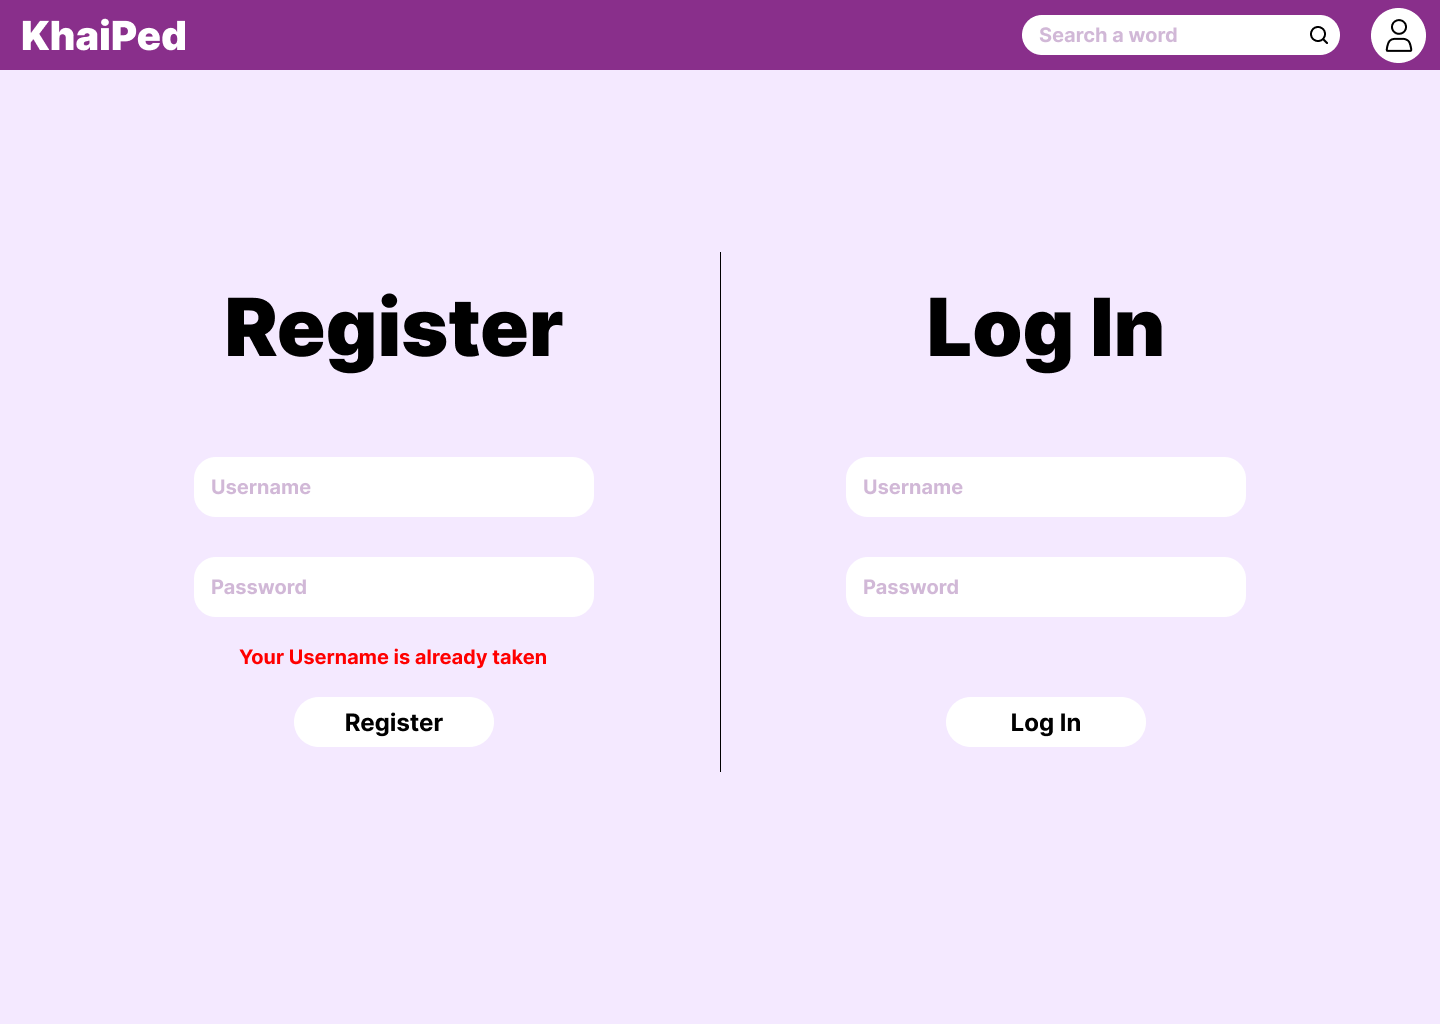
\includegraphics[width=0.8\textwidth, keepaspectratio=true]{image/chap3/ui/login/Home page - Register error.png}
	\caption{ข้อผิดพลาดในการลงทะเบียน}\label{fig:UI_RegisterError}
\end{figure}
\hspace{1cm}
หากผู้ใช้งานกรอกชื่อผู้ใช้งานที่ซ้ำกับในระบบ ระบบจะแจ้งเตือนว่าชื่อผู้ใช้งานได้ถูกใช้ไปแล้ว ซึ่งแสดงให้เห็นดังรูปภาพที่ \ref{fig:UI_RegisterError}

\begin{figure}[!h]\centering
	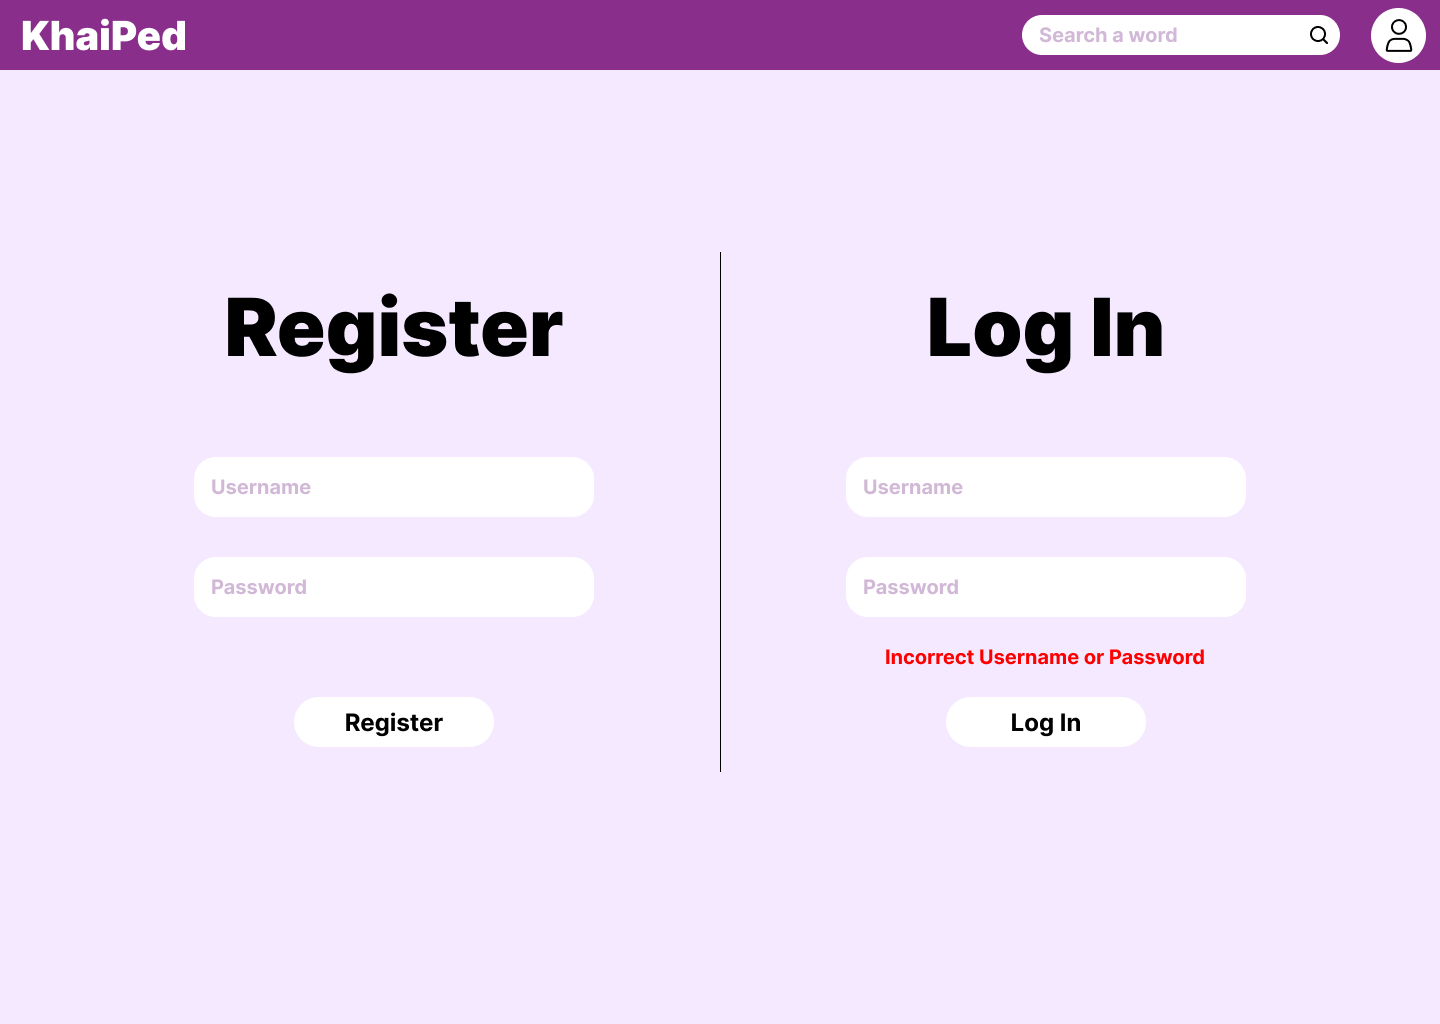
\includegraphics[width=0.8\textwidth, keepaspectratio=true]{image/chap3/ui/login/Home page - Log in error.png}
	\caption{ข้อผิดพลาดในการเข้าสู่ระบบ}\label{fig:UI_LogInError}
\end{figure}
\hspace{1cm}
หากผู้ใช้งานกรอกชื่อผู้ใช้งานหรือรหัสผ่านผิด ระบบจะแจ้งเตือนว่าชื่อผู้ใช้งานหรือรหัสผ่านผิด ซึ่งแสดงให้เห็นดังรูปภาพที่ \ref{fig:UI_LogInError}

\pagebreak
\begin{figure}[!h]\centering
	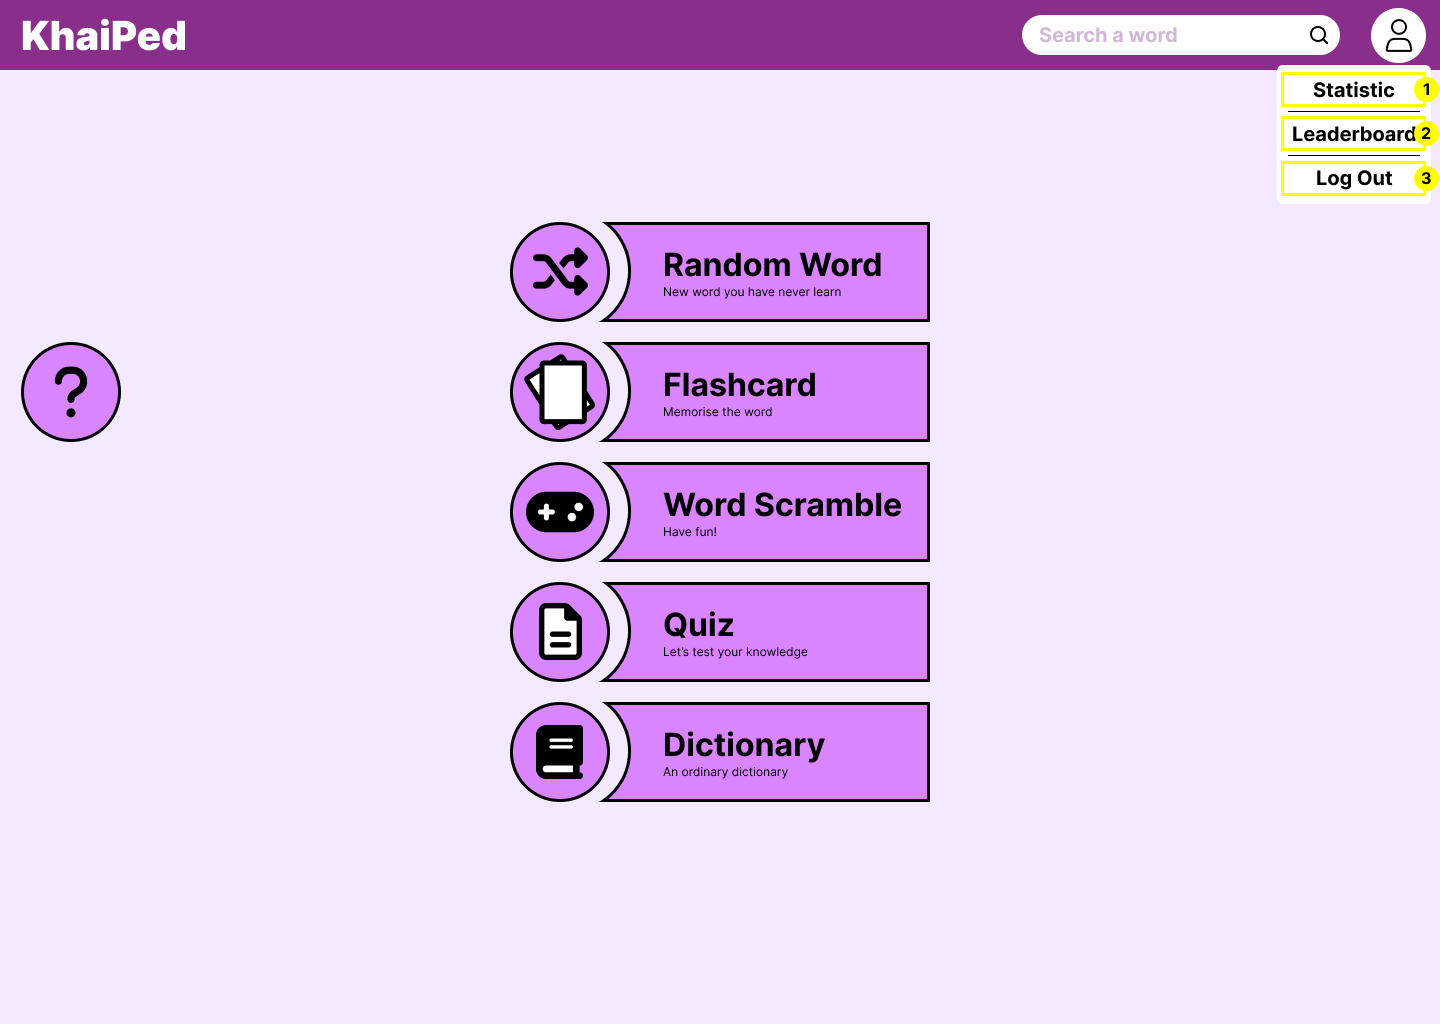
\includegraphics[width=0.8\textwidth, keepaspectratio=true]{image/chap3/ui/statistic/Home page - Logged In User Button.png}
	\caption{ปุ่มผู้ใช้หากเข้าสู่ระบบแล้ว}\label{fig:UI_UserButton}
\end{figure}
\hspace{1cm}
เมื่อผู้ใช้งานกดปุ่มผู้ใช้โดยที่เข้าสู่ระบบแล้ว จะระบบจะแสดงปุ่มสองปุ่มคือ ปุ่มสถิติ (1) เพื่อเข้าสู่หน้าแสดงผลสถิติการใช้เว็บแอปพลิเคชันของผู้ใช้
ปุ่มกระดานผู้นำ (2) เพื่อเข้าสู่หน้าแสดงผลกระดานผู้นำ และปุ่มลงชื่อออก (3)
ซึ่งแสดงให้เห็นดังรูปภาพที่ \ref{fig:UI_UserButton}

\pagebreak
\subsection{หน้าสถิติการใช้งานเว็บแอปพลิเคชัน}
\begin{figure}[!h]\centering
	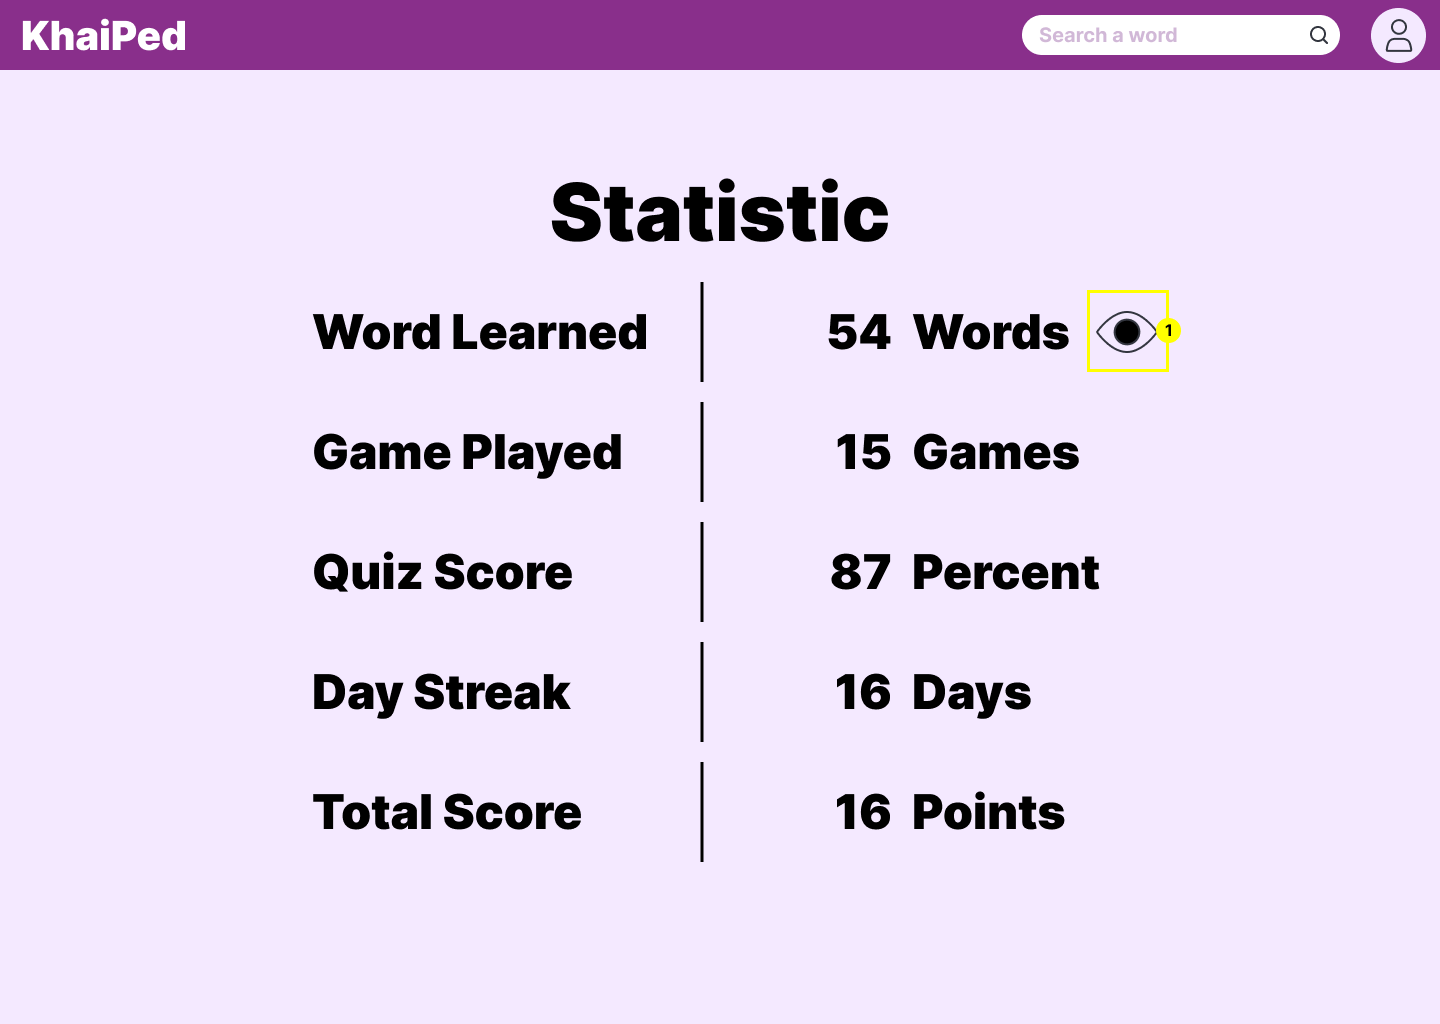
\includegraphics[width=0.8\textwidth, keepaspectratio=true]{image/chap3/ui/statistic/Statistic.png}
	\caption{หน้าสถิติการใช้งานเว็บแอปพลิเคชัน}\label{fig:UI_Statistic}
\end{figure}
\hspace{1cm}
จากรูปภาพที่ \ref{fig:UI_UserButton} เมื่อผู้ใช้งานกดปุ่มสถิติ ระบบจะแสดงผลหน้าสถิติ ซึ่งแสดงให้เห็นดังรูปภาพที่ \ref{fig:UI_Statistic}
โดยภายในหน้าประกอบไปด้วยจำนวนคำที่เคยเรียน จำนวนเกมที่ได้เล่นไป คะแนนของแบบทดสอบโดยคิดเป็นเปอร์เซ็นต์ และจำนวนวันที่เข้าใช้งานติดต่อกัน
และปุ่มดูคำศัพท์ที่เคยเรียน (1) เมื่อกดแล้วจะสามารถดูคำศัพท์ที่เคยเรียนไปแล้วได้

\begin{figure}[!h]\centering
	\includegraphics[width=0.8\textwidth, keepaspectratio=true]{image/chap3/ui/statistic/User’s Word Learned.png}
	\caption{หน้าคำศัพท์ที่ผู้ใช้ได้เคยเรียนรู้}\label{fig:UI_WordLearned}
\end{figure}
\hspace{1cm}
จากรูปภาพที่ \ref{fig:UI_Statistic} เมื่อผู้ใช้งานกดปุ่มดูคำศัพท์ที่เคยเรียน ระบบจะแสดงผลคำศัพท์ที่ผู้ใช้ได้เคยเรียนรู้มา ซึ่งแสดงให้เห็นดังรูปภาพที่ \ref{fig:UI_WordLearned}
โดยแต่ละคำศัพท์ จะมีปุ่มดูรายละเอียด (1) เพื่อดูรายละเอียดคำศัพท์นั้น ๆ ได้

\pagebreak
\begin{figure}[!h]\centering
	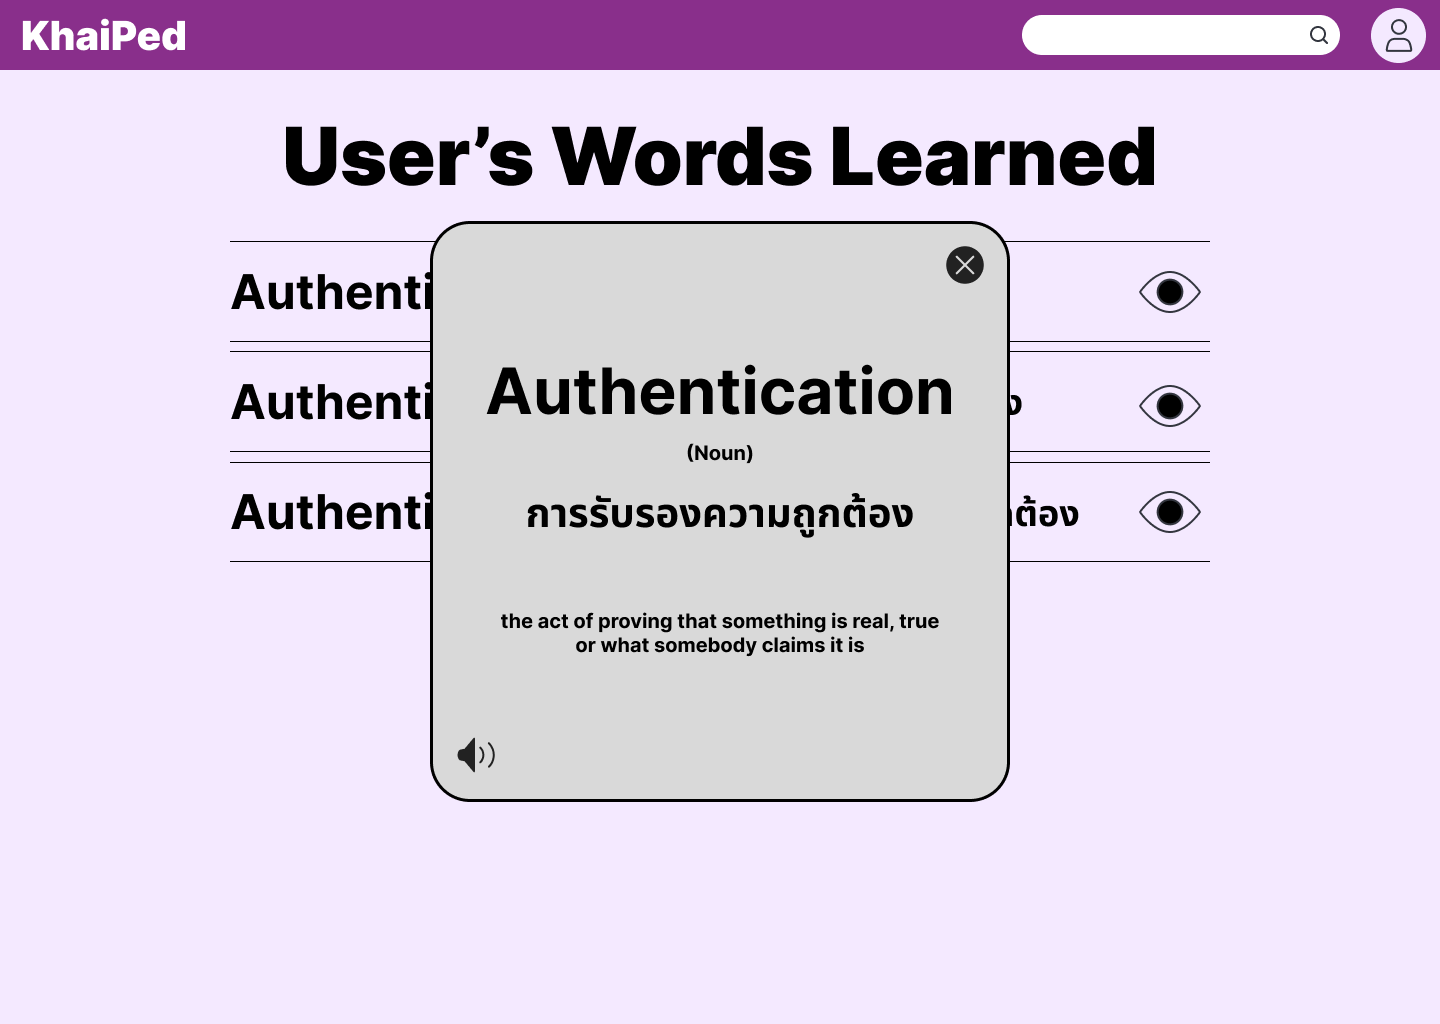
\includegraphics[width=0.8\textwidth, keepaspectratio=true]{image/chap3/ui/statistic/Word Learned detail.png}
	\caption{การแสดงผลรายละเอียดคำศัพท์}\label{fig:UI_WordLearnedDetail}
\end{figure}
\hspace{1cm}
จากรูปภาพที่ \ref{fig:UI_WordLearned} เมื่อผู้ใช้งานกดปุ่มดูรายละเอียด ระบบจะแสดงผลรายละเอียดของคำศัพท์ที่กด ซึ่งแสดงให้เห็นดังรูปภาพที่ \ref{fig:UI_WordLearnedDetail}

\pagebreak
\subsection{หน้ากระดานผู้นำ}
\begin{figure}[!h]\centering
	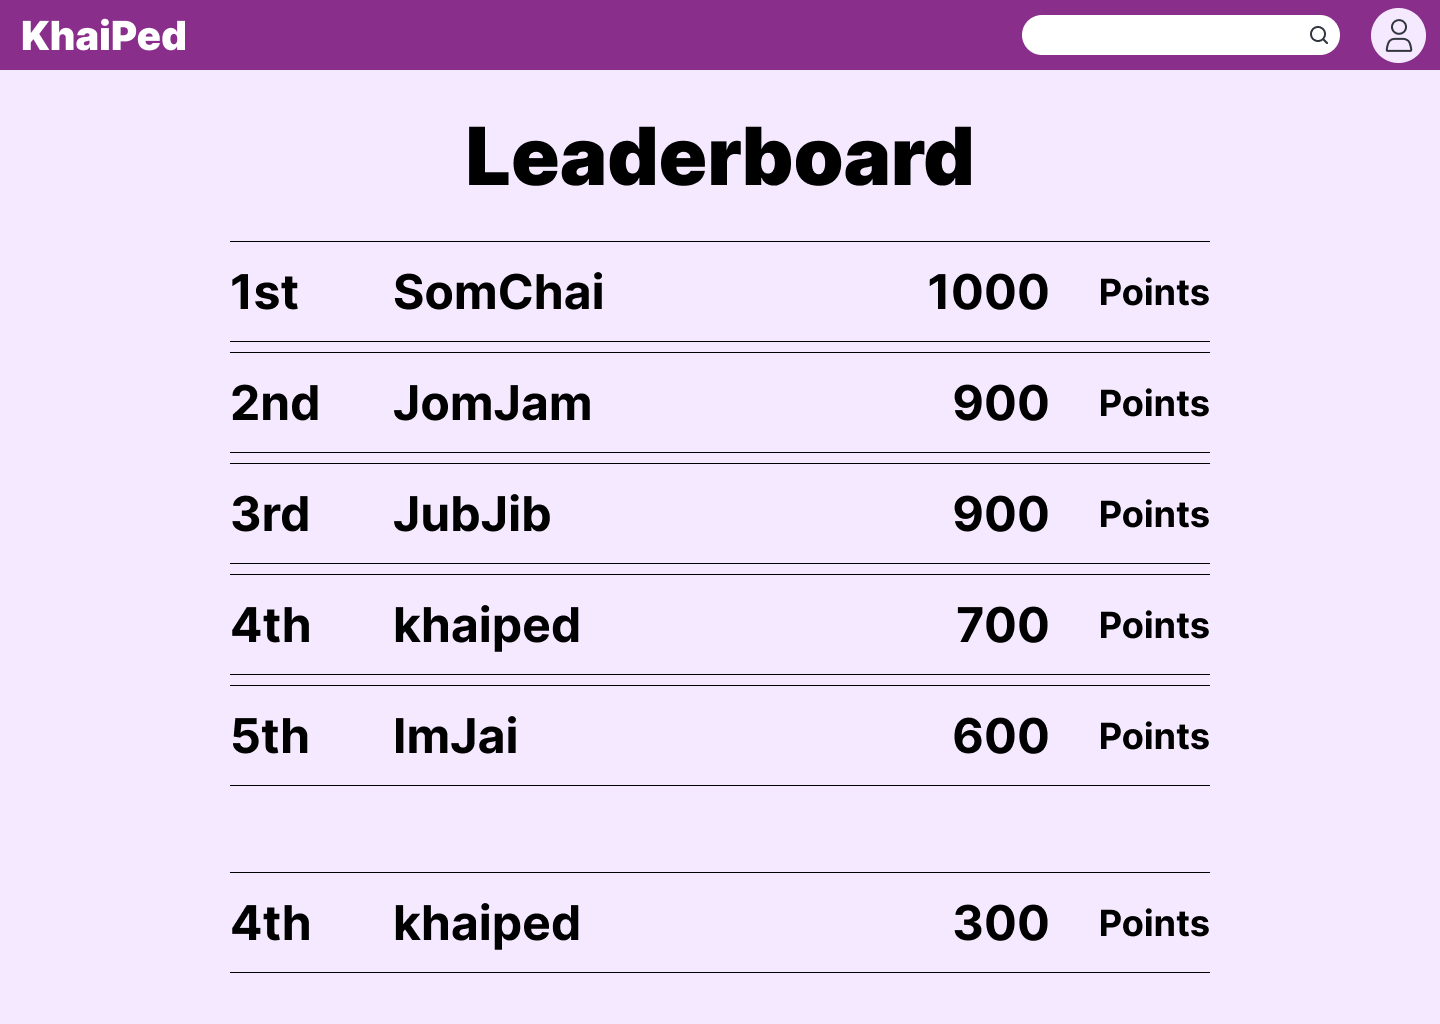
\includegraphics[width=0.8\textwidth, keepaspectratio=true]{image/chap3/ui/statistic/Leaderboard.png}
	\caption{หน้ากระดานผู้นำ}\label{fig:UI_Leaderboard}
\end{figure}
\hspace{1cm}
จากรูปภาพที่ \ref{fig:UI_UserButton} เมื่อผู้ใช้งานกดปุ่มปุ่มกระดานผู้นำ ระบบจะแสดงผลหน้ากระดานผู้นำ ซึ่งแสดงให้เห็นดังรูปภาพที่ \ref{fig:UI_Leaderboard}
ซึ่งจะประกอบไปด้วยผู้ใช้ 5 อันดับแรกที่มีคะแนนสูงสุด และจะแสดงลำดับของและคะแนนของผู้ใช้งานปัจจุบัน

\pagebreak
\subsection{การสุ่มคำศัพท์ใหม่เพื่อการเรียนรู้}
\begin{figure}[!h]\centering
	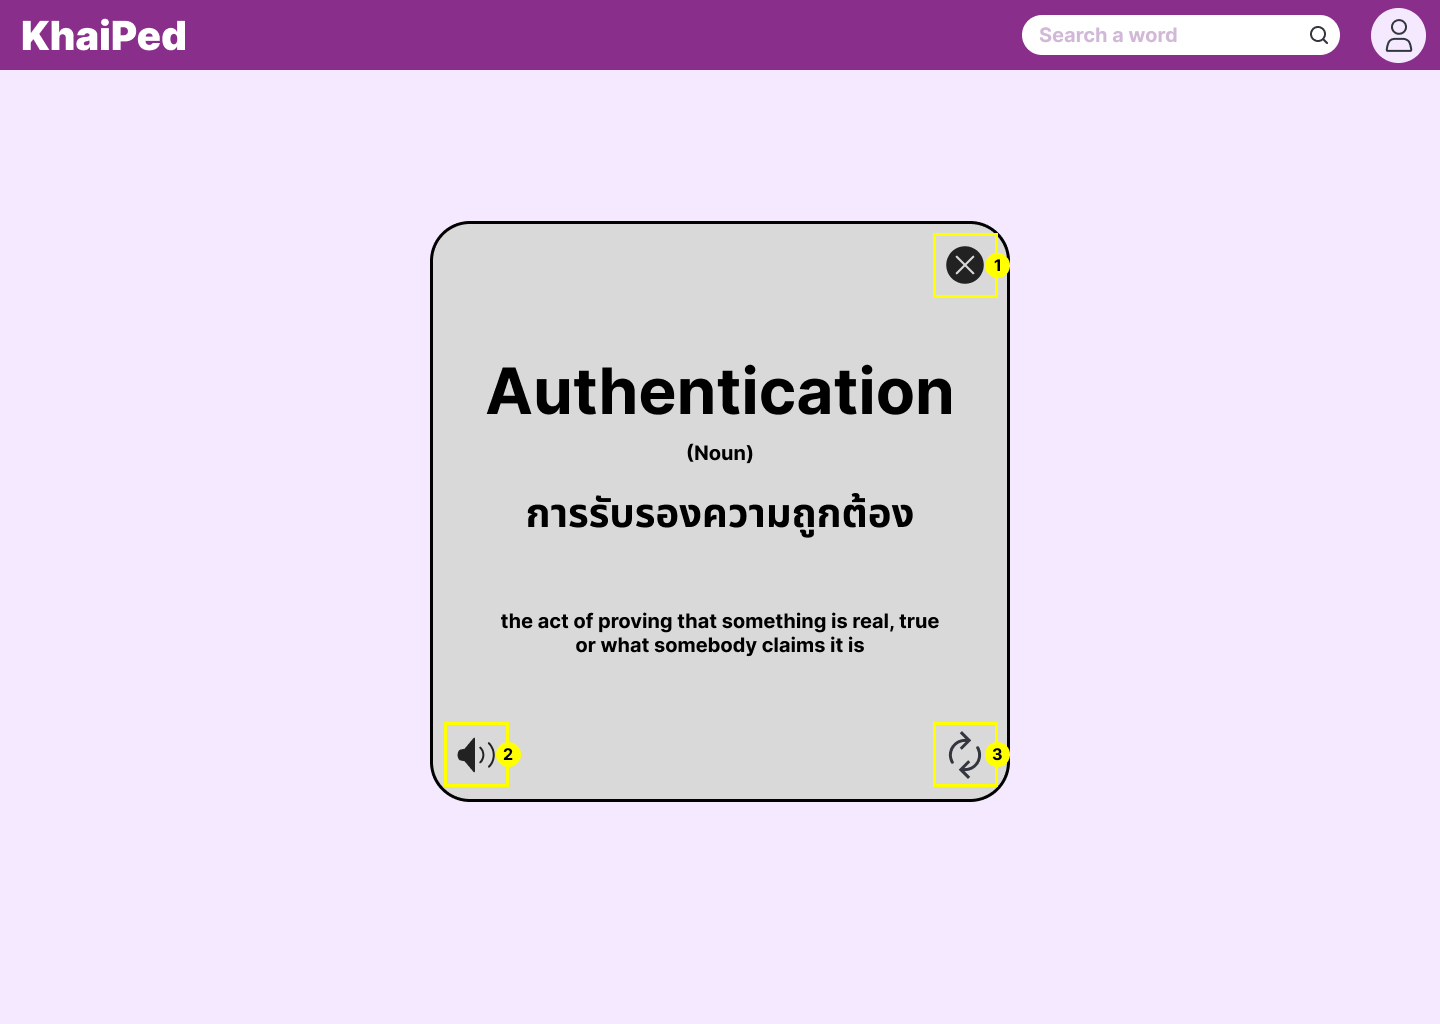
\includegraphics[width=0.8\textwidth, keepaspectratio=true]{image/chap3/ui/Random Word.png}
	\caption{การสุ่มคำศัพท์ใหม่เพื่อการเรียนรู้}\label{fig:UI_RandomWord}
\end{figure}
\hspace{1cm}
จากรูปภาพที่ \ref{fig:UI_Home} เมื่อผู้ใช้กดปุ่มสุ่มคำศัพท์ ระบบจะแสดงการ์ดคำศัพท์ที่สุ่มมา ซึ่งแสดงให้เห็นดังรูปภาพที่ \ref{fig:UI_RandomWord}
โดยในการ์ดจะประกอบไปด้วย คำศัพท์, Part of Speech, ความหมายภาษาไทยและอังกฤษ และปุ่มสามปุ่ม ได้แก่ปุ่มปิด (1)
เมื่อกดแล้วจะกลับไปหน้าหลัก, ปุ่มเล่นเสียง (2) เมื่อกดแล้วระบบจะเล่นเสียงวิธีการออกเสียงของคำศัพท์ และปุ่มสุ่มคำใหม่ (3) เมื่อกดแล้วระบบจะสุ่มคำศัพท์ใหม่เพื่อแสดงผล

\pagebreak
\subsection{บัตรคำ}
\begin{figure}[!h]\centering
	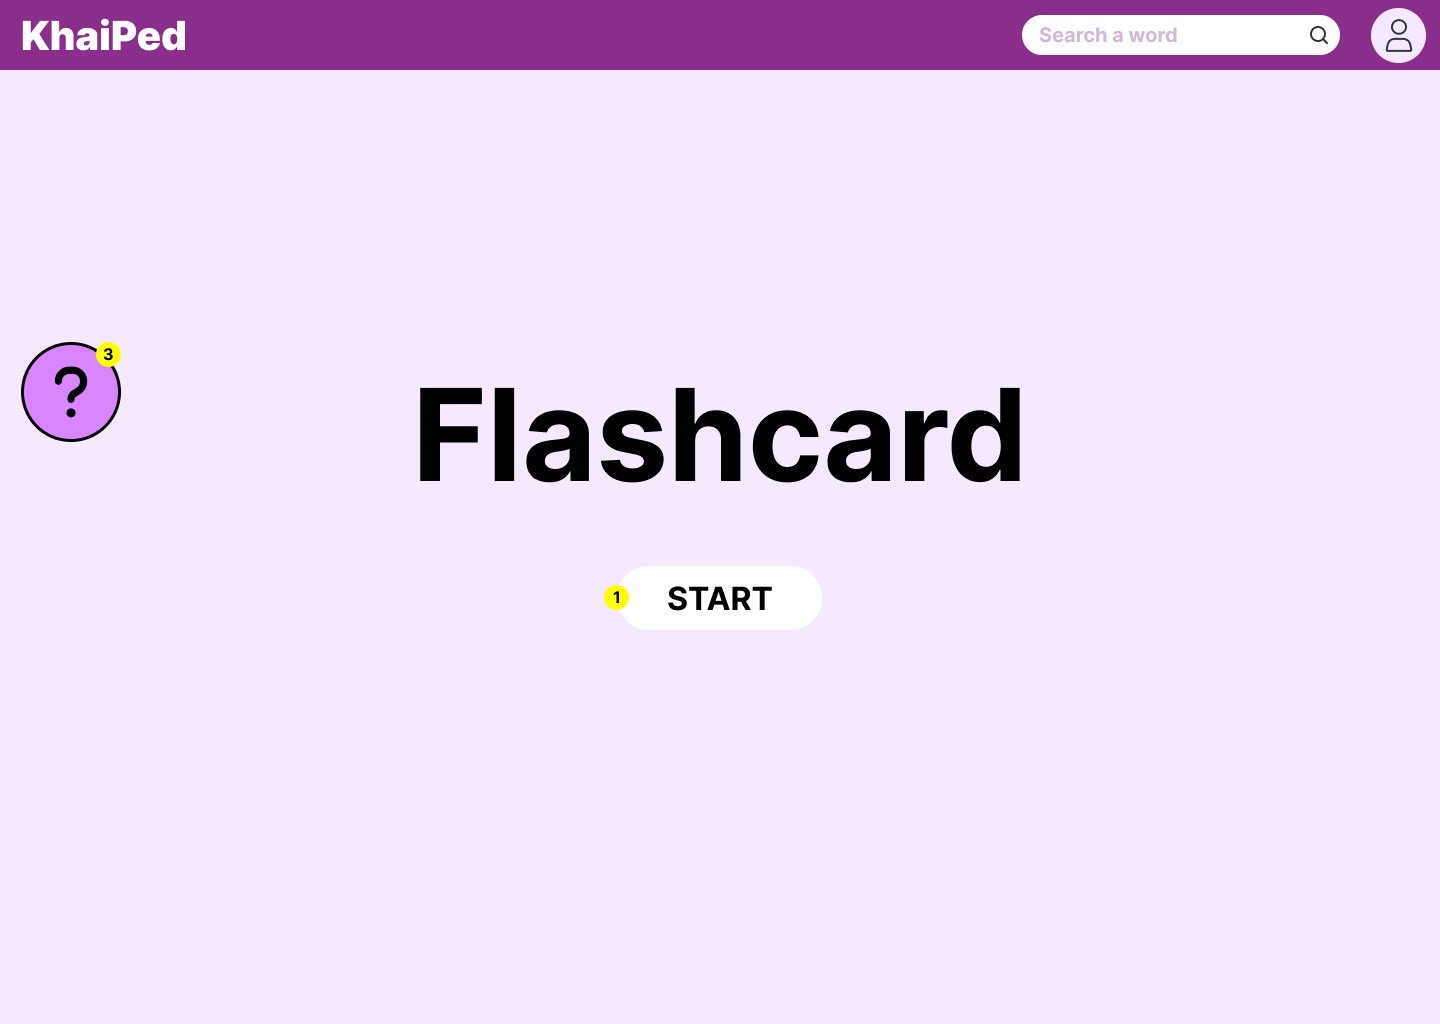
\includegraphics[width=0.8\textwidth, keepaspectratio=true]{image/chap3/ui/flashcard/Flashcard.png}
	\caption{หน้าหลักบัตรคำ}\label{fig:UI_Flashcard}
\end{figure}
\hspace{1cm}
จากรูปภาพที่ \ref{fig:UI_Home} เมื่อผู้ใช้กดปุ่มบัตรคำ ระบบจะแสดงผลหน้าบัตรคำ ซึ่งแสดงให้เห็นดังรูปภาพที่ \ref{fig:UI_Flashcard}
โดยในหน้าจะประกอบไปด้วยปุ่มสองปุ่ม ได้แก่ ปุ่มเริ่มใช้งานบัตรคำ (1) เมื่อกดแล้ว ระบบจะสุ่มคำศัพท์จำนวน 10 คำ
แล้วทำการแสดงผลบัตรคำ และปุ่มช่วยเหลือ (2) โดยเมื่อกดแล้ว ระบบจะแสดงผลวิธีการใช้งานบัตรคำ

\begin{figure}[!h]\centering
	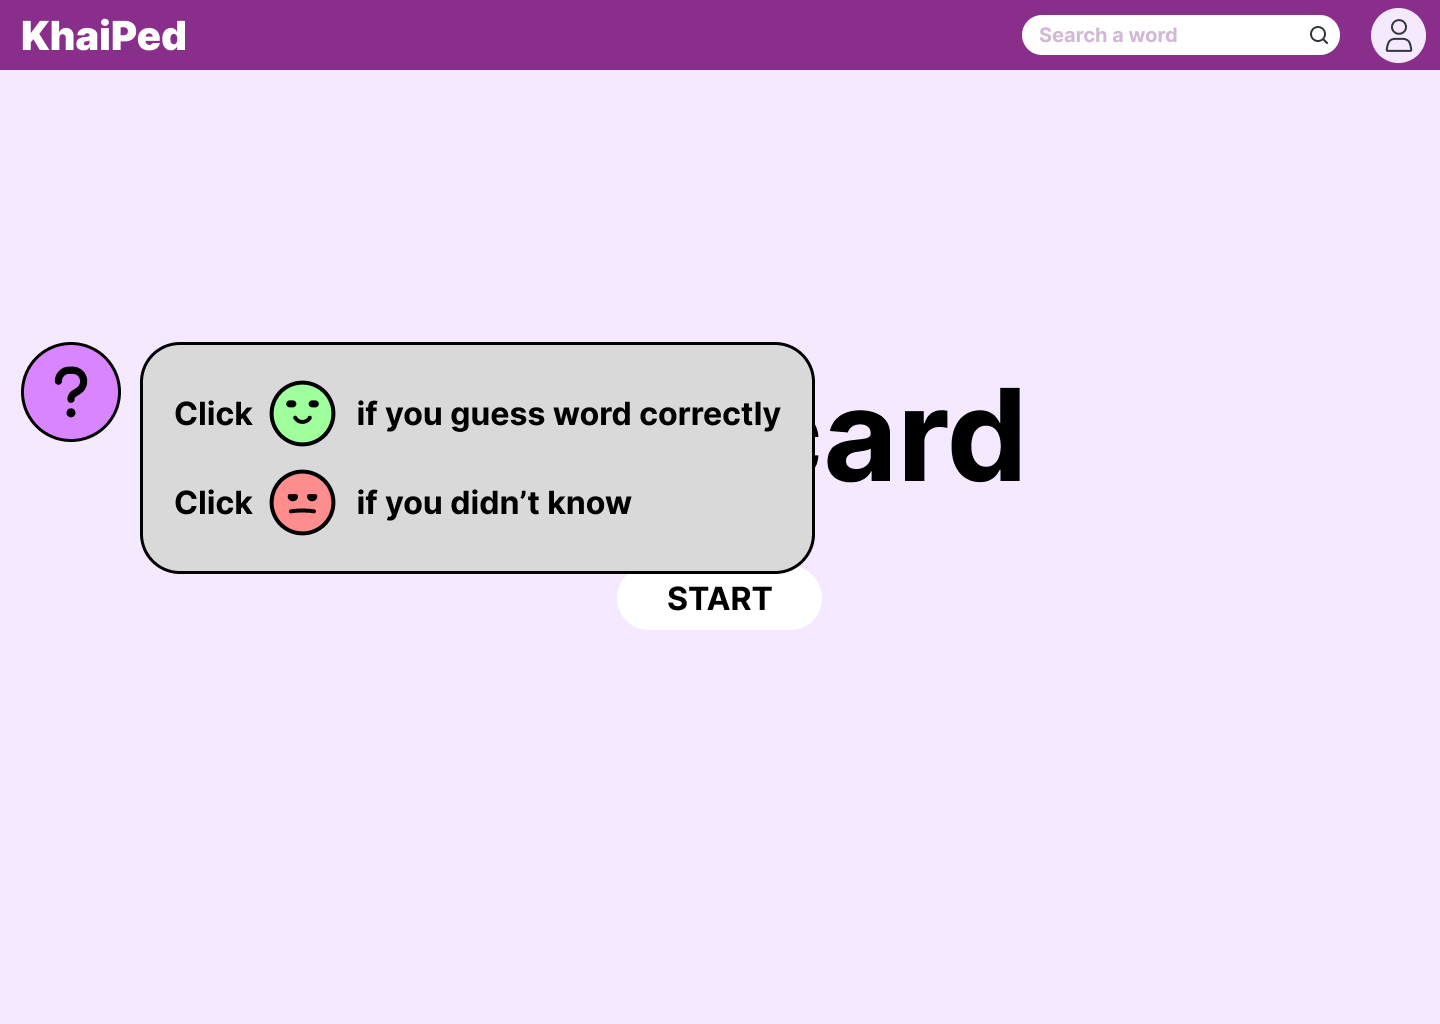
\includegraphics[width=0.8\textwidth, keepaspectratio=true]{image/chap3/ui/flashcard/Flashcard - Help.png}
	\caption{ปุ่มช่วยเหลือหน้าบัตรคำ}\label{fig:UI_FlashcardHelp}
\end{figure}
\hspace{1cm}
จากรูปภาพที่ \ref{fig:UI_Flashcard} เมื่อกดปุ่มช่วยเหลือในหน้าบัตรคำ จะแสดงผลกล่องข้อความที่แสดงวิธีการใช้งานบัตรคำ ซึ่งแสดงให้เห็นดังรูปภาพที่ \ref{fig:UI_FlashcardHelp}

% \begin{figure}[!h]\centering
% 	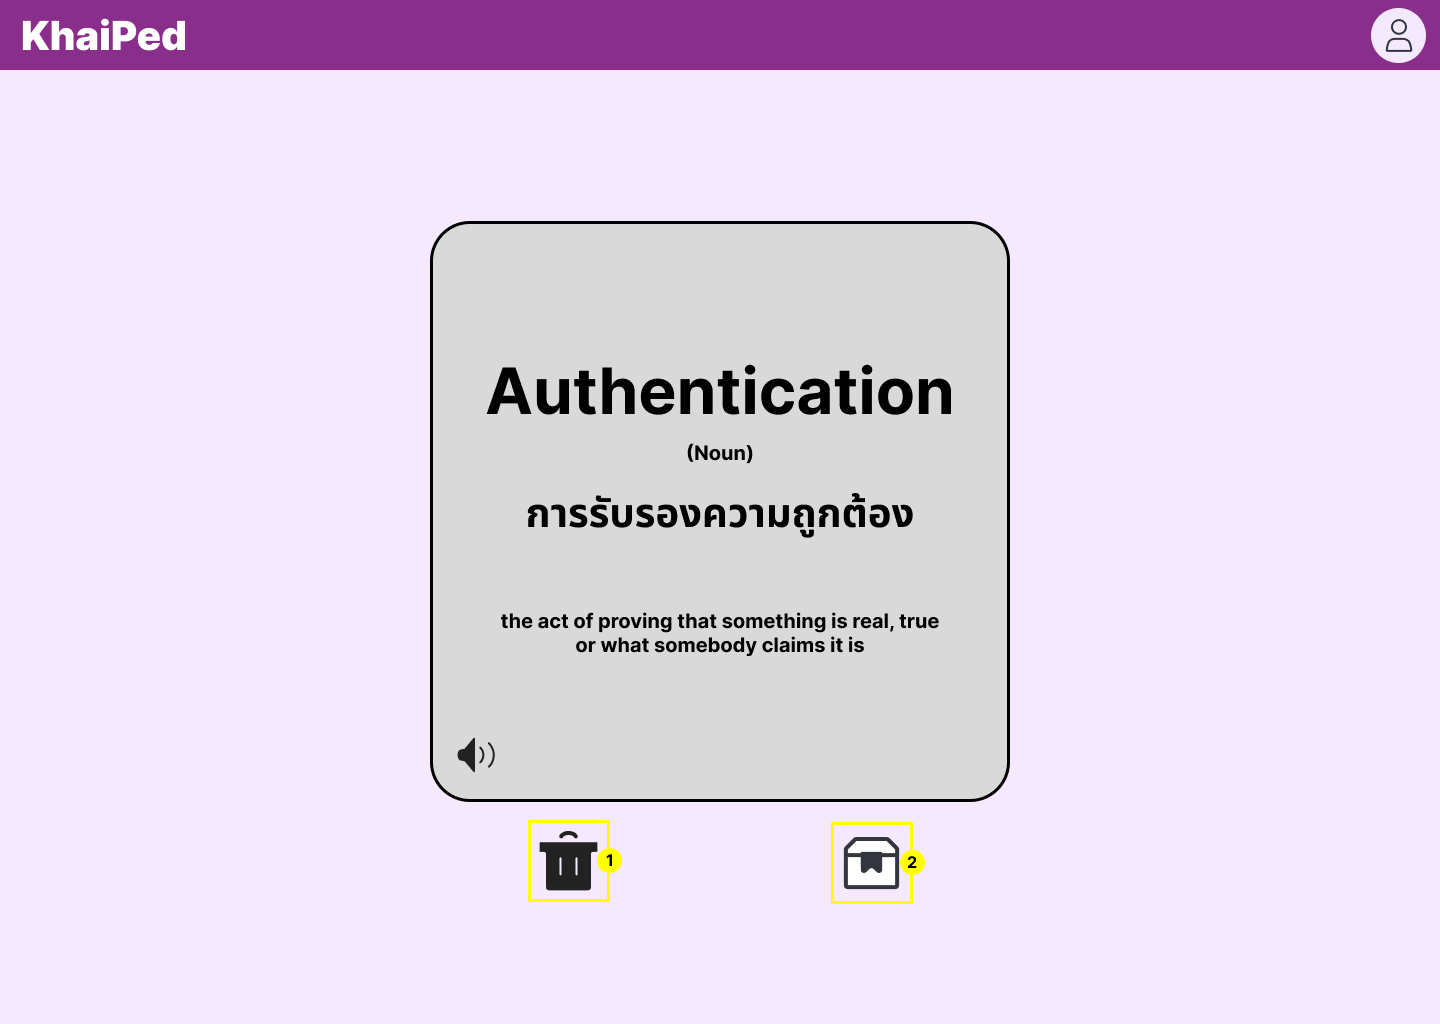
\includegraphics[width=0.8\textwidth, keepaspectratio=true]{image/chap3/ui/flashcard/Flashcard - Select Word.png}
% 	\caption{หน้าเลือกคำศัพท์เพื่อใช้งานบัตรคำ}\label{fig:UI_SelectFlashcard1}
% \end{figure}
% \hspace{1cm}
% จากรูปภาพที่ \ref{fig:UI_Flashcard} เมื่อผู้ใช้กดปุ่มเลือกคำศัพท์ ระบบจะแสดงการ์ดคำศัพท์ ดังรูปภาพที่ \ref{fig:UI_SelectFlashcard1}
% ซึ่งจะมีรายละเอียดของคำศัพท์อยู่บนการ์ด โดยจะมีปุ่มเล่นเสียง ปุ่มทิ้งคำศัพท์ (1)
% เมื่อกดแล้วระบบจะสุ่มคำศัพท์ใหม่มาแสดงผลให้ผู้ใช้เลือก และปุ่มเก็บคำศัพท์ (2) เมื่อกดแล้วระบบจะเก็บคำศัพท์ที่เลือกแล้วแสดงผลคำศัพท์ใหม่

% \pagebreak
% \begin{figure}[!h]\centering
% 	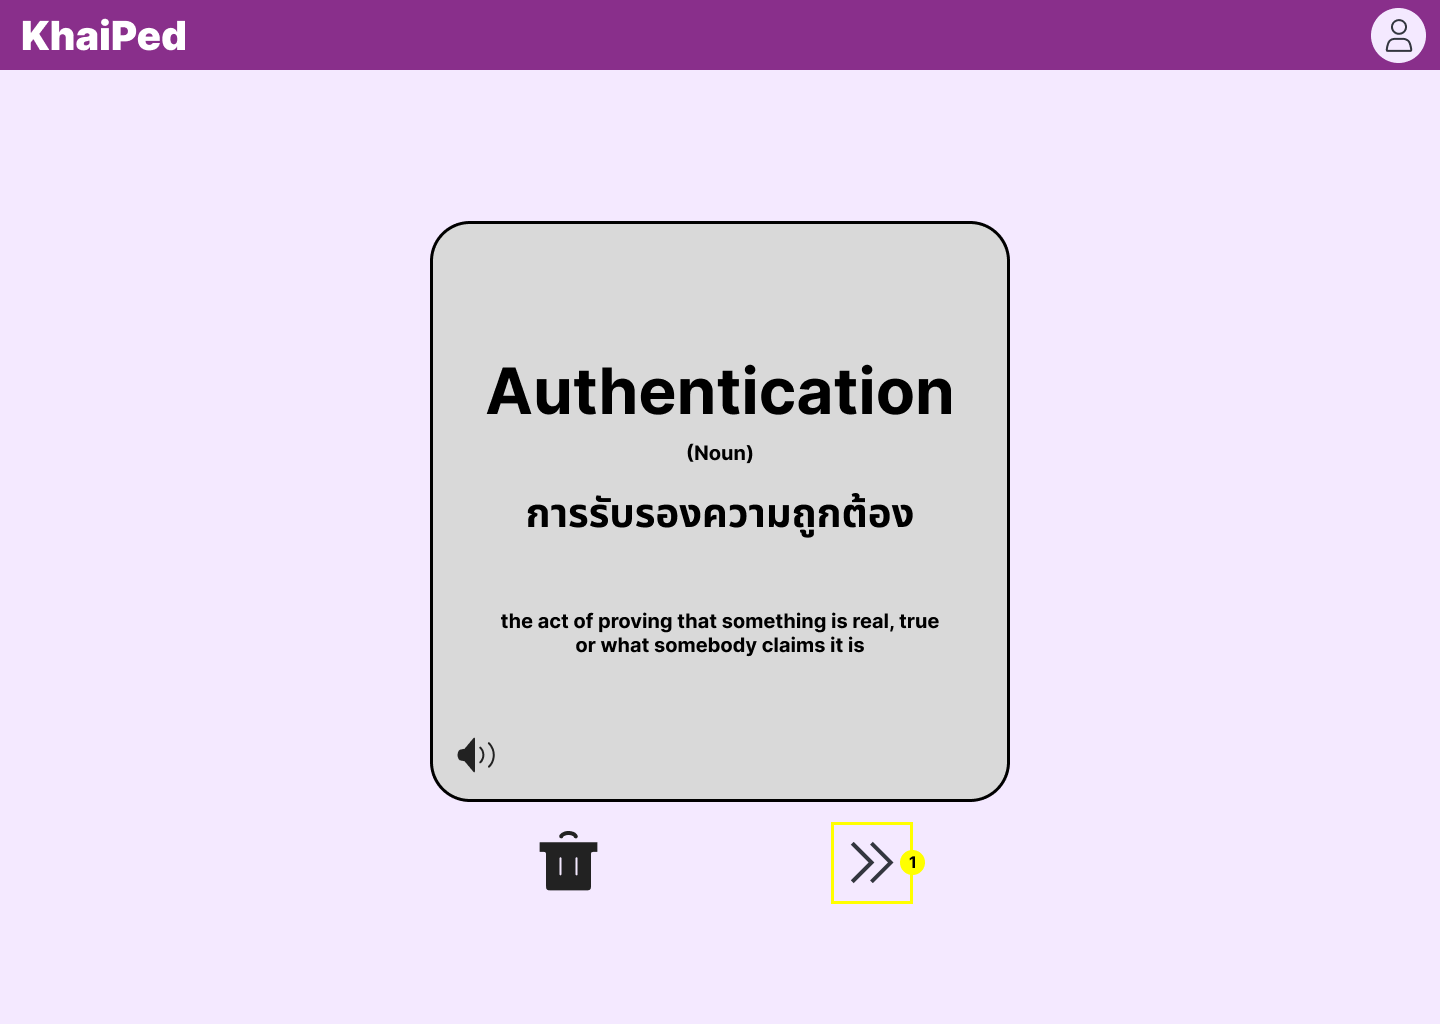
\includegraphics[width=0.8\textwidth, keepaspectratio=true]{image/chap3/ui/flashcard/Flashcard - Select Word-1.png}
% 	\caption{เมื่อเลือกคำศัพท์เพื่อใช้งานบัตรคำครบแล้ว}\label{fig:UI_SelectFlashcard2}
% \end{figure}
% \hspace{1cm}
% จากรูปภาพที่ \ref{fig:UI_SelectFlashcard1} เมื่อผู้ใช้กดปุ่มเก็บคำศัพท์จนระบบเก็บคำศัพท์ครบ 10 คำแล้ว
% ปุ่มเก็บคำศัพท์จะเปลี่ยนเป็นปุ่มถัดไป (1) เมื่อกดแล้วระบบจะแสดงผลบัตรคำที่เก็บไว้ ดังรูปภาพที่ \ref{fig:UI_SelectFlashcard2}

\pagebreak
\begin{figure}[!h]\centering
	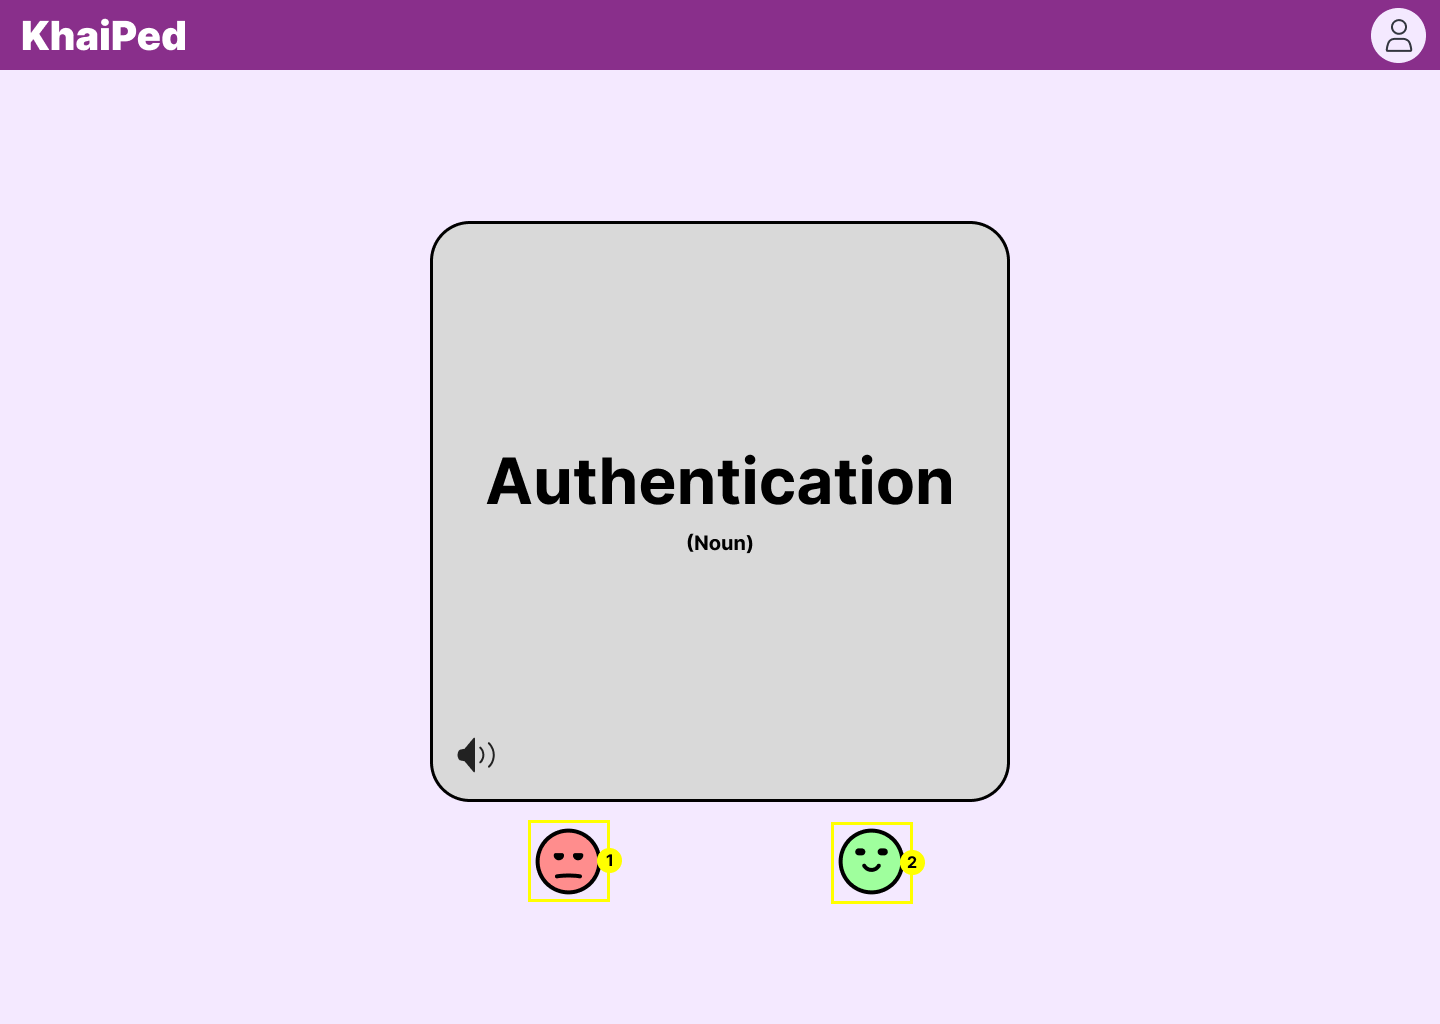
\includegraphics[width=0.8\textwidth, keepaspectratio=true]{image/chap3/ui/flashcard/Flashcard - Show Card.png}
	\caption{หน้าแสดงผลด้านหน้าบัตรคำ}\label{fig:UI_ShowCard}
\end{figure}
\hspace{1cm}
จากรูปภาพที่ \ref{fig:UI_Flashcard} เมื่อผู้ใช้กดปุ่มเริ่มใช้งานบัตรคำในหน้าบัตรคำ ระบบจะแสดงผลบัตรคำ ดังรูปภาพที่ \ref{fig:UI_ShowCard} โดยด้านหน้าของบัตรคำจะมีเพียงคำศัพท์ และ Part of Speech เมื่อผู้ใช้กดที่บัตรคำ
ระบบจะแสดงผลด้านหลังของบัตรคำ และผู้ใช้ยังสามารถกดปุ่มจำคำศัพท์ไม่ได้ (1) เมื่อกดแล้วระบบจะเก็บคำศัพท์นี้ไว้ และแสดงผลคำศัพท์ถัดไป และปุ่มจำศัพท์ได้ (2)
เมื่อกดแล้วระบบจะลบคำศัพท์ และแสดงผลคำศัพท์ถัดไป

\begin{figure}[!h]\centering
	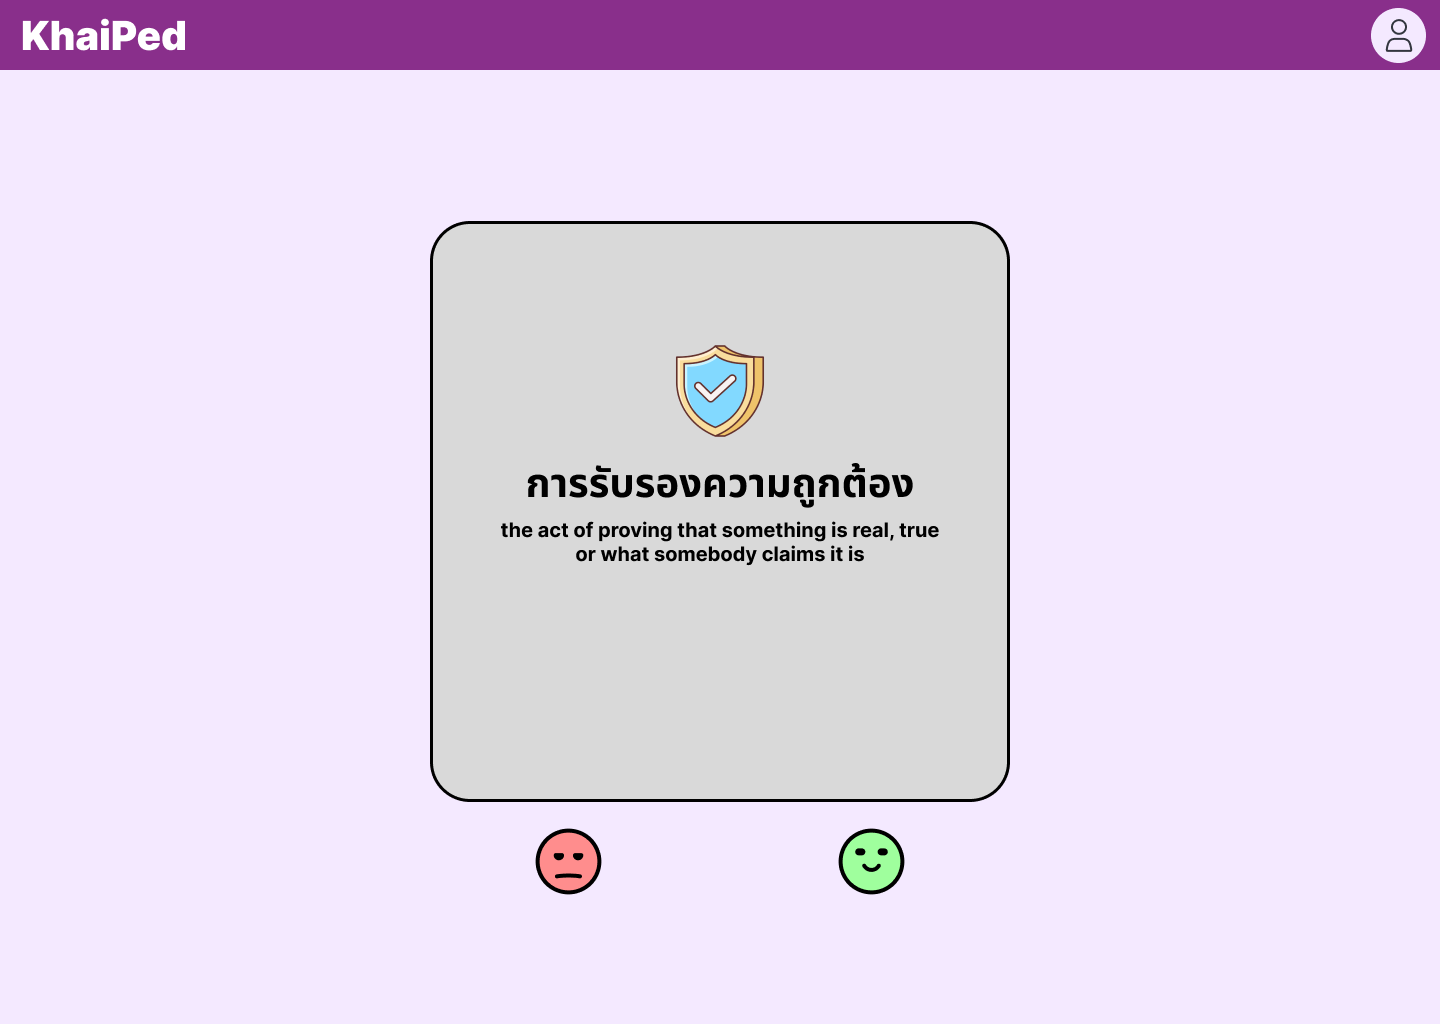
\includegraphics[width=0.8\textwidth, keepaspectratio=true]{image/chap3/ui/flashcard/Flashcard - Flip Card.png}
	\caption{หน้าแสดงผลด้านหลังบัตรคำ}\label{fig:UI_FlipCard}
\end{figure}
\hspace{1cm}
เมื่อผู้ใช้กดบัตรคำด้านหน้า ระบบจะแสดงผลบัตรคำด้านหลัง ซึ่งประกอบไปด้วยรูปภาพ และความหมายทั้งภาษาไทยและภาษาอังกฤษ ดังรูปภาพที่ \ref{fig:UI_FlipCard}

\pagebreak
\begin{figure}[!h]\centering
	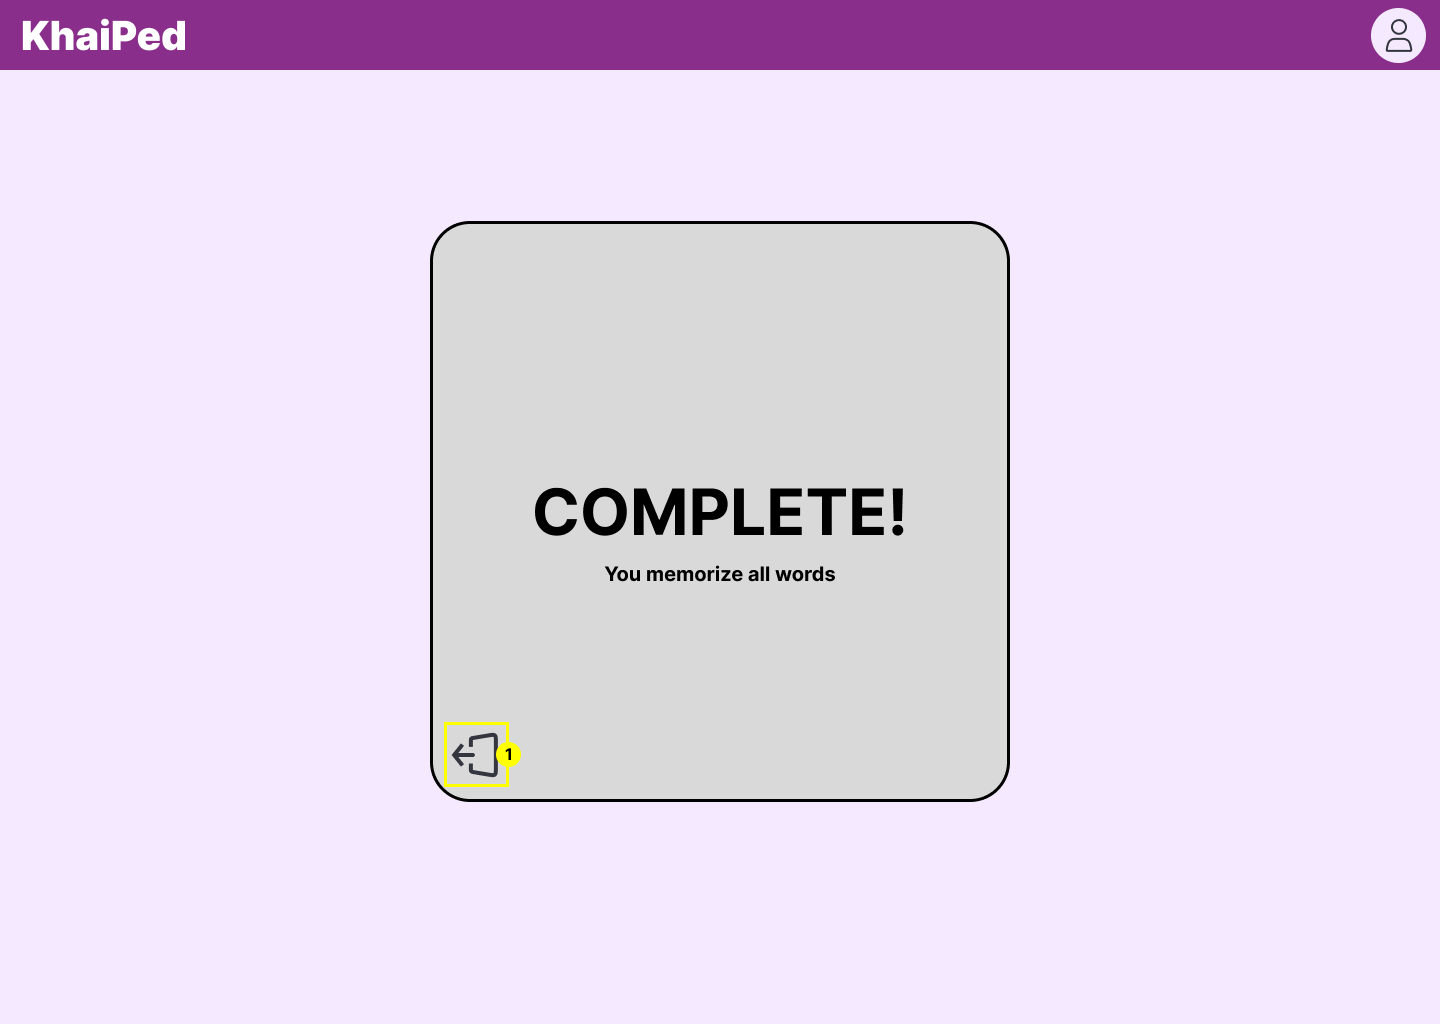
\includegraphics[width=0.8\textwidth, keepaspectratio=true]{image/chap3/ui/flashcard/Flashcard - Complete.png}
	\caption{หน้าแสดงผลลัพธ์การใช้บัตรคำ}\label{fig:UI_FlashcardResult}
\end{figure}
\hspace{1cm}
เมื่อผู้ใช้กดปุ่มจำศัพท์ได้จนไม่เหลือคำศัพท์แล้ว ระบบจะแสดงผลว่าผู้ใช้จำศัพท์ได้ครบแล้ว และสามารถกดปุ่มออก (1) เพื่อกลับไปหน้าหลักได้ ซึ่งแสดงให้เห็นดังรูปภาพที่ \ref{fig:UI_FlashcardResult}

\pagebreak
\subsection{เกมเรียงพยัญชนะเป็นคำศัพท์}
\begin{figure}[!h]\centering
	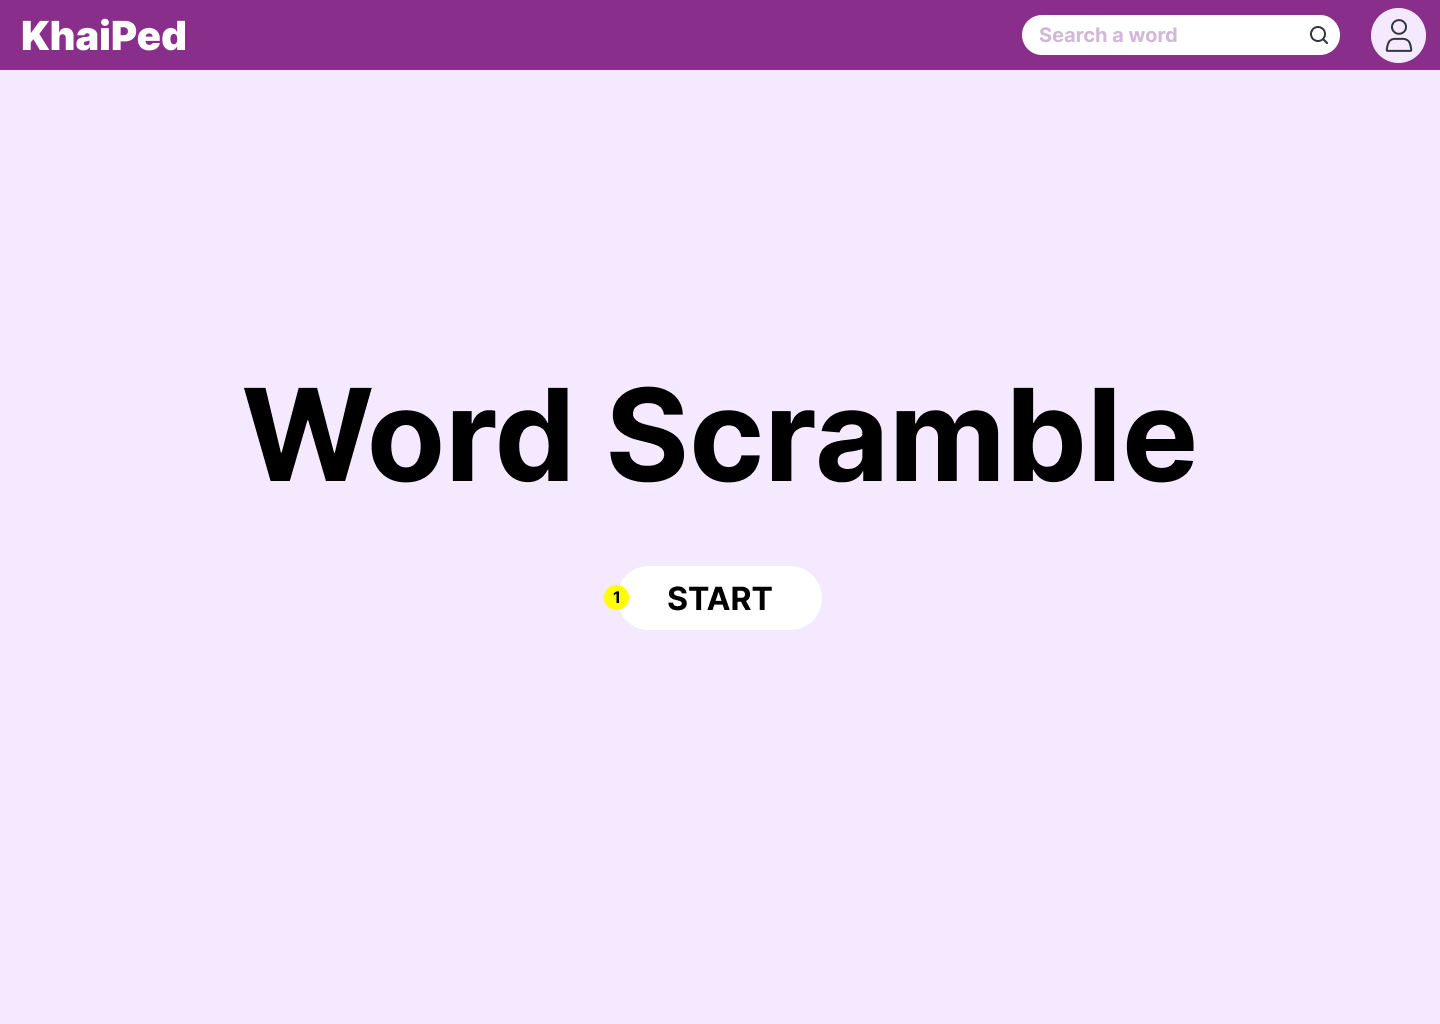
\includegraphics[width=0.8\textwidth, keepaspectratio=true]{image/chap3/ui/game/Word Scramble.png}
	\caption{หน้าหลักของการเล่นเกมเรียงพยัญชนะเป็นคำศัพท์}\label{fig:UI_Game}
\end{figure}
\hspace{1cm}
จากรูปภาพที่ \ref{fig:UI_Home} เมื่อผู้ใช้กดปุ่มเล่นเกม ระบบจะแสดงผลหน้าหลักของการเล่นเกม ซึ่งแสดงให้เห็นดังรูปภาพที่ \ref{fig:UI_Game} โดยในหน้าจะประกอบไปด้วย
ปุ่มเริ่มเล่นเกม (1) เมื่อกดแล้ว ระบบจะทำการสุ่มคำศัพท์และแสดงผลหน้าสำหรับเล่นเกม และปุ่มช่วยเหลือ (2) โดยเมื่อกดแล้ว ระบบจะแสดงผลวิธีการเล่นเกม

\begin{figure}[!h]\centering
	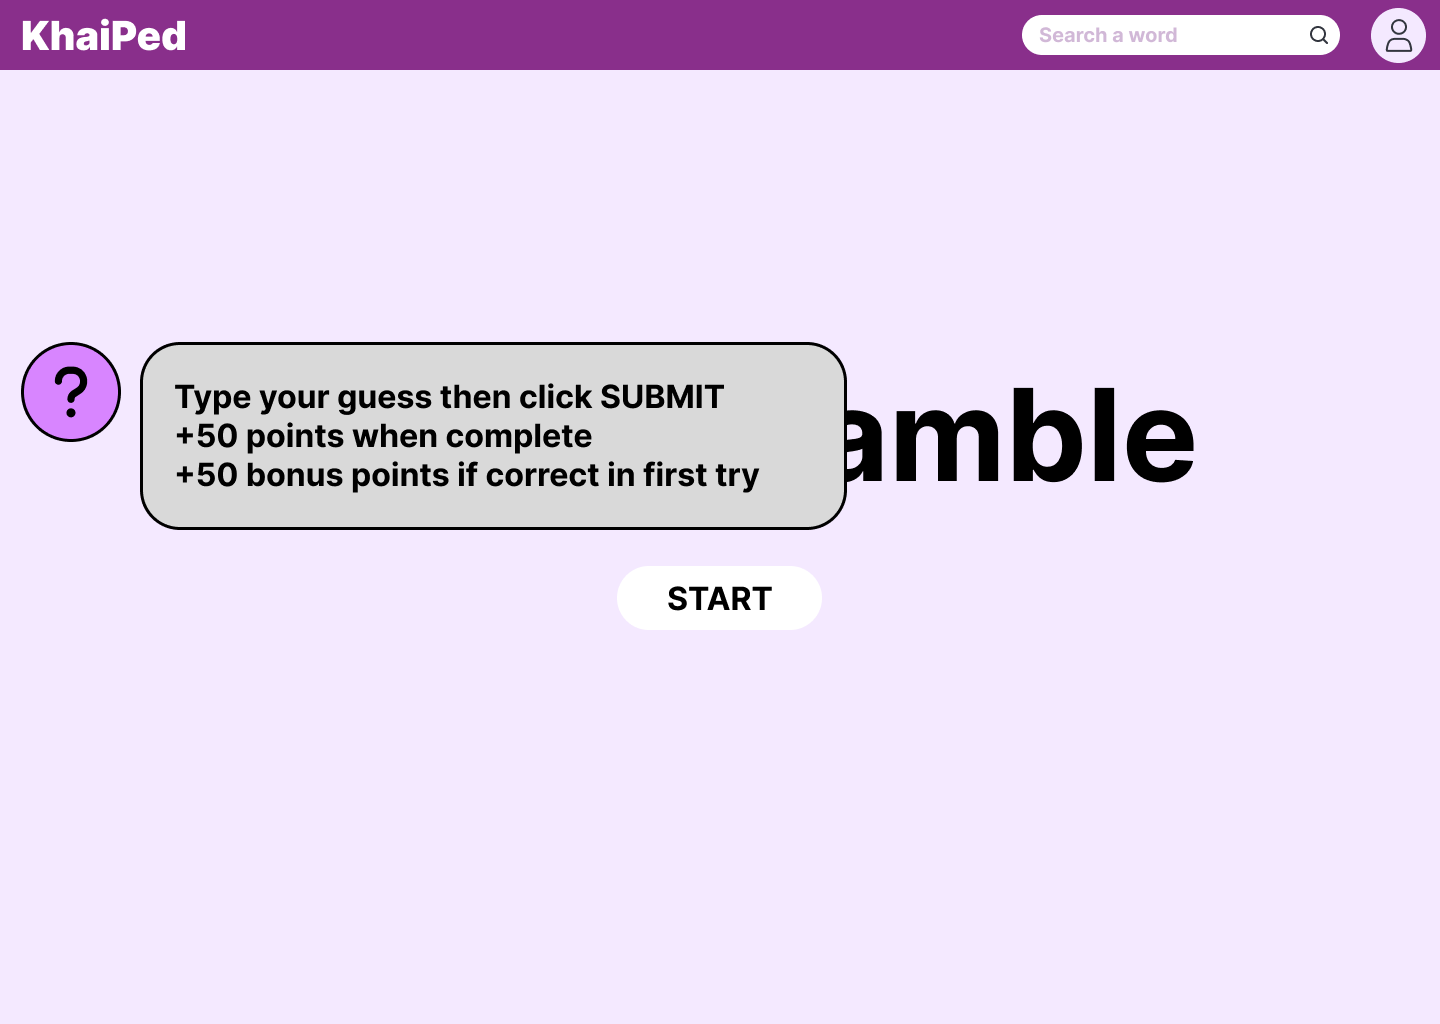
\includegraphics[width=0.8\textwidth, keepaspectratio=true]{image/chap3/ui/game/Word Scramble - Help.png}
	\caption{ปุ่มช่วยเหลือหน้าเล่นเกม}\label{fig:UI_GameHelp}
\end{figure}
\hspace{1cm}
จากรูปภาพที่ \ref{fig:UI_Game} เมื่อกดปุ่มช่วยเหลือในหน้าเล่นเกม จะแสดงผลกล่องข้อความที่แสดงวิธีการเล่นเกม ซึ่งแสดงให้เห็นดังรูปภาพที่ \ref{fig:UI_GameHelp}

\pagebreak
\begin{figure}[!h]\centering
	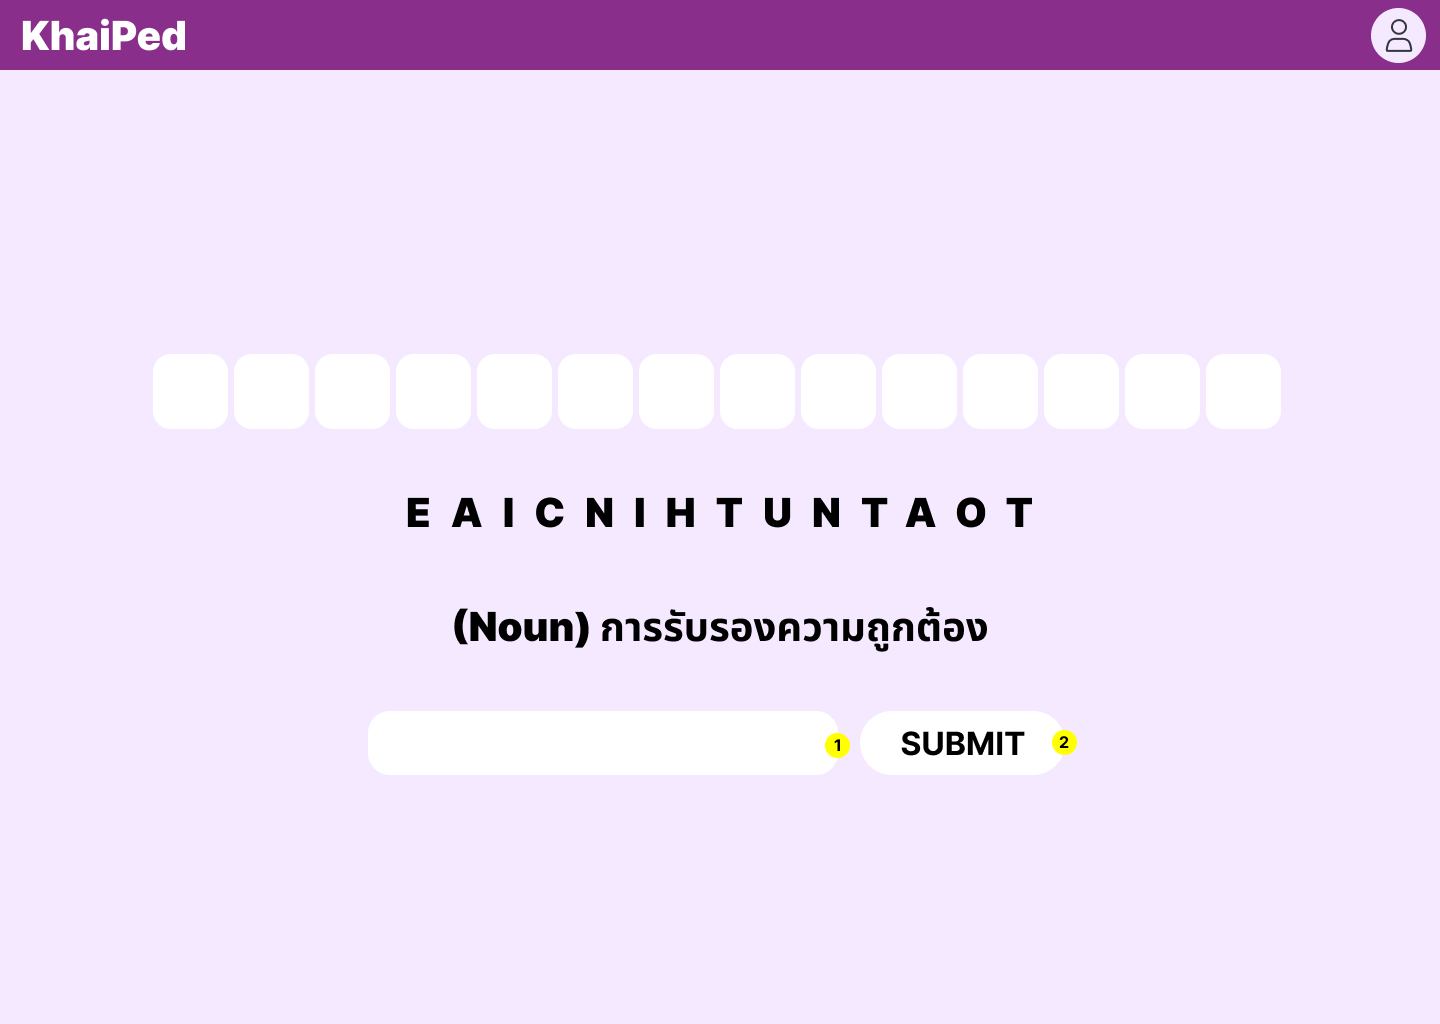
\includegraphics[width=0.8\textwidth, keepaspectratio=true]{image/chap3/ui/game/Word Scramble - Start.png}
	\caption{หน้าเล่นเกมเรียงพยัญชนะเป็นคำศัพท์}\label{fig:UI_StartGame}
\end{figure}
\hspace{1cm}
จากรูปภาพที่ \ref{fig:UI_Game} เมื่อผู้ใช้กดปุ่มปุ่มเริ่มเล่นเกม ระบบจะแสดงผลหน้าเล่นเกม ดังรูปภาพที่ \ref{fig:UI_StartGame}
โดยจะประกอบไปด้วยกล่องตัวอักษร สำหรับแสดงผลตัวอักษรที่ผู้ใช้ใส่ ตัวอักษรที่ถูกสลับที่
และความหมายของคำ ช่องใส่คำศัพท์ (1) สำหรับให้ผู้ใช้กรอกคำศัพท์ และปุ่มส่งคำศัพท์ (2) เมื่อกดแล้วระบบจะตรวจสอบว่าตัวอักษรที่ผู้ใช้ใส่ถูกตำแหน่งหรือไม่

\begin{figure}[!h]\centering
	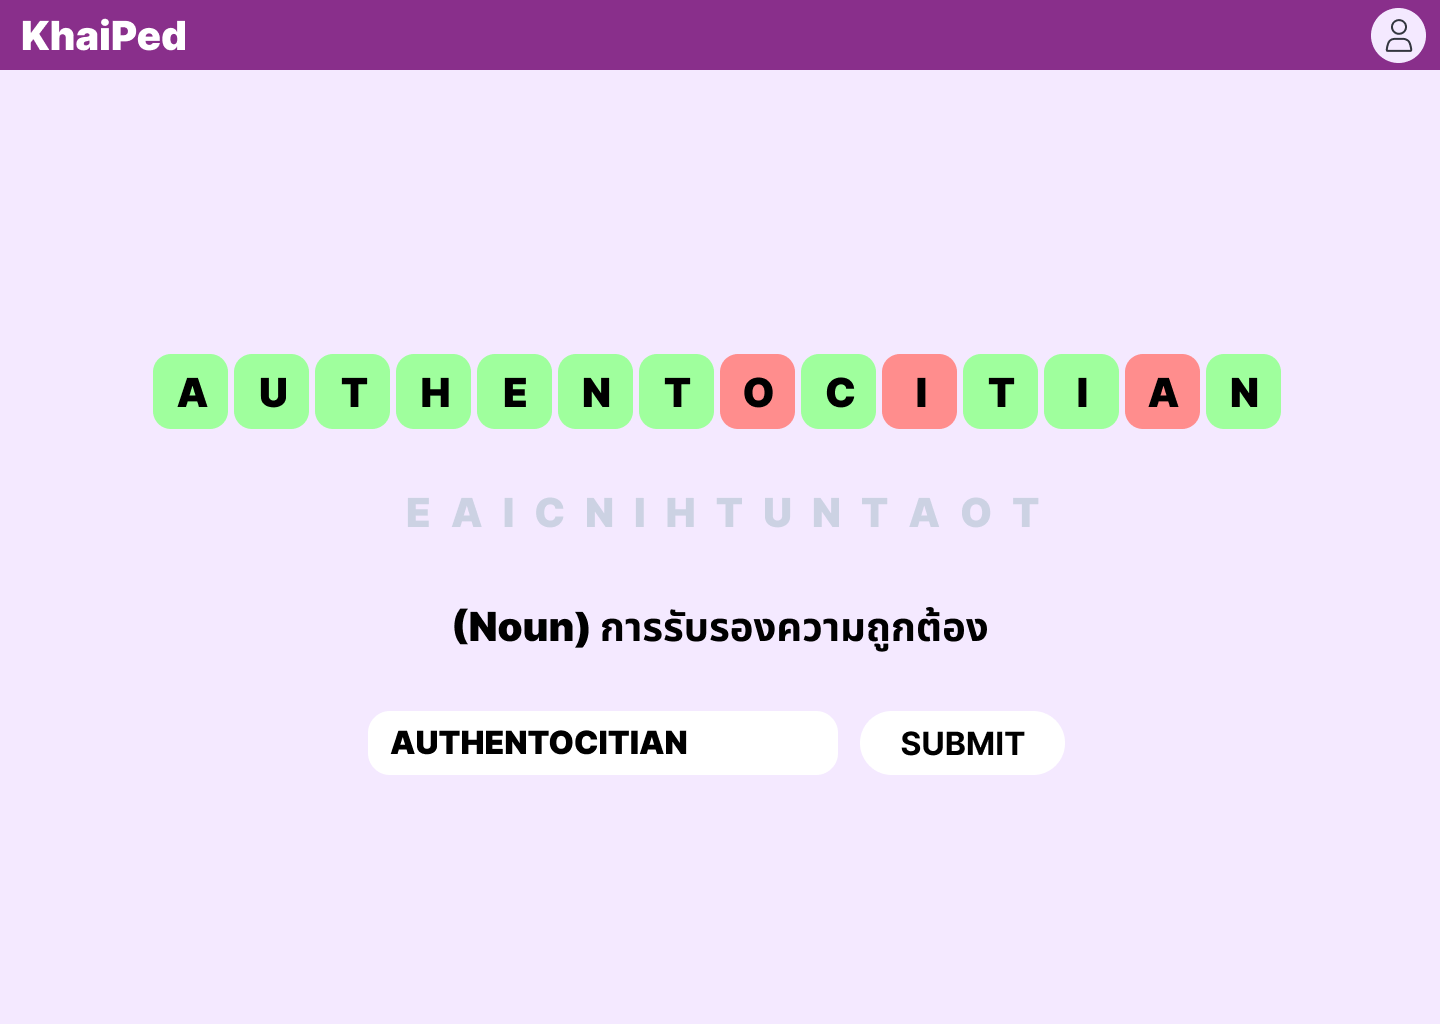
\includegraphics[width=0.8\textwidth, keepaspectratio=true]{image/chap3/ui/game/Word Scramble - Wrong Answer.png}
	\caption{การแสดงผลหากใส่คำตอบผิด}\label{fig:UI_GameWrong}
\end{figure}
\hspace{1cm}
หากผู้ใช้ใส่พยัญชนะผิดตำแหน่งและกดปุ่มส่งคำศัพท์ ระบบจะตรวจสอบว่าตัวอักษรที่ผู้ใช้ใส่ถูกตำแหน่งหรือไม่ และจะแสดงผลพยัญชนะที่อยู่ในตำแหน่งถูก และผิด
ซึ่งแสดงให้เห็นดังรูปภาพที่ \ref{fig:UI_GameWrong}

\pagebreak
\begin{figure}[!h]\centering
	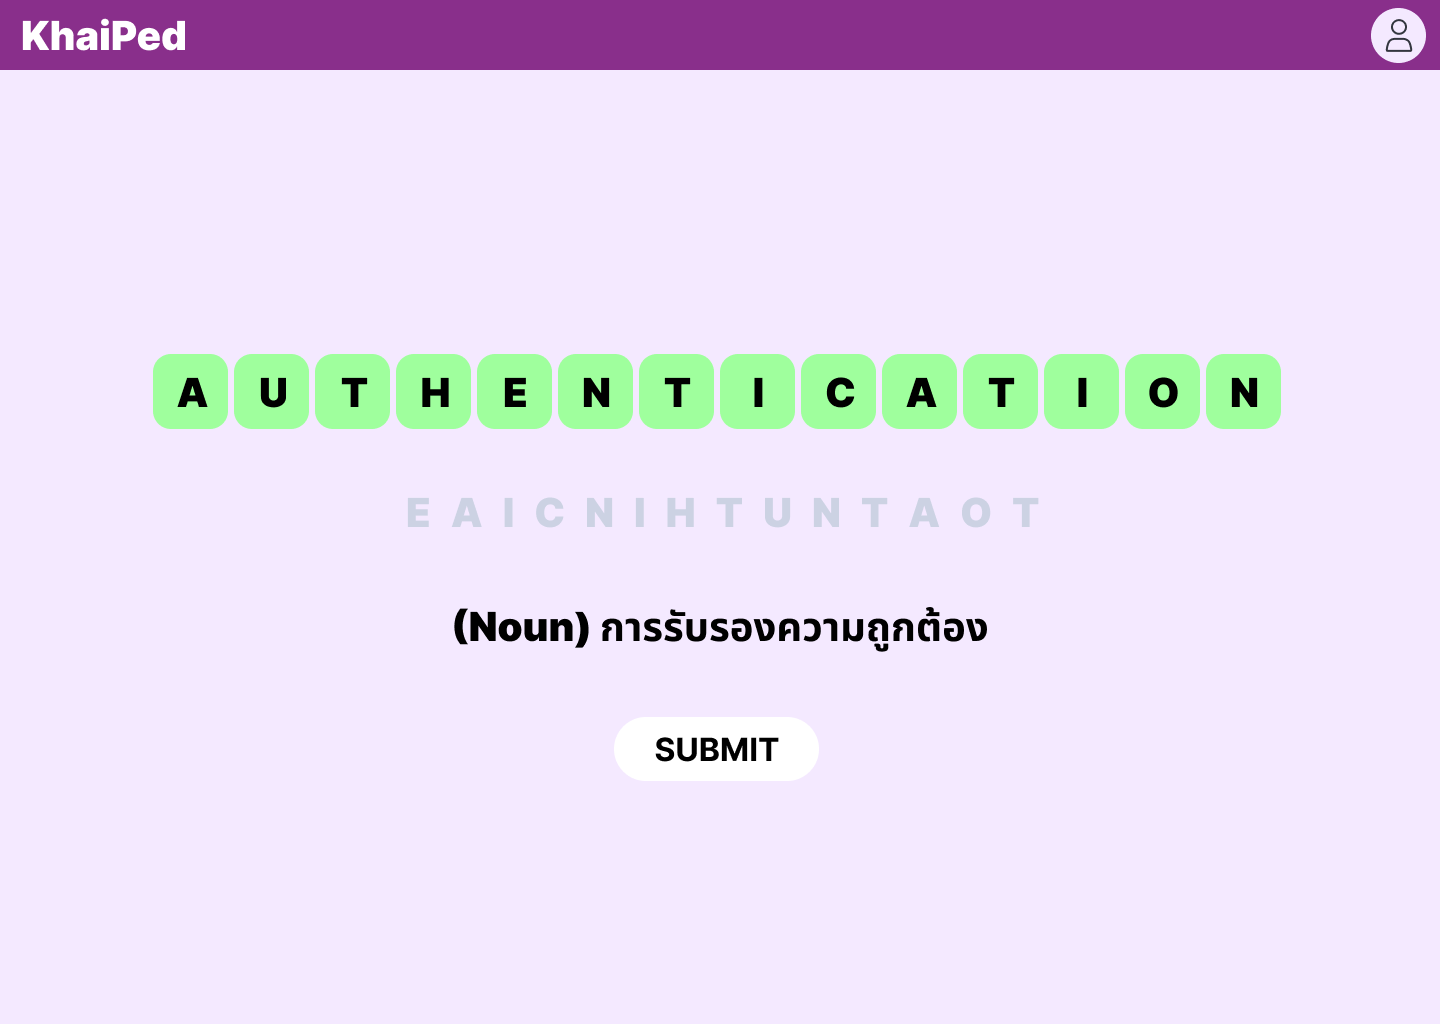
\includegraphics[width=0.8\textwidth, keepaspectratio=true]{image/chap3/ui/game/Word Scramble - Correct Answer.png}
	\caption{การแสดงผลหากใส่คำตอบถูก}\label{fig:UI_GameCorrect}
\end{figure}
\hspace{1cm}
หากผู้ใช้ใส่พยัญชนะถูกทุกตำแหน่งและกดปุ่มส่งคำศัพท์ ระบบจะตรวจสอบว่าตัวอักษรที่ผู้ใช้ใส่ถูกตำแหน่งหรือไม่ และจะแสดงผลพยัญชนะที่อยู่ในตำแหน่งถูก
ซึ่งแสดงให้เห็นดังรูปภาพที่ \ref{fig:UI_GameCorrect}

\begin{figure}[!h]\centering
	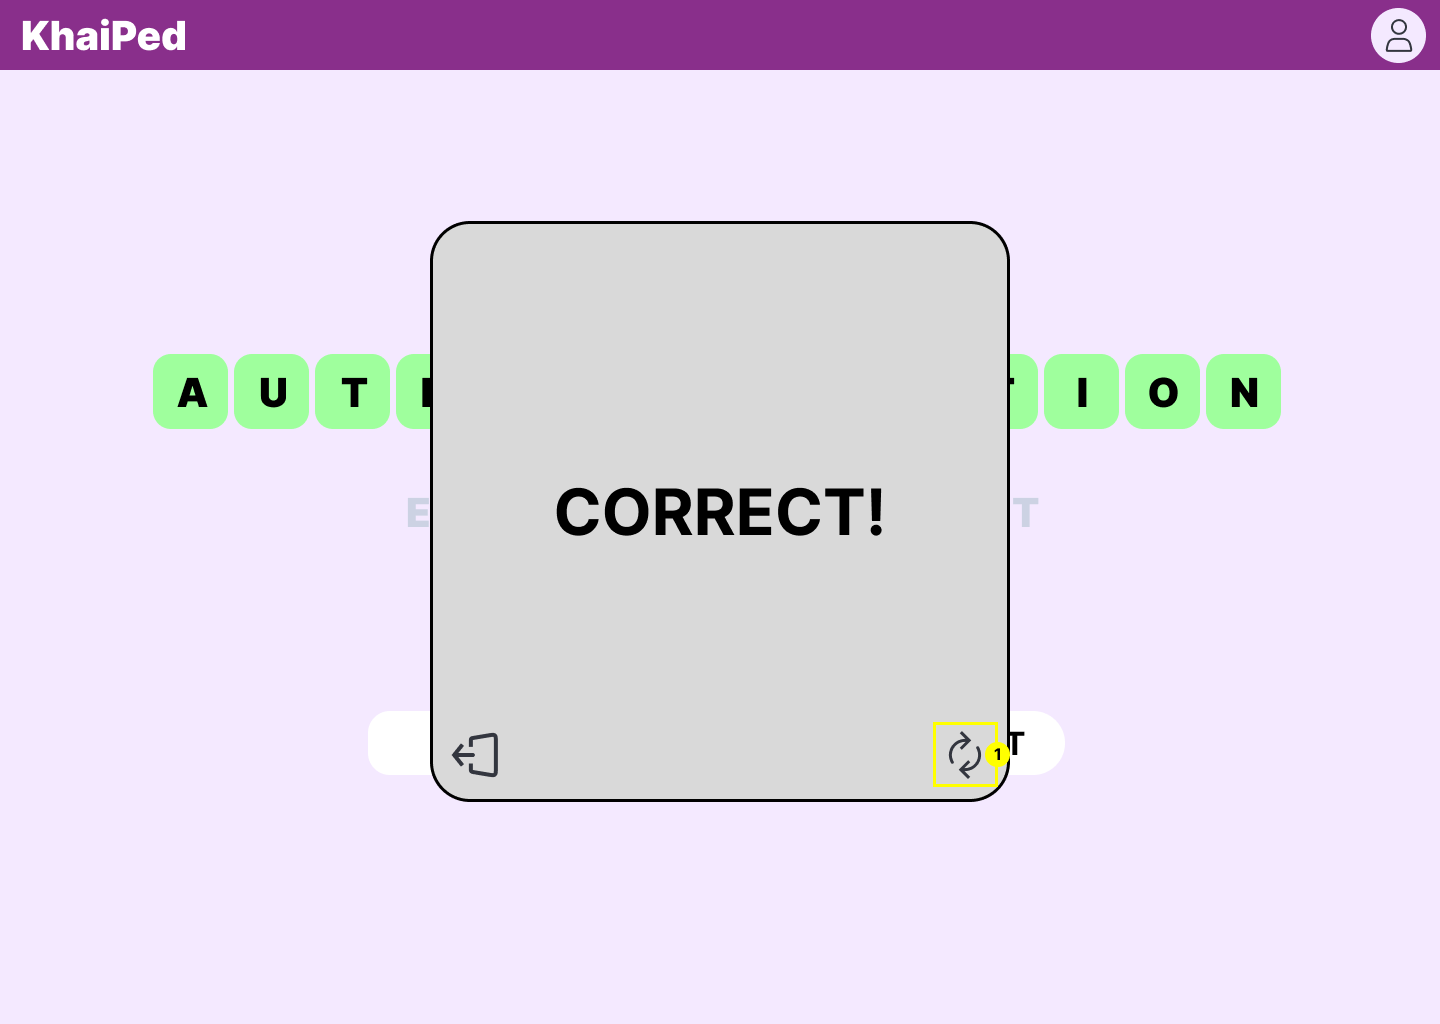
\includegraphics[width=0.8\textwidth, keepaspectratio=true]{image/chap3/ui/game/Word Scramble - Pop Up.png}
	\caption{การแสดงผลลัพท์การเล่นเกม}\label{fig:UI_GameResult}
\end{figure}
\hspace{1cm}
เมื่อผู้ใช้เรียงคำศัพท์ได้ถูกต้องแล้วกดปุ่มส่งคำศัพท์ หลังจากที่ระบบแสดงผลพยัญชนะที่อยู่ในตำแหน่งถูกแล้ว ระบบจะแสดงผลว่าผู้ใช้เรียงคำศัพท์ได้ถูกต้อง
ซึ่งแสดงให้เห็นดังรูปภาพที่ \ref{fig:UI_GameResult}
และสามารถกดปุ่มออกเพื่อกลับไปหน้าหลัก หรือกดปุ่มสุ่มคำใหม่ (1) เพื่อให้ระบบจะสุ่มคำศัพท์ใหม่มาเล่นเกมต่อได้

\pagebreak
\subsection{การทำแบบทดสอบ}
\begin{figure}[!h]\centering
	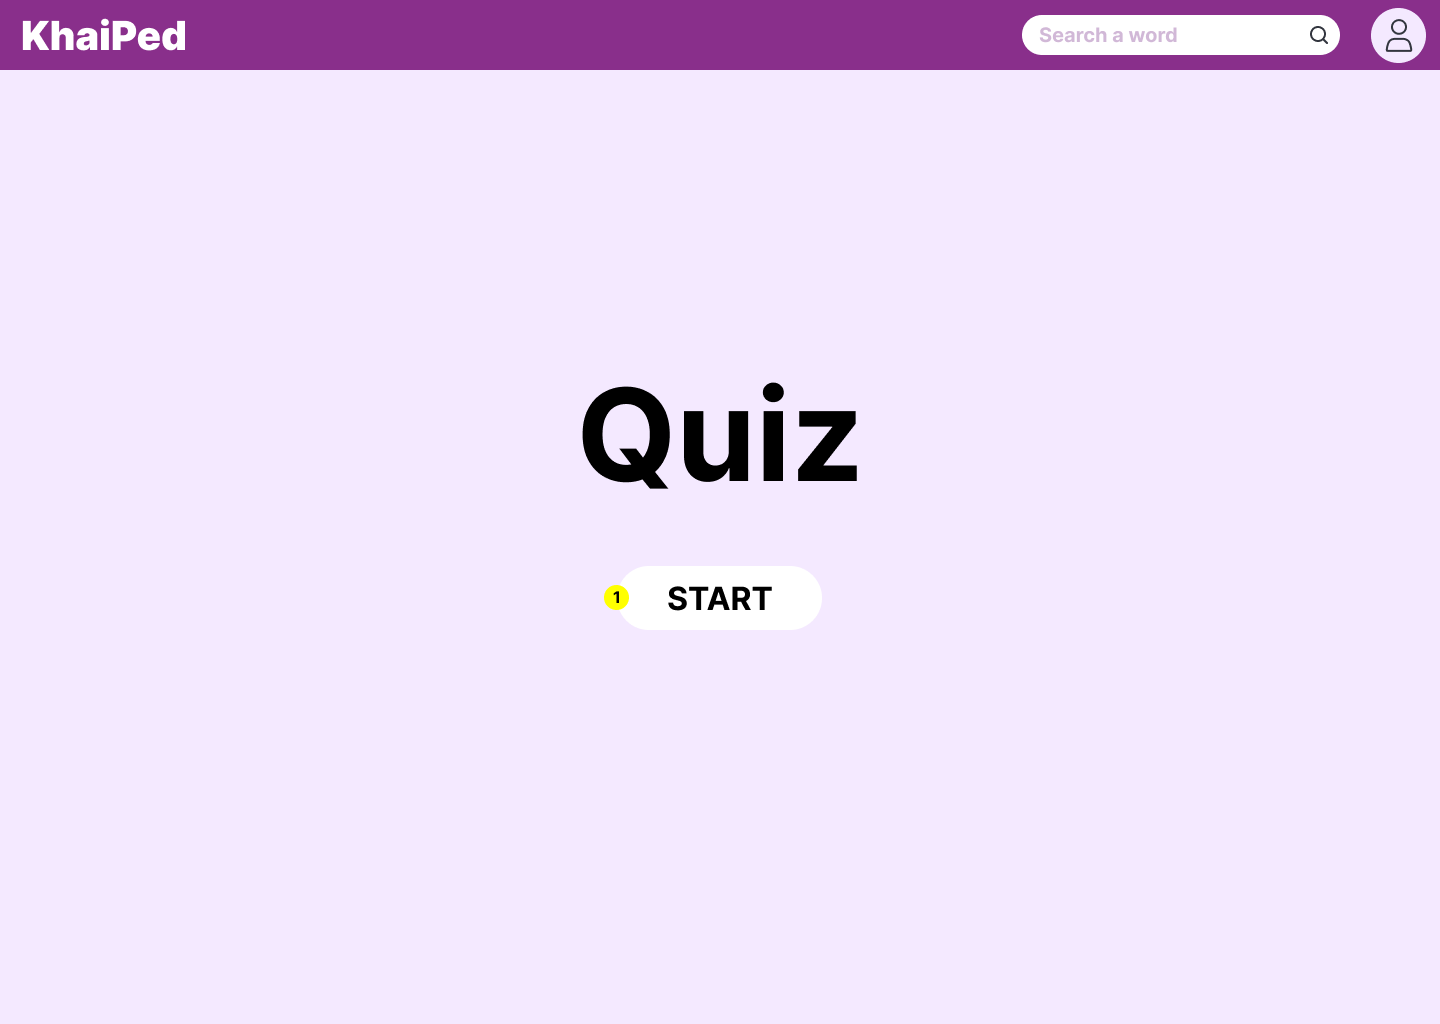
\includegraphics[width=0.8\textwidth, keepaspectratio=true]{image/chap3/ui/quiz/Quiz.png}
	\caption{หน้าหลักของการทำแบบทดสอบ}\label{fig:UI_Quiz}
\end{figure}
\hspace{1cm}
จากรูปภาพที่ \ref{fig:UI_Home} เมื่อผู้ใช้กดปุ่มทำแบบทดสอบ ระบบจะแสดงผลหน้าหลักของการทำแบบทดสอบ ซึ่งแสดงให้เห็นดังรูปภาพที่ \ref{fig:UI_Quiz}
โดยในหน้าจะประกอบไปด้วยปุ่มเริ่มทำแบบทดสอบ (1) เมื่อกดแล้ว ระบบจะทำการสุ่มคำศัพท์ 10 คำและแสดงผลหน้าสำหรับทำแบบทดสอบ
และปุ่มช่วยเหลือ (2) โดยเมื่อกดแล้ว ระบบจะแสดงผลวิธีการทำแบบทดสอบ

\begin{figure}[!h]\centering
	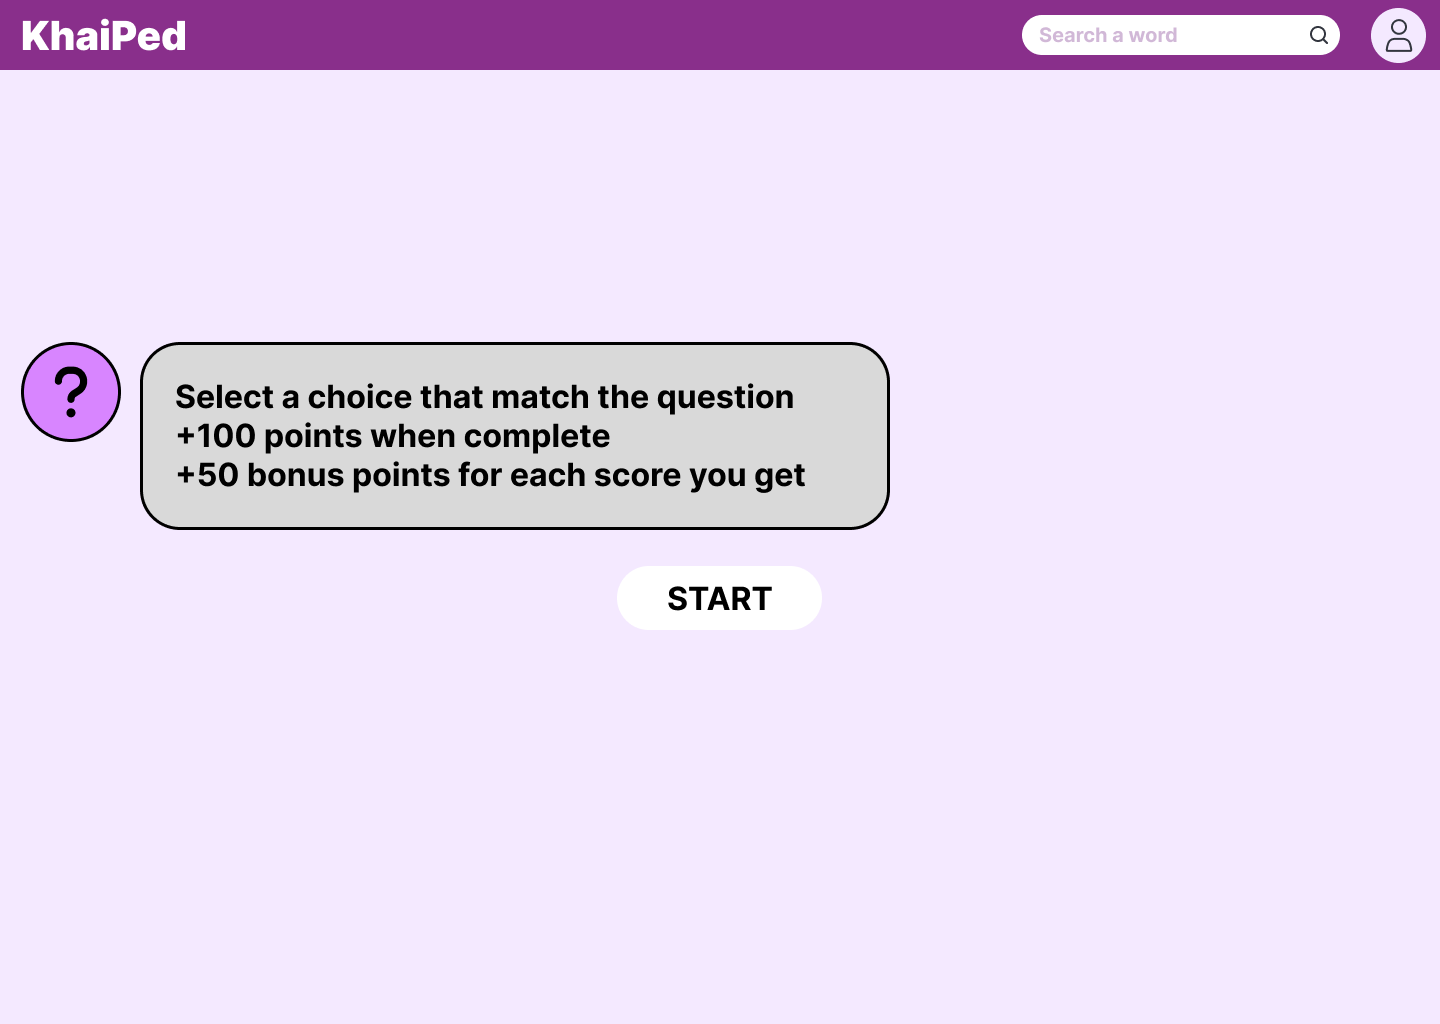
\includegraphics[width=0.8\textwidth, keepaspectratio=true]{image/chap3/ui/quiz/Quiz - Help.png}
	\caption{ปุ่มช่วยเหลือหน้าทำแบบทดสอบ}\label{fig:UI_QuizHelp}
\end{figure}
\hspace{1cm}
จากรูปภาพที่ \ref{fig:UI_Quiz} เมื่อกดปุ่มช่วยเหลือในหน้าทำแบบทดสอบ จะแสดงผลกล่องข้อความที่แสดงวิธีการเทำแบบทดสอบ ซึ่งแสดงให้เห็นดังรูปภาพที่ \ref{fig:UI_QuizHelp}

\pagebreak
\begin{figure}[!h]\centering
	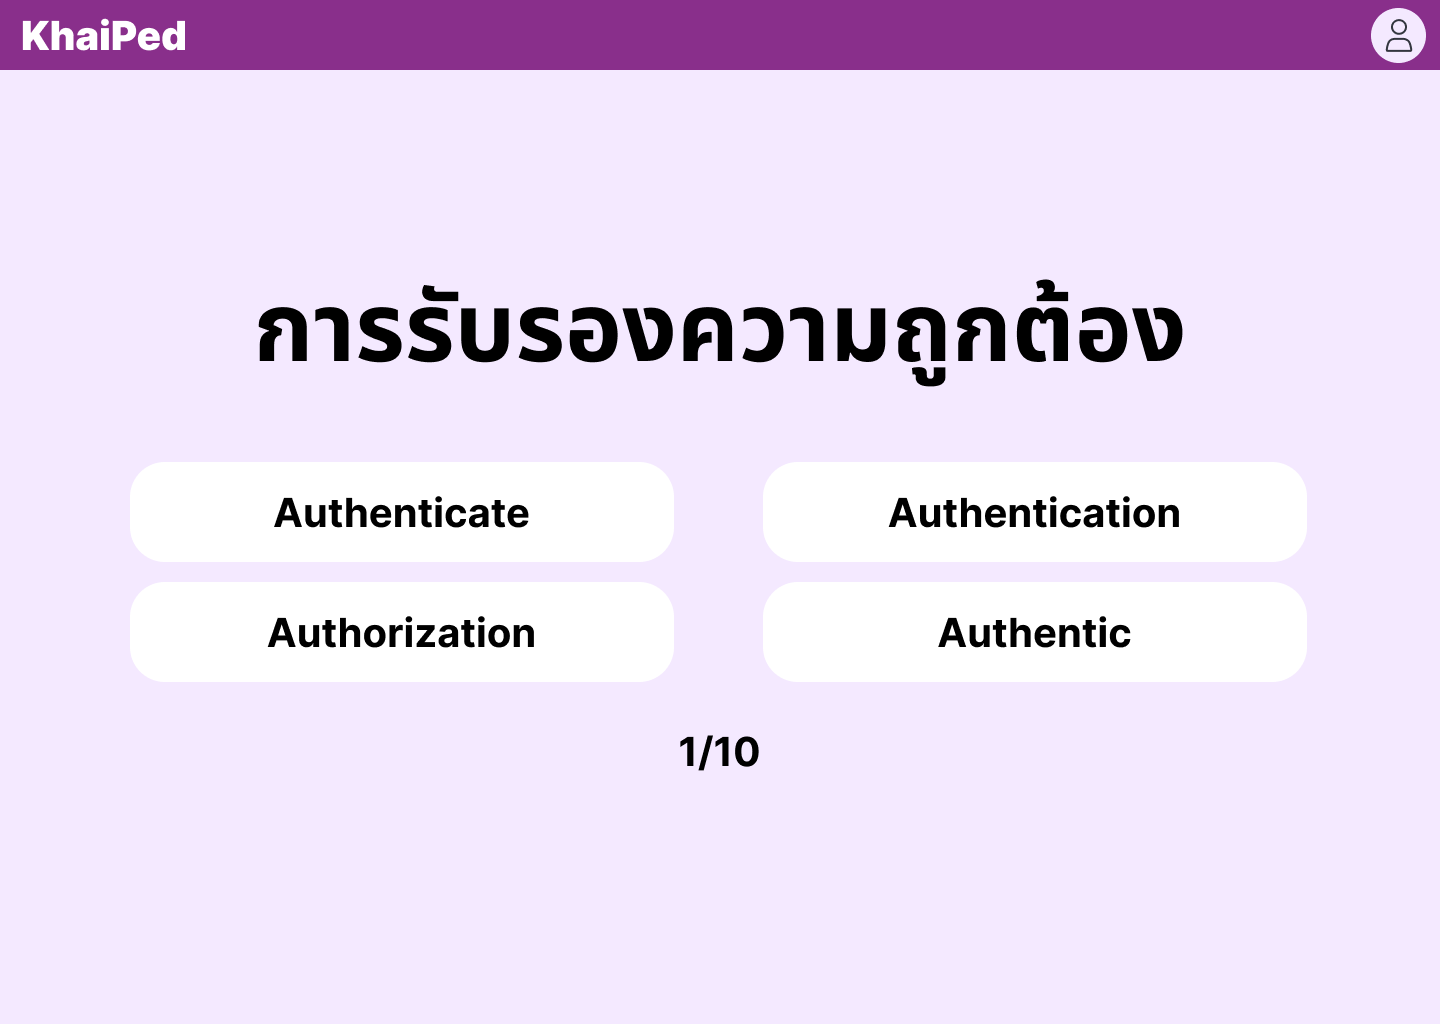
\includegraphics[width=0.8\textwidth, keepaspectratio=true]{image/chap3/ui/quiz/Quiz - Start.png}
	\caption{หน้าเริ่มการทำแบบทดสอบ}\label{fig:UI_QuizStart}
\end{figure}
\hspace{1cm}
จากรูปภาพที่ \ref{fig:UI_Quiz} เมื่อผู้ใช้กดปุ่มเริ่มทำแบบทดสอบแล้ว ระบบจะแสดงผลหน้าสำหรับทำแบบทดสอบ โดยจะประกอบไปด้วยโจทย์
ตัวเลือก 4 ข้อ และจำนวนข้อที่เหลืออยู่ ซึ่งแสดงให้เห็นดังรูปภาพที่ \ref{fig:UI_QuizStart}

\begin{figure}[!h]\centering
	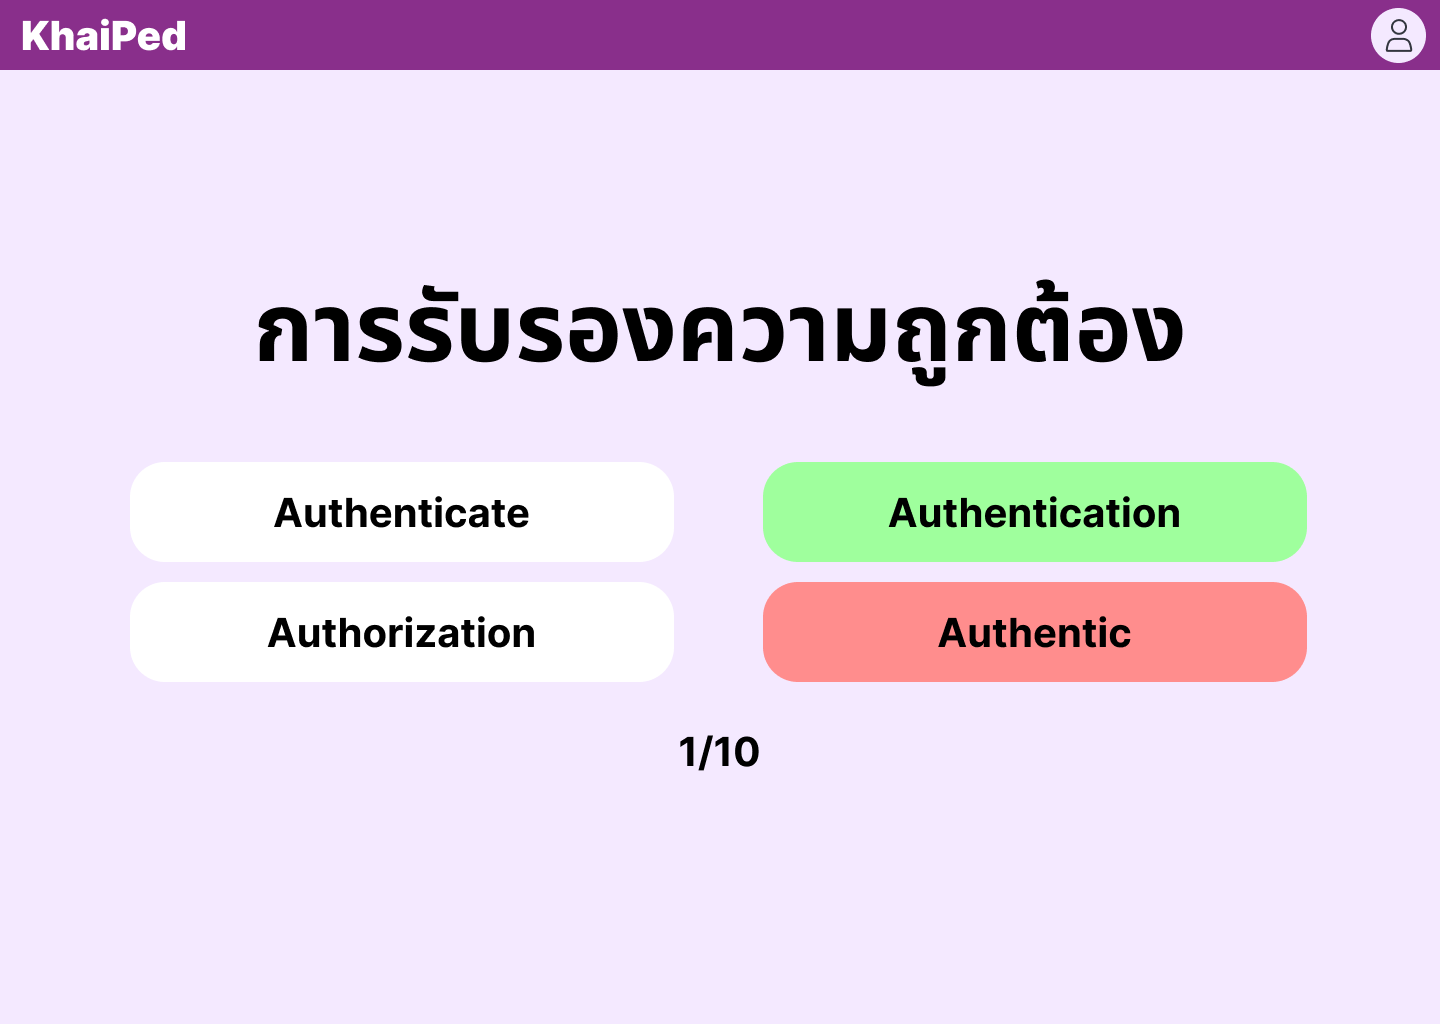
\includegraphics[width=0.8\textwidth, keepaspectratio=true]{image/chap3/ui/quiz/Quiz - Wrong Answer.png}
	\caption{การแสดงผลหากตอบผิด}\label{fig:UI_QuizWrong}
\end{figure}
\hspace{1cm}
หากผู้ใช้เลือกคำตอบผิด ระบบจะแสดงว่าคำตอบที่เลือกผิดโดยขึ้นเป็นสีแดง แล้วแสดงคำตอบที่ถูกเป็นสีเขียว จากนั้นจะแสดงผลข้อถัดไป ดังรูปภาพที่ \ref{fig:UI_QuizWrong}

\pagebreak
\begin{figure}[!h]\centering
	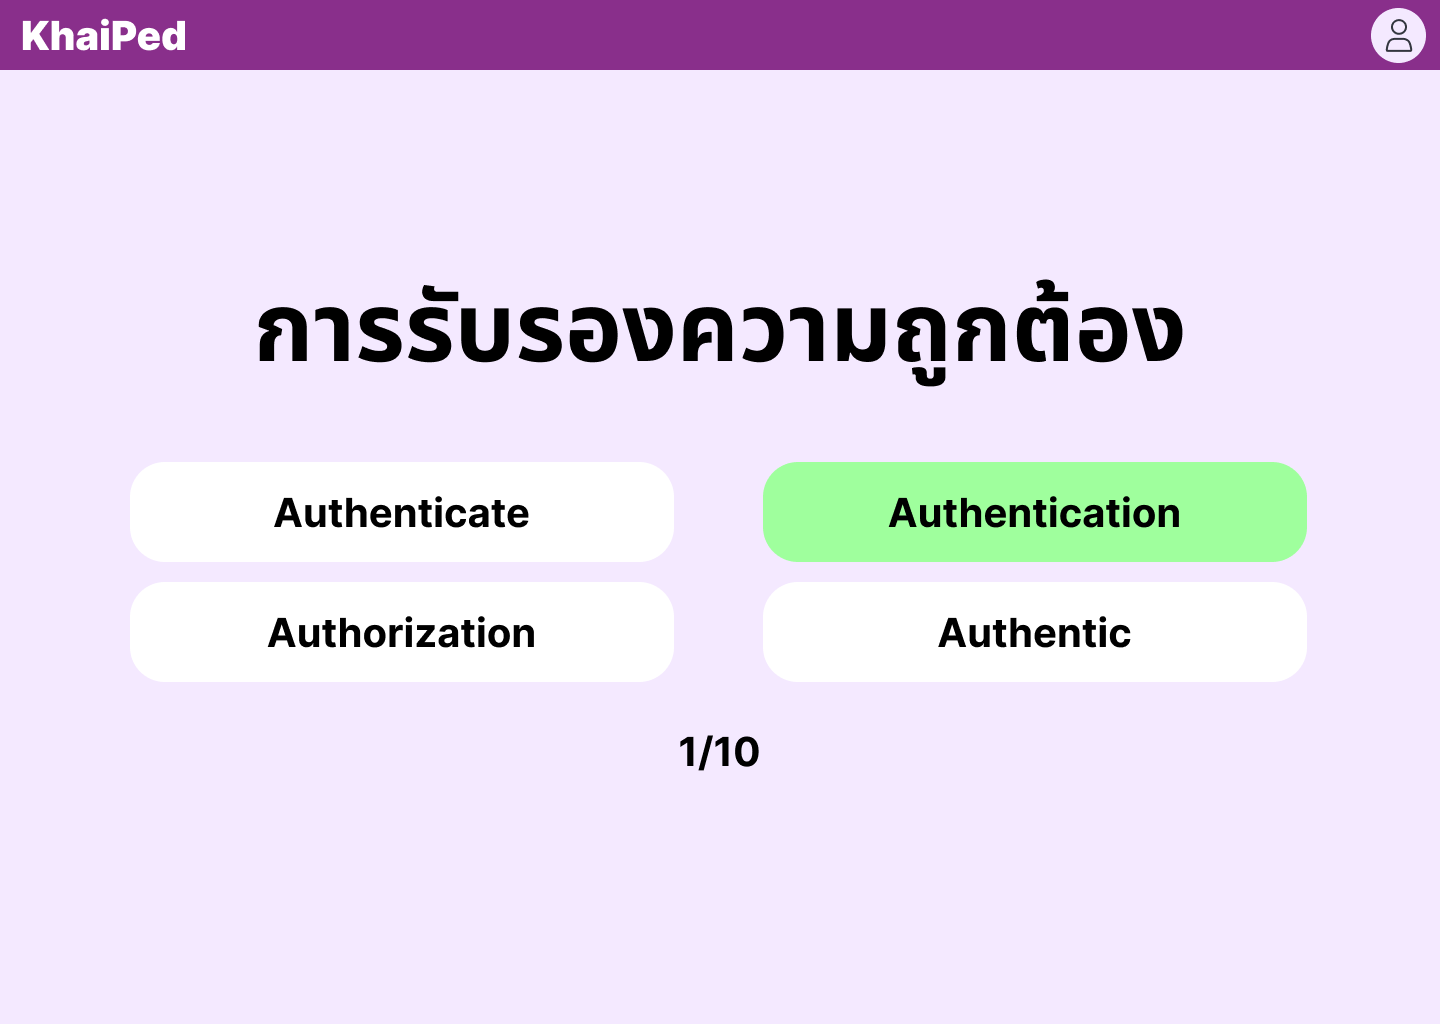
\includegraphics[width=0.8\textwidth, keepaspectratio=true]{image/chap3/ui/quiz/Quiz - Correct Answer.png}
	\caption{การแสดงผลหากตอบถูก}\label{fig:UI_QuizCorrect}
\end{figure}
\hspace{1cm}
หากผู้ใช้เลือกคำตอบถูก ระบบจะแสดงว่าคำตอบที่เลือกถูกเป็นสีเขียว จากนั้นจะแสดงผลข้อถัดไป ดังรูปภาพที่ \ref{fig:UI_QuizCorrect}

\begin{figure}[!h]\centering
	\includegraphics[width=0.8\textwidth, keepaspectratio=true]{image/chap3/ui/quiz/Quiz - Result.png}
	\caption{การแสดงผลลัพท์การทำแบบทดสอบ}\label{fig:UI_QuizResult}
\end{figure}
\hspace{1cm}
หากผู้ใช้ตอบคำถามครบ 10 ข้อแล้ว ระบบจะแสดงคำตอบของข้อนั้น ๆ แล้วแจ้งเตือนคะแนนที่ผู้ใช้ทำได้ ผู้ใช้สามารถกดปุ่มออกเพื่อกลับไปหน้าหลักได้ ดังรูปภาพที่ \ref{fig:UI_QuizResult}
หรือกดปุ่มทำแบบทดสอบใหม่ เพื่อให้ระบบจะสุ่มคำศัพท์มาทำแบบทดสอบใหม่ได้

\pagebreak
\subsection{พจนานุกรม}
\begin{figure}[!h]\centering
	\includegraphics[width=0.8\textwidth, keepaspectratio=true]{image/chap3/ui/dict/Dictionary.png}
	\caption{หน้าหลักของพจนานุกรม}\label{fig:UI_Dictionary}
\end{figure}
\hspace{1cm}
จากรูปภาพที่ \ref{fig:UI_Home} เมื่อผู้ใช้กดปุ่มพจนานุกรม ระบบจะแสดงผลหน้าหลักของพจนานุกรม ซึ่งแสดงให้เห็นดังรูปภาพที่ \ref{fig:UI_Dictionary}
โดยในหน้าจะประกอบไปด้วยช่องค้นหา (1) เมื่อค้นหาแล้ว ระบบจะทำการค้นหาคำศัพท์ในฐานข้อมูลแล้วทำการแสดงผล

\begin{figure}[!h]\centering
	\includegraphics[width=0.8\textwidth, keepaspectratio=true]{image/chap3/ui/dict/Dictionary - Search Word.png}
	\caption{หน้าแสดงผลการค้นหา}\label{fig:UI_DictionarySearch}
\end{figure}
\hspace{1cm}
เมื่อผู้ใช้ค้นหาคำศัพท์จากช่องค้นหา หรือในหน้าพจนานุกรม ระบบจะแสดงผลการ์ดคำศัพท์ที่ทำการค้นหาออกมา
ดังรูปภาพที่ \ref{fig:UI_DictionarySearch} โดยจะสามารถกดปุ่มดูรายละเอียด (1) เพื่อดูรายละเอียดคำศัพท์นั้น ๆ ได้

\pagebreak
\begin{figure}[!h]\centering
	\includegraphics[width=0.8\textwidth, keepaspectratio=true]{image/chap3/ui/dict/Dictionary - View Word.png}
	\caption{การแสดงผลรายละเอียดคำศัพท์}\label{fig:UI_DictionaryView}
\end{figure}
\hspace{1cm}
จากรูปภาพที่ \ref{fig:UI_DictionarySearch} เมื่อผู้ใช้กดปุ่มแสดงรายละเอียด ระบบจะแสดงผลรายละเอียดของคำนั้น ๆ ดังรูปภาพที่ \ref{fig:UI_DictionaryView}
โดยสามารถกดปุ่มปิด หรือกดปุ่มเล่นเสียงที่เล่นเสียงวิธีการออกเสียงของคำศัพท์ได้

\pagebreak
\section{Database Design}
\subsection{Entity-Relationship Diagram} \label{ssec:DB}
\begin{figure}[!h]\centering
	\includegraphics[width=\textwidth, keepaspectratio=true]{image/chap3/ER diagrams.jpg}
	\caption{แบบจำลองโครงสร้างของฐานข้อมูล}\label{fig:ERDiagram}
\end{figure}
\hspace{1cm}
จากรูปภาพที่ \ref{fig:ERDiagram} ฐานข้อมูลจะประกอบไปด้วย 4 ตาราง โดย Word จะมีไว้สำหรับเก็บข้อมูลของคำศัพท์ Word Root
จะเก็บรากของคำศัพท์ User จะเก็บข้อมูลต่าง ๆ ของผู้ใช้ และ Word Learned จะเก็บคำศัพท์ที่ผู้ใช้ได้เคยเรียนรู้ไปแล้ว

\pagebreak
\subsection{Data Dictionary}
\subsubsection{Word}
\hspace{1cm}
ตารางที่ \ref{tbl:Word} มีไว้สำหรับเก็บข้อมูลต่าง ๆ ของคำศัพท์
\begin{table}[h]\centering
	\caption{ตาราง Word}\label{tbl:Word}
	\begin{tabular}[t]{|p{.02\linewidth}|p{.15\linewidth}|p{.15\linewidth}|p{.025\linewidth}|p{.25\linewidth}|p{.25\linewidth}|}
		\hline
		\multicolumn{1}{|c|}{Key} & \multicolumn{1}{c|}{Attribute} & \multicolumn{1}{c|}{Domain}                                                                                                                   & \multicolumn{1}{c|}{Null} & \multicolumn{1}{c|}{Description}                                                                     & \multicolumn{1}{c|}{Example}                                                                                                    \\ \hline
		PK                        & id                             & int                                                                                                                                           & No                        & \begin{tabular}[c]{@{}l@{}}เลขสำหรับระบุคำศัพท์\\ เป็นตัวเลขที่ต่อเนื่องกันไปไม่ซ้ำ\\ \end{tabular}                   & 1                                                                                                                               \\ \hline
		\textbf{}                 & word                           & varchar(64)                                                                                                                                   & No                        & คำศัพท์ภาษาอังกฤษ                                                                                        & Authentication                                                                                                                  \\ \hline
		\textbf{}                 & tran\_th                       & text                                                                                                                                          & No                        & ความหมายภาษาไทย                                                                                      & การรับรองความถูกต้อง                                                                                                               \\ \hline
		\textbf{}                 & tran\_eng                      & text                                                                                                                                          & No                        & ความหมายภาษาอังกฤษ                                                                                    & \begin{tabular}[c]{@{}l@{}}the act of proving that \\ something is real, true or \\ what somebody claims it is \\ \end{tabular} \\ \hline
		FK                        & root\_id                       & int                                                                                                                                           & No                        & \begin{tabular}[c]{@{}l@{}}เลขสำหรับระบุรากของคำศัพท์\\ เป็นตัวเลขที่ต่อเนื่องกันไปไม่ซ้ำ\\ \end{tabular}             & 1                                                                                                                               \\ \hline
		\textbf{}                 & part\_of\_speech               & \begin{tabular}[c]{@{}l@{}}enum\\ (noun,\\ pronoun,\\ verb,\\ adjective,\\ adverb,\\	preposition,\\	conjunction,\\ interjection)\end{tabular} & No                        & \begin{tabular}[c]{@{}l@{}}ประเภทของคำในภาษาอังกฤษ\\ แบ่งตามหน้าที่ \\ โดยแบ่งได้ทั้งหมด 8 ประเภท\end{tabular} & noun                                                                                                                            \\ \hline
		FK                        & synonyms                       & int                                                                                                                                           & Yes                       & \begin{tabular}[c]{@{}l@{}}เลขสำหรับระบุคำพ้องความหมาย \\ เป็นตัวเลขที่ต่อเนื่องกันไปไม่ซ้ำ  \\ \end{tabular}        & 2                                                                                                                               \\ \hline
	\end{tabular}
\end{table}

\subsubsection{Word Root}
\hspace{1cm}
ตารางที่ \ref{tbl:WordRoot} มีไว้สำหรับเก็บข้อมูลรากของคำศัพท์
\begin{table}[h]\centering
	\caption{ตาราง Word Root}\label{tbl:WordRoot}
	\begin{tabular}[t]{|p{.02\linewidth}|p{.15\linewidth}|p{.15\linewidth}|p{.025\linewidth}|p{.25\linewidth}|p{.25\linewidth}|}
		\hline
		\multicolumn{1}{|c|}{Key} & \multicolumn{1}{c|}{Attribute} & \multicolumn{1}{c|}{Domain} & \multicolumn{1}{c|}{Null} & \multicolumn{1}{c|}{Description}                                                         & \multicolumn{1}{c|}{Example} \\ \hline
		PK                        & id                             & int                         & No                        & \begin{tabular}[c]{@{}l@{}}เลขสำหรับระบุรากของคำศัพท์\\ เป็นตัวเลขที่ต่อเนื่องกันไปไม่ซ้ำ\\ \end{tabular} & 1                            \\ \hline
		\textbf{}                 & root                           & varchar(64)                 & No                        & รากของคำศัพท์                                                                               & authentic                    \\ \hline
		\textbf{}                 & pic                            & text                        & Yes                       & ลิงคที่เก็บรูปของรากคำศัพท์                                                                      & root/1                       \\ \hline
	\end{tabular}
\end{table}

\pagebreak
\subsubsection{User}
\hspace{1cm}
ตารางที่ \ref{tbl:User} มีไว้สำหรับเก็บข้อมูลต่าง ๆ ของผู้ใช้
\begin{table}[h]\centering
	\caption{ตาราง User}\label{tbl:User}
	\begin{tabular}[t]{|p{.02\linewidth}|p{.15\linewidth}|p{.15\linewidth}|p{.025\linewidth}|p{.25\linewidth}|p{.25\linewidth}|}
		\hline
		\multicolumn{1}{|c|}{Key} & \multicolumn{1}{c|}{Attribute} & \multicolumn{1}{c|}{Domain} & \multicolumn{1}{c|}{Null} & \multicolumn{1}{c|}{Description}                                                  & \multicolumn{1}{c|}{Example} \\ \hline
		PK                        & id                             & int                         & No                        & \begin{tabular}[c]{@{}l@{}}เลขสำหรับระบุผู้ใช้\\ เป็นตัวเลขที่ต่อเนื่องกันไปไม่ซ้ำ\\ \end{tabular} & 1                            \\ \hline
		\textbf{}                 & username                       & varchar(32)                 & No                        & ชื่อผู้ใช้สำหรับการเข้าสู่ระบบ                                                              & khaiped                      \\ \hline
		\textbf{}                 & password                       & varchar(32)                 & No                        & รหัสผ่านสำหรับการเข้าสู่ระบบ                                                             & Khaiped@01                   \\ \hline
		\textbf{}                 & game\_played                   & int                         & No                        & จำนวนเกมที่เคยเล่น                                                                    & 15                           \\ \hline
		\textbf{}                 & quiz\_score                    & int                         & No                        & คะแนนของแบบทดสอบที่เคยทำ                                                             & 87                           \\ \hline
		\textbf{}                 & quiz\_taken                    & int                         & No                        & จำนวนแบบทดสอบที่เคยทำ                                                                 & 10                           \\ \hline
		\textbf{}                 & day\_streak                    & int                         & No                        & \begin{tabular}[c]{@{}l@{}}จำนวนวันที่เข้าใช้งาน \\ แอปพลิเคชันติดกันสูงสุด  \\ \end{tabular} & 16                           \\ \hline
		\textbf{}                 & last\_login                    & date                        & No                        & เวลาที่เข้าสู่ระบบล่าสุด                                                                 & 2023-06-05 16:13:23          \\ \hline
		\textbf{}                 & score                          & int                         & No                        & คะแนนที่ได้                                                                          & 200                          \\ \hline
	\end{tabular}
\end{table}

\subsubsection{Word Learned}
\hspace{1cm}
ตารางที่ \ref{tbl:WordLearned} มีไว้สำหรับเก็บข้อมูลคำศัพท์ที่ผู้ใช้เคยเรียนไปแล้ว
\begin{table}[h]\centering
	\caption{ตาราง Word Learned}\label{tbl:WordLearned}
	\begin{tabular}[t]{|p{.02\linewidth}|p{.15\linewidth}|p{.15\linewidth}|p{.025\linewidth}|p{.25\linewidth}|p{.25\linewidth}|}
		\hline
		\multicolumn{1}{|c|}{Key} & \multicolumn{1}{c|}{Attribute} & \multicolumn{1}{c|}{Domain} & \multicolumn{1}{c|}{Null} & \multicolumn{1}{c|}{Description}                                                            & \multicolumn{1}{c|}{Example} \\ \hline
		PK                        & id                             & int                         & No                        & \begin{tabular}[c]{@{}l@{}}เลขสำหรับระบุคำศัพท์ที่เคยเรียน \\ เป็นตัวเลขที่ต่อเนื่องกันไปไม่ซ้ำ\\ \end{tabular} & 1                            \\ \hline
		FK                        & user\_id                       & int                         & No                        & \begin{tabular}[c]{@{}l@{}}เลขสำหรับระบุคำศัพท์\\ เป็นตัวเลขที่ต่อเนื่องกันไปไม่ซ้ำ\\ \end{tabular}          & 1                            \\ \hline
		FK                        & word\_id                       & int                         & No                        & \begin{tabular}[c]{@{}l@{}}เลขสำหรับระบุผู้ใช้\\ เป็นตัวเลขที่ต่อเนื่องกันไปไม่ซ้ำ\\ \end{tabular}           & 1                            \\ \hline
	\end{tabular}
\end{table}

%%%%%%%%%%%%%%%%%%%%%%%%%%%%%%%%%%%%%%%%%%%%%%%%%%%%%%%%%%%%%%%
%%%%%%%%%%%%%%%%%%%%%%%%%% Chapter 4 %%%%%%%%%%%%%%%%%%%%%%%%%%
%%%%%%%%%%%%%%%%%%%%%%%%%%%%%%%%%%%%%%%%%%%%%%%%%%%%%%%%%%%%%%%

\chapter{ผลการดำเนินงานและอภิปรายผล}

\hspace{1cm}
ผู้จัดทำได้นำการออกแบบ User Interface ในหัวข้อที่ \ref{ssec:UI} และ Database ในหัวข้อที่ \ref{ssec:DB}
มาเป็นข้อมูลอ้างอิงในการพัฒนาตัวเว็บแอปพลิเคชัน โดยการออกแบบจะอ้างอิงจากผลของแบบสอบถามที่ได้สอบถามผู้ที่มีความสนใจในการสอบ TOEIC 
ซึ่งจะแสดงผลการดำเนินการได้ดังต่อไปนี้

\section{ฐานข้อมูล}
\hspace{1cm}
ผู้จัดทำได้ทำการพัฒนาในส่วนของ Backend ด้วยการใช้ Django และได้ทำการสร้าง Database ตามการออกแบบในหัวข้อที่ \ref{ssec:DB}
ดังนี้

\begin{figure}[!h]\centering
	\includegraphics[width=\textwidth, keepaspectratio=true]{image/chap4/DB/db.png}
	\caption{{ฐานข้อมูลที่พัฒนาขึ้น}}\label{fig:chap4DB}
\end{figure}
\hspace{1cm}
จากรูปภาพที่ \ref{fig:chap4DB} จะเห็นว่า ฐานข้อมูลจะประกอบไปด้วย 4 ตารางตามที่ได้ออกแบบไว้คือ User, Word Learned,
Word Root และ Word

\pagebreak
\begin{figure}[!h]\centering
	\includegraphics[width=\textwidth, keepaspectratio=true]{image/chap4/DB/user.png}
	\caption{{ฐานข้อมูลสำหรับ User}}\label{fig:chap4User}
\end{figure}
\hspace{1cm}
จากรูปภาพที่ \ref{fig:chap4User} จะเห็นว่า ฐานข้อมูลของ User ที่ใช้สำหรับเก็บข้อมูลของผู้ใช้
จะประกอบไปด้วย Username สำหรับเก็บชื่อผู้ใช้สำหรับการเข้าสู่ระบบ
Password สำหรับเก็บรหัสผ่านสำหรับการเข้าสู่ระบบ Game Played เก็บ จํานวนเกมที่เคยเล่น
Quiz Score เก็บคะแนนของแบบทดสอบที่เคยทํา Quiz Taken เก็บจํานวนแบบทดสอบที่เคยทํา
Day Streak เก็บจํานวนวันที่เข้าใช้งานแอปพลิเคชันติดกันสูงสุด และ Last Login เก็บเวลาที่เข้าสู่ระบบล่าสุด

\begin{figure}[!h]\centering
	\includegraphics[width=\textwidth, keepaspectratio=true]{image/chap4/DB/word learned.png}
	\caption{{ฐานข้อมูลสำหรับ Word Learned}}\label{fig:chap4WordLearned}
\end{figure}
\hspace{1cm}
จากรูปภาพที่ \ref{fig:chap4WordLearned} จะเห็นว่า ฐานข้อมูลของ Word Learned จะมีไว้สำหรับเก็บข้อมูลคำศัพท์ที่ผู้ใช้เคยเรียนไปแล้ว
ซึ่งประกอบไปด้วย User id สำหรับระบุผู้ใช้ และ Word id สำหรับระบุคำศัพท์

\pagebreak
\begin{figure}[!h]\centering
	\includegraphics[width=\textwidth, keepaspectratio=true]{image/chap4/DB/word root.png}
	\caption{{ฐานข้อมูลสำหรับ Word Root}}\label{fig:chap4WordRoot}
\end{figure}
\hspace{1cm}
จากรูปภาพที่ \ref{fig:chap4WordRoot} จะเห็นว่า ฐานข้อมูลของ Word Root จะมีไว้สำหรับเก็บข้อมูลรากของคำศัพท์
ซึ่งประกอบไปด้วย Root สำหรับเก็บรากของคำศัพท์และ Pic สำหรับรูปภาพที่ระบุถึงรากของคำศัพท์

\begin{figure}[!h]\centering
	\includegraphics[width=\textwidth, keepaspectratio=true]{image/chap4/DB/word.png}
	\caption{{ฐานข้อมูลสำหรับ Word}}\label{fig:chap4Word}
\end{figure}
\hspace{1cm}
และสุดท้าย รูปภาพที่ \ref{fig:chap4WordRoot} จะเห็นว่า ฐานข้อมูลของ Word จะมีไว้สำหรับเก็บข้อมูลของคำศัพท์
ซึ่งประกอบไปด้วย Word สำหรับเก็บคำศัพท์ Tran th สำหรับเก็บความหมายภาษาไทย Tran eng สำหรับเก็บความหมายภาษาอังกฤษ
Root id สำหรับเก็บรากของคำศัพท์นั้น ๆ  Synonyms สำหรับเก็บคำที่พ้องความหมายและ Part of speech 

\pagebreak
\section{การพัฒนาเว็บแอปพลิเคชันฝั่งผู้ใช้รุ่นต้นแบบ}
\hspace{1cm}
ผู้จัดทำได้ทำการพัฒนาในส่วนของ Frontend ด้วยการใช้ React ควบคู่กับ Tailwind CSS และได้ทำการสร้าง User Interface
ตามการออกแบบในหัวข้อที่ \ref{ssec:UI} ดังนี้

\begin{figure}[!h]\centering
	\includegraphics[width=\textwidth, keepaspectratio=true]{image/chap4/UI/home/home.png}
	\caption{{หน้าหลัก}}\label{fig:chap4UIHome}
\end{figure}
\hspace{1cm}
หน้าหลักของแอปพลิเคชัน ซึ่งได้พัฒนาตามการออกแบบในรูปภาพที่ \ref{fig:UI_Home} และได้ผลดังที่เห็นในภาพที่ \ref{fig:chap4UIHome}

\begin{figure}[!h]\centering
	\includegraphics[width=\textwidth, keepaspectratio=true]{image/chap4/UI/home/home help.png}
	\caption{{กดปุ่มช่วยเหลือ}}\label{fig:chap4UIHomeHelp}
\end{figure}
\hspace{1cm}
เมื่อกดปุ่มช่วยเหลือ จะแสดงกล่องข้อความพร้อมวิธีใช้ดังที่เห็นในภาพที่ \ref{fig:chap4UIHomeHelp}

\pagebreak
\begin{figure}[!h]\centering
	\includegraphics[width=\textwidth, keepaspectratio=true]{image/chap4/UI/home/guest button.png}
	\caption{{ปุ่มผู้ใช้หากไม่ได้เข้าสู่ระบบ}}\label{fig:chap4UIGuestButton}
\end{figure}
\hspace{1cm}
ปุ่มผู้ใช้หากไม่ได้เข้าสู่ระบบ เมื่อกดแล้วจะแสดงปุ่มลงทะเบียน และปุ่มเข้าสู่ระบบ ได้ผลดังที่เห็นในภาพที่ \ref{fig:chap4UIGuestButton}

\begin{figure}[!h]\centering
	\includegraphics[width=\textwidth, keepaspectratio=true]{image/chap4/UI/login/login.png}
	\caption{{หน้าเข้าสู่ระบบ}}\label{fig:chap4UILogIn}
\end{figure}
\hspace{1cm}
เมื่อกดปุ่มเข้าสู่ระบบแล้ว จะแสดงผลหน้าเข้าสู่ระบบ ซึ่งแตกต่างจากการออกแบบที่เห็นในรูปภาพที่ \ref{fig:UI_LoginPage}
โดยจะแยกหน้าเข้าสู่ระบบและหน้าลงทะเบียนผู้ใช้แยกออกจากกัน และจะมีปุ่มที่พาไปยังหน้าลงทะเบียน ดังที่เห็นในภาพที่ \ref{fig:chap4UILogIn}

\pagebreak
\begin{figure}[!h]\centering
	\includegraphics[width=\textwidth, keepaspectratio=true]{image/chap4/UI/login/register.png}
	\caption{{หน้าลงทะเบียน}}\label{fig:chap4UIRegister}
\end{figure}
\hspace{1cm}
เมื่อกดปุ่มลงทะเบียน จะแสดงผลหน้าลงทะเบียน ดังที่เห็นในภาพที่ \ref{fig:chap4UIRegister}

\begin{figure}[!h]\centering
	\includegraphics[width=\textwidth, keepaspectratio=true]{image/chap4/UI/login/register success.png}
	\caption{{การลงทะเบียนผู้ใช้งานสำเร็จ}}\label{fig:chap4UIRegisterSuccess}
\end{figure}
\hspace{1cm}
เมื่อเข้าสู่หน้าลงทะเบียน และกรอกข้อมูลผู้ใช้ จากนั้นกดปุ่มลงทะเบียน หากข้อมูลที่กรอกถูกต้อง ระบบจะแสดงผลว่าลงทะเบียนสำเร็จ
ดังที่เห็นในภาพที่ \ref{fig:chap4UIRegisterSuccess} และแสดงผลหน้าเข้าสู่ระบบ

\pagebreak
\begin{figure}[!h]\centering
	\includegraphics[width=\textwidth, keepaspectratio=true]{image/chap4/UI/login/register failed.png}
	\caption{{การลงทะเบียนผู้ใช้งานไม่สำเร็จ}}\label{fig:chap4UIRegisterFailed}
\end{figure}
\hspace{1cm}
หากกรอกข้อมูลผู้ใช้ที่ซ้ำกับในระบบ จะแสดงผลว่าชื่อผู้ใช้ได้ถูกใช้ไปแล้ว ดังที่เห็นในภาพที่ \ref{fig:chap4UIRegisterFailed}

\begin{figure}[!h]\centering
	\includegraphics[width=\textwidth, keepaspectratio=true]{image/chap4/UI/login/login success.png}
	\caption{{การเข้าสู่ระบบสำเร็จ}}\label{fig:chap4UILogInSuccess}
\end{figure}
\hspace{1cm}
เมื่อเข้าสู่หน้าเข้าสู่ระบบ และกรอกข้อมูลผู้ใช้ จากนั้นกดปุ่มเข้าสู่ระบบ หากข้อมูลที่กรอกถูกต้อง ระบบจะแสดงผลว่าเข้าสู่ระบบสำเร็จ
ดังที่เห็นในภาพที่ \ref{fig:chap4UILogInSuccess} และแสดงผลหน้าหลัก

\pagebreak
\begin{figure}[!h]\centering
	\includegraphics[width=\textwidth, keepaspectratio=true]{image/chap4/UI/login/login failed.png}
	\caption{{การเข้าสู่ระบบไม่สำเร็จ}}\label{fig:chap4UILogInFailed}
\end{figure}
\hspace{1cm}
หากกรอกข้อมูลผู้ใช้ที่ไม่ถูกต้อง จะแสดงผลว่าชื่อผู้ใช้หรือรหัสผ่านไม่ถูกต้อง ดังที่เห็นในภาพที่ \ref{fig:chap4UILogInFailed}


\begin{figure}[!h]\centering
	\includegraphics[width=\textwidth, keepaspectratio=true]{image/chap4/UI/stat/user button.png}
	\caption{{ปุ่มผู้ใช้หากเข้าสู่ระบบสำเร็จ}}\label{fig:chap4UIUserButton}
\end{figure}
\hspace{1cm}
เมื่อเข้าสู่หน้าเข้าสู่ระบบสำเร็จ หากกดปุ่มผู้ใช้ จะแสดงผลปุ่มเพื่อพาไปหน้าสถิติ ปุ่มเพื่อพาไปหน้ากระดานผู้นำ และปุ่มออกจากระบบ 
ซึ่งสามารถกดเพื่อออกจากระบบ ดังที่เห็นในภาพที่ \ref{fig:chap4UIUserButton}

\pagebreak
\begin{figure}[!h]\centering
	\includegraphics[width=\textwidth, keepaspectratio=true]{image/chap4/UI/stat/stat.png}
	\caption{{หน้าสถิติการใช้งานเว็บแอปพลิเคชัน}}\label{fig:chap4UIStat}
\end{figure}
\hspace{1cm}
เมื่อกดปุ่มหน้าสถิติ ระบบจะทำการแสดงผลหน้าสถิติ ดังที่เห็นในภาพที่ \ref{fig:chap4UIStat}
โดยผู้ใช้สามารถกดปุ่มลูกตา เพื่อดูรายการคำศัพท์ที่เคยเรียนไปแล้วได้

\begin{figure}[!h]\centering
	\includegraphics[width=\textwidth, keepaspectratio=true]{image/chap4/UI/stat/word learned.png}
	\caption{{หน้าคำศัพท์ที่ผู้ใช้ได้เคยเรียนรู้}}\label{fig:chap4UIStatWord}
\end{figure}
\hspace{1cm}
เมื่อกดปุ่มคำศัพท์ที่ผู้ใช้ได้เคยเรียนรู้ ระบบจะทำการแสดงรายการของคำศัพท์ที่ผู้ใช้ได้เรียนรู้ผ่านการใช้งานบัตรคำ
และสามารถกดปุ่มลูกตาเพื่อดูรายละเอียดของคำศัพท์นั้น ๆ ได้ ดังที่เห็นในภาพที่ \ref{fig:chap4UIStatWord}

\pagebreak
\begin{figure}[!h]\centering
	\includegraphics[width=\textwidth, keepaspectratio=true]{image/chap4/UI/stat/word detail.png}
	\caption{{รายละเอียดของคำศัพท์}}\label{fig:chap4UIStatWordDetail}
\end{figure}
\hspace{1cm}
เมื่อกดปุ่มดูรายละเอียดคำศัพท์ ระบบจะทำการแสดงรายรายละเอียดของคำศัพท์นั้น ๆ
ดังที่เห็นในภาพที่ \ref{fig:chap4UIStatWordDetail}

\begin{figure}[!h]\centering
	\includegraphics[width=\textwidth, keepaspectratio=true]{image/chap4/UI/stat/leaderboard.png}
	\caption{{หน้าสถิติการใช้งานเว็บแอปพลิเคชัน}}\label{fig:chap4UILead}
\end{figure}
\hspace{1cm}
เมื่อกดปุ่มหน้ากระดานผู้นำ ระบบจะทำการแสดงผลหน้ากระดานผู้นำ ดังที่เห็นในภาพที่ \ref{fig:chap4UILead}

\pagebreak
\begin{figure}[!h]\centering
	\includegraphics[width=\textwidth, keepaspectratio=true]{image/chap4/UI/random.png}
	\caption{{การสุ่มคำศัพท์ใหม่เพื่อการเรียนรู้}}\label{fig:chap4UIRandom}
\end{figure}
\hspace{1cm}
เมื่อกดปุ่มสุ่มคำศัพท์ใหม่เพื่อการเรียนรู้ในหน้าหลัก ระบบจะทำการแสดงการ์ดคำศัพท์ ดังที่เห็นในภาพที่ \ref{fig:chap4UIRandom}

\begin{figure}[!h]\centering
	\includegraphics[width=\textwidth, keepaspectratio=true]{image/chap4/UI/flashcard/flashcard.png}
	\caption{{หน้าหลักบัตรคำ}}\label{fig:chap4UIFlash}
\end{figure}
\hspace{1cm}
เมื่อกดปุ่มบัตรคำในหน้าหลัก ระบบจะทำการแสดงหน้าหลักบัตรคำ ที่ประกอบไปด้วยปุ่มเริ่ม และปุ่มช่วยเหลือ
ดังที่เห็นในภาพที่ \ref{fig:chap4UIFlash}

\pagebreak
\begin{figure}[!h]\centering
	\includegraphics[width=\textwidth, keepaspectratio=true]{image/chap4/UI/flashcard/flashcard help.png}
	\caption{{กดปุ่มช่วยเหลือหน้าบัตรคำ}}\label{fig:chap4UIFlashHelp}
\end{figure}
\hspace{1cm}
เมื่อกดปุ่มช่วยเหลือในหน้าบัตรคำ จะแสดงกล่องข้อความพร้อมวิธีใช้บัตรคำ ดังที่เห็นในภาพที่ \ref{fig:chap4UIFlashHelp}

\begin{figure}[!h]\centering
	\includegraphics[width=\textwidth, keepaspectratio=true]{image/chap4/UI/flashcard/front.png}
	\caption{{ด้านหน้าของบัตรคำ}}\label{fig:chap4UIFlashFront}
\end{figure}
\hspace{1cm}
เมื่อกดปุ่มเริ่มใช้งานบัตรคำ ระบบจะทำการแสดงบัตรคำด้านหน้า โดยจะมีปุ่มที่กดเมื่อจำศัพท์ได้ กับปุ่มที่กดเมื่อจำศัพท์ไม่ได้
ดังที่เห็นในภาพที่ \ref{fig:chap4UIFlashFront}

\pagebreak
\begin{figure}[!h]\centering
	\includegraphics[width=\textwidth, keepaspectratio=true]{image/chap4/UI/flashcard/back.png}
	\caption{{ด้านหลังของบัตรคำ}}\label{fig:chap4UIFlashBack}
\end{figure}
\hspace{1cm}
เมื่อกดที่บัตรคำ ระบบจะแสดงผลด้านหลังบัตรคำ ดังที่เห็นในภาพที่ \ref{fig:chap4UIFlashBack}

\begin{figure}[!h]\centering
	\includegraphics[width=\textwidth, keepaspectratio=true]{image/chap4/UI/flashcard/result.png}
	\caption{{ผลลัพธ์การใช้งานบัตรคำ}}\label{fig:chap4UIFlashResult}
\end{figure}
\hspace{1cm}
เมื่อผู้ใช้กดปุ่มจำศัพท์จนครบทุกคำแล้ว ระบบจะแสดงผลกล่องผลลัพธ์ ซึ่งสามารถกดปุ่มใช้บัตรคำอีกรอบ หรือกดปุ่มออกได้
ดังที่เห็นในภาพที่ \ref{fig:chap4UIFlashResult}

\pagebreak
\begin{figure}[!h]\centering
	\includegraphics[width=\textwidth, keepaspectratio=true]{image/chap4/UI/game/game.png}
	\caption{{หน้าหลักของการเล่นเกมเรียงพยัญชนะเป็นคำศัพท์}}\label{fig:chap4UIGame}
\end{figure}
\hspace{1cm}
เมื่อกดปุ่มเล่นเกมในหน้าหลัก ระบบจะทำการแสดงหน้าหลักการเล่นเกม ที่ประกอบไปด้วยปุ่มเริ่ม และปุ่มช่วยเหลือ
ดังที่เห็นในภาพที่ \ref{fig:chap4UIGame}

\begin{figure}[!h]\centering
	\includegraphics[width=\textwidth, keepaspectratio=true]{image/chap4/UI/game/help.png}
	\caption{{กดปุ่มช่วยเหลือหน้าการเล่นเกม}}\label{fig:chap4UIGameHelp}
\end{figure}
\hspace{1cm}
เมื่อกดปุ่มช่วยเหลือหน้าการเล่นเกม จะแสดงกล่องข้อความพร้อมวิธีเล่นเกม ดังที่เห็นในภาพที่ \ref{fig:chap4UIGameHelp}

\pagebreak
\begin{figure}[!h]\centering
	\includegraphics[width=\textwidth, keepaspectratio=true]{image/chap4/UI/game/start.png}
	\caption{{กดปุ่มเริ่มเล่นเกมเรียงพยัญชนะเป็นคำศัพท์}}\label{fig:chap4UIGameStart}
\end{figure}
\hspace{1cm}
เมื่อกดปุ่มเริ่มเล่นเกม ระบบจะทำการแสดงผลหน้าเล่นเกมที่ประกอบไปด้วย กล่องตัวอักษร คำศัพท์ที่ถูกสลับที่ตัวอักษร
คำใบ้ และช่องสำหรับใส่คำตอบ ดังที่เห็นในภาพที่ \ref{fig:chap4UIGameStart}

\begin{figure}[!h]\centering
	\includegraphics[width=\textwidth, keepaspectratio=true]{image/chap4/UI/game/type.png}
	\caption{{การพิมพ์คำตอบในการเล่นเกม}}\label{fig:chap4UIGameType}
\end{figure}
\hspace{1cm}
เมื่อพิมพ์คำตอบ หากตัวอักษรที่พิมพ์ ตรงกับที่มีในคำศัพท์ ตัวอักษรตัวนั้น ๆ จะเปลี่ยนเป็นสีเทา
ดังที่เห็นในภาพที่ \ref{fig:chap4UIGameType}

\pagebreak
\begin{figure}[!h]\centering
	\includegraphics[width=\textwidth, keepaspectratio=true]{image/chap4/UI/game/wrong.png}
	\caption{{คำที่พิมพ์ในการเล่นเกมไม่ถูกต้อง}}\label{fig:chap4UIGameWrong}
\end{figure}
\hspace{1cm}
หากพิมพ์คำตอบที่ไม่ถูกต้องแล้วกดปุ่มส่ง จะแสดงผลตำแหน่งที่ตัวอักษรถูกเป็นสีเขียว และตำแหน่งที่ผิด
เป็นสีแดง ดังที่เห็นในภาพที่ \ref{fig:chap4UIGameStart}

\begin{figure}[!h]\centering
	\includegraphics[width=\textwidth, keepaspectratio=true]{image/chap4/UI/game/correct.png}
	\caption{{คำที่พิมพ์ในการเล่นเกมถูกต้อง}}\label{fig:chap4UIGameCorrect}
\end{figure}
\hspace{1cm}
หากพิมพ์คำตอบที่ถูกต้องแล้วกดปุ่มส่ง จะแสดงกล่องผลลัพธ์ ซึ่งสามารถกดปุ่มเล่นเกมอีกรอบ หรือกดปุ่มออกได้
ดังที่เห็นในภาพที่ \ref{fig:chap4UIGameCorrect}

\pagebreak
\begin{figure}[!h]\centering
	\includegraphics[width=\textwidth, keepaspectratio=true]{image/chap4/UI/quiz/quiz.png}
	\caption{{หน้าหลักการทำแบบทดสอบ}}\label{fig:chap4UIQuiz}
\end{figure}
\hspace{1cm}
เมื่อกดปุ่มทำแบบทดสอบในหน้าหลัก ระบบจะทำการแสดงหน้าหลักของการทำแบบทดสอบ ที่ประกอบไปด้วยปุ่มเริ่ม และปุ่มช่วยเหลือ
ดังที่เห็นในภาพที่ \ref{fig:chap4UIQuiz}

\begin{figure}[!h]\centering
	\includegraphics[width=\textwidth, keepaspectratio=true]{image/chap4/UI/quiz/help.png}
	\caption{{กดปุ่มช่วยเหลือหน้าทำแบบทดสอบ}}\label{fig:chap4UIQuizHelp}
\end{figure}
\hspace{1cm}
เมื่อกดปุ่มช่วยเหลือหน้าทำแบบทดสอบ จะแสดงกล่องข้อความพร้อมวิธีทำแบบทดสอบ ดังที่เห็นในภาพที่ \ref{fig:chap4UIQuizHelp}

\pagebreak
\begin{figure}[!h]\centering
	\includegraphics[width=\textwidth, keepaspectratio=true]{image/chap4/UI/quiz/start.png}
	\caption{{กดปุ่มเริ่มทำแบบทดสอบ}}\label{fig:chap4UIQuizStart}
\end{figure}
\hspace{1cm}
เมื่อกดปุ่มเริ่มทำแบบทดสอบ ระบบจะทำการแสดงผลหน้าแบบทดสอบที่ประกอบไปด้วย คำถาม และกล่องคำตอบทั้ง 4 ตัวเลือก
ดังที่เห็นในภาพที่ \ref{fig:chap4UIQuizStart}

\begin{figure}[!h]\centering
	\includegraphics[width=\textwidth, keepaspectratio=true]{image/chap4/UI/quiz/wrong.png}
	\caption{{ตอบแบบทดสอบผิด}}\label{fig:chap4UIQuizWrong}
\end{figure}
\hspace{1cm}
เมื่อเลือกคำตอบ หากเลือกคำตอบไม่ถูก กล่องคำตอบที่เลือกจะเปลี่ยนเป็นสีแดง และกล่องคำตอบที่ถูกจะเปลี่ยนเป็นสีเขียว และแสดงผลข้อถัดไป
ดังที่เห็นในภาพที่ \ref{fig:chap4UIQuizWrong}

\pagebreak
\begin{figure}[!h]\centering
	\includegraphics[width=\textwidth, keepaspectratio=true]{image/chap4/UI/quiz/correct.png}
	\caption{{ตอบแบบทดสอบถูก}}\label{fig:chap4UIQuizCorrect}
\end{figure}
\hspace{1cm}
เมื่อเลือกคำตอบ หากเลือกคำตอบถูก กล่องคำตอบที่เลือกจะเปลี่ยนเป็นสีเขียว และแสดงผลข้อถัดไป
ดังที่เห็นในภาพที่ \ref{fig:chap4UIQuizCorrect}

\begin{figure}[!h]\centering
	\includegraphics[width=\textwidth, keepaspectratio=true]{image/chap4/UI/quiz/result.png}
	\caption{{ผลลัพธ์การทำแบบทดสอบ}}\label{fig:chap4UIQuizResult}
\end{figure}
\hspace{1cm}
เมื่อตอบคำถามครบ 10 ข้อแล้ว จะแสดงกล่องผลลัพธ์การทำแบบทดสอบ ซึ่งสามารถกดปุ่มทำแบบทดสอบอีกรอบ หรือกดปุ่มออกได้
ดังที่เห็นในภาพที่ \ref{fig:chap4UIQuizResult}

\pagebreak
\begin{figure}[!h]\centering
	\includegraphics[width=\textwidth, keepaspectratio=true]{image/chap4/UI/dict/dict.png}
	\caption{{หน้าพจนานุกรม}}\label{fig:chap4UIDict}
\end{figure}
\hspace{1cm}
เมื่อกดปุ่มพจนานุกรมในหน้าหลัก ระบบจะทำการแสดงหน้าพจนานุกรม ที่ประกอบไปด้วยช่องสำหรับใส่คำค้นหา
ดังที่เห็นในภาพที่ \ref{fig:chap4UIDict}

\begin{figure}[!h]\centering
	\includegraphics[width=\textwidth, keepaspectratio=true]{image/chap4/UI/dict/result.png}
	\caption{{ผลการค้นหา}}\label{fig:chap4UIDictResult}
\end{figure}
\hspace{1cm}
เมื่อใส่คำค้นหา ทั้งในช่องค้นหน้าในหน้าพจนานุกรม และช่องค้นหน้าบนแถบนำทาง ระบบจะแสดงคำศัพท์ที่ตรงกับคำค้นหาออกมา
ดังที่เห็นในภาพที่ \ref{fig:chap4UIDictResult} และผู้ใช้ยังสามารถกดปุ่มลูกตาเพื่อดูรายละเอียดของคำศัพท์นั้น ๆ ได้
เหมือนดังในภาพที่ \ref{fig:chap4UIStatWordDetail}

\pagebreak
\subsection{ผลการทดสอบเว็บแอปพลิเคชันกับผู้เชี่ยวชาญ}
\hspace{1cm}
ผู้พัฒนาได้นำเว็บแอปพลิชันให้ผู้เชี่ยวชาญด้านการสอนภาษาอังกฤษจำนวน 2 คน ทดสอบการใช้งานคุณสมบัติต่าง ๆ
ทั้งในด้านของการช่วยในการเรียนรู้คำศัพท์ และการกระตุ้นการใช้งานเว็บแอปพลิเคชั่นอย่างต่อเนื่อง
\subsubsection{คุณสมบัติที่ช่วยในการเรียนรู้คำศัพท์}
\hspace{1cm}
\begin{figure}[!h]\centering
	\includegraphics[width=\textwidth, keepaspectratio=true]{image/appendix/2nd/feature.png}
	\caption{{ผลการทดสอบหัวข้อคุณสมบัติที่มีส่วนช่วยในการเรียนรู้คำศัพท์}}\label{fig:apdx2ndFeature1}
\end{figure} 
ผู้เชี่ยวชาญได้ทดสอบการใช้งานคุณสมบัติต่าง ๆ ที่ช่วยในการเรียนรู้คำศัพท์ คือ ระบบสุ่มคำศัพท์ใหม่ ระบบ Flash Card ระบบการเล่นเกม Word Scramble
ระบบการทำแบบทดสอบหลายตัวเลือก และระบบพจนานุกรมนั้น โดยผู้เชี่ยวชาญทั้งสองคนมีความเห็นตรงกันว่า
ทั้ง 5 ระบบนั้นมีส่วนช่วยในการเรียนรู้คำศัพท์ได้ดี และสามารถกระตุ้นให้ผู้ใช้งานมีความสนใจในการเรียนรู้คำศัพท์ได้ 
ส่วนระบบการทำแบบทดสอบหลายตัวเลือก และระบบพจนานุกรมนั้น ผู้เชี่ยวชาญ 1 คนมีความคิดเห็นว่า
มีส่วนช่วยในการเรียนรู้คำศัพท์ได้อย่างมาก ดังที่เห็นในภาพที่ \ref{fig:apdx2ndFeature1} และมีข้อเสนอแนะเกี่ยวกับคุณสมบัติที่ช่วยในการเรียนรู้คำศัพท์เพิ่มเติมคือ
อยากให้มีการเพิ่มระดับความยากของคุณสมบัติต่าง ๆ เช่นเพิ่มความยากของการทำแบบทดสอบ ให้มีการนำคำศัพท์ที่มีความหมายใกล้เคียงกัน
มาเป็นตัวเลือกหลอก และเพิ่มความยากของการเล่นเกม โดยเปลี่ยนคำใบ้เป็นความหมายภาษาอังกฤษของคำศัพท์นั้น ๆ แทน

\pagebreak
\subsubsection{คุณสมบัติที่ช่วยในการกระตุ้นการใช้งานเว็บแอปพลิเคชั่นอย่างต่อเนื่อง}
\hspace{1cm}
\begin{figure}[!h]\centering
	\includegraphics[width=\textwidth, keepaspectratio=true]{image/appendix/2nd/addict.png}
	\caption{{ผลการทดสอบหัวข้อคุณสมบัติที่กระตุ้นการใช้งานเว็บแอปพลิเคชั่นอย่างต่อเนื่อง}}\label{fig:apdx2ndFeature2}
\end{figure} 
\hspace{1cm}
ผู้เชี่ยวชาญทั้ง 2 คนได้ทดสอบระบบต่าง ๆ ที่ได้พัฒนาขึ้นเพื่อกระตุ้นการใช้งานเว็บแอปพลิเคชัน ซึ่งประกอบด้วยระบบคะแนนสะสม และระบบกระดานผู้นำ
โดยผู้เชี่ยวชาญทั้งสองคนมีความเห็นตรงกันว่าทั้งสองระบบนั้น มีส่วนช่วยในการกระตุ้นให้ผู้ใช้งานมีความสนใจในการใช้งานเว็บแอปพลิเคชันอย่างต่อเนื่อง
ดังที่เห็นในภาพที่ \ref{fig:apdx2ndFeature2}
แต่มีความเห็นเพิ่มเติมว่าควรพัฒนาคุณสมบัติเพิ่มเติมให้กับระบบคะแนนสะสม เช่น การเพิ่มภารกิจประจำวันที่ให้คะแนนพิเศษเพิ่มเติม 

\pagebreak
\subsection{การปรับปรุงเว็บแอปพลิเคชัน}
\hspace{1cm}
จากคำแนะนำของผู้เชี่ยวชาญ ทางผู้พัฒนาได้ทำการเพิ่มภารกิจประจำวัน และทำการเพิ่มระดับความยากของการทำแบบทดสอบและเกม
โดยได้ผลดังนี้

\begin{figure}[!h]\centering
	\includegraphics[width=\textwidth, keepaspectratio=true]{image/chap4/Final/quest.png}
	\caption{{ภารกิจประจำวัน}}\label{fig:chap4FinQuest}
\end{figure}
\hspace{1cm}
เมื่อผู้ใช้กดปุ่มภารกิจ ก็จะทำการแสดงผลภารกิจประจำวัน ซึ่งประกอบไปด้วย
เข้าสู่ระบบ เล่นเกม 3 ครั้ง และทำแบบทดสอบให้ได้ 5 คะแนนหรือมากกว่า
ดังที่เห็นในภาพที่ \ref{fig:chap4FinQuest} 

\pagebreak
\begin{figure}[!h]\centering
	\includegraphics[width=\textwidth, keepaspectratio=true]{image/chap4/Final/quest done.png}
	\caption{{ภารกิจประจำวันเสร็จสิ้น}}\label{fig:chap4FinQuestDone}
\end{figure}
\hspace{1cm}
เมื่อผู้ใช้ทำภารกิจสำเร็จ เครื่องหมายผิดจะเปลี่ยนเป็นเครื่องหมายถูก และถ้าหากทำภารกิจครบทั้ง 3 ข้อแล้ว
จุดสีแดงที่ปุ่มภารกิจก็จะหายไป ดังที่เห็นในภาพที่ \ref{fig:chap4FinQuestDone}

\begin{figure}[!h]\centering
	\includegraphics[width=\textwidth, keepaspectratio=true]{image/chap4/Final/flash.png}
	\caption{{การปรับปรุงบัตรคำ}}\label{fig:chap4FinFlash}
\end{figure}
\hspace{1cm}
ในหน้าหลักบัตรคำ ได้ทำการเพิ่มช่องทำเครื่องหมายเพื่อให้สุ่มคำจากคำศัพท์ที่เคยเรียนไปแล้วได้ด้วย ไม่ใช่แค่คำศัพท์ที่ยังไม่เคยเรียน
ดังที่เห็นในภาพที่ \ref{fig:chap4FinFlash}

\pagebreak
\begin{figure}[!h]\centering
	\includegraphics[width=\textwidth, keepaspectratio=true]{image/chap4/Final/game.png}
	\caption{{การปรับปรุงการเล่นเกม}}\label{fig:chap4FinGame}
\end{figure}
\hspace{1cm}
ในหน้าหลักการเล่นเกม ได้ทำการเพิ่มระดับความยากเป็น 2 ระดับ และเพิ่มช่องทำเครื่องหมายเพื่อให้สุ่มคำจากคำศัพท์ทั้งหมด
ไม่ใช่สุ่มมาเฉพาะคำศัพท์ที่เรียนไปแล้ว ดังที่เห็นในภาพที่ \ref{fig:chap4FinGame}

\begin{figure}[!h]\centering
	\includegraphics[width=\textwidth, keepaspectratio=true]{image/chap4/Final/game easy.png}
	\caption{{การเล่นเกมระดับความยากแบบง่าย}}\label{fig:chap4FinGameEasy}
\end{figure}
\hspace{1cm}
ในการเล่นเกม หากเลือกระดับความยากเป็นง่าย ระบบจะแสดงผลคำใบ้เป็นความหมายภาษาไทย
ดังรูปภาพที่ \ref{fig:chap4FinGameEasy}

\pagebreak
\begin{figure}[!h]\centering
	\includegraphics[width=\textwidth, keepaspectratio=true]{image/chap4/Final/game hard.png}
	\caption{{การเล่นเกมระดับความยากแบบยาก}}\label{fig:chap4FinGameHard}
\end{figure}
\hspace{1cm}
ในการเล่นเกม หากเลือกระดับความยากเป็นยาก ระบบจะแสดงผลคำใบ้เป็นความหมายภาษาอังกฤษ
ดังรูปภาพที่ \ref{fig:chap4FinGameHard}


\begin{figure}[!h]\centering
	\includegraphics[width=\textwidth, keepaspectratio=true]{image/chap4/Final/quiz.png}
	\caption{{การปรับปรุงการทำแบบทดสอบ}}\label{fig:chap4FinQuiz}
\end{figure}
\hspace{1cm}
ในหน้าหลักการทำแบบทดสอบ ได้ทำการเพิ่มระดับความยากเป็น 2 ระดับ และเพิ่มช่องทำเครื่องหมายเพื่อให้สุ่มคำจากคำศัพท์ทั้งหมด
ไม่ใช่สุ่มมาเฉพาะคำศัพท์ที่เรียนไปแล้ว ดังที่เห็นในภาพที่ \ref{fig:chap4FinQuiz}

\pagebreak
\begin{figure}[!h]\centering
	\includegraphics[width=\textwidth, keepaspectratio=true]{image/chap4/Final/quiz easy.png}
	\caption{{การทำแบบทดสอบระดับความยากแบบง่าย}}\label{fig:chap4FinQuizEasy}
\end{figure}
\hspace{1cm}
ในการทำแบบทดสอบ หากเลือกระดับความยากเป็นง่าย ระบบจะเลือกคำตอบแบบสุ่มทั้งหมด
ดังรูปภาพที่ \ref{fig:chap4FinQuizEasy}

\begin{figure}[!h]\centering
	\includegraphics[width=\textwidth, keepaspectratio=true]{image/chap4/Final/quiz hard.png}
	\caption{{การทำแบบทดสอบระดับความยากแบบยาก}}\label{fig:chap4FinQuizHard}
\end{figure}
\hspace{1cm}
ในการทำแบบทดสอบ หากเลือกระดับความยากเป็นยาก ระบบจะเลือกคำตอบหลอกจากคำศัพท์ที่มีความหมายใกล้เคียงกัน
รากของคำศัพท์เดียวกัน หรืออักษรตัวหน้ามีความคล้ายกัน ดังรูปภาพที่ \ref{fig:chap4FinQuizHard}

\pagebreak
\section{การทดสอบระบบ}
\hspace{1cm}
ตารางที่ \ref{tbl:Test} แสดงให้เห็นถึงการทดสอบระบบต่าง ๆ ของเว็บแอปพลิเคชัน 

\begin{table}[h]
	\caption{ตารางการทดสอบระบบ}\label{tbl:Test}
	\begin{tabular}{|l|l|l|c|}
	\hline
	\multicolumn{1}{|c|}{รายละเอียดการทดสอบ}                                                        & \multicolumn{1}{c|}{ข้อมูลการทดสอบ}                                             & \multicolumn{1}{c|}{ผลที่คาดว่าจะได้รับ}                                                                                                    & ผลลัพธ์การทดสอบ \\ \hline
	ผู้ใช้ลงทะเบียนเพื่อใช้งานระบบ                                                                  & ชื่อผู้ใช้และรหัสผ่าน                                                           & \begin{tabular}[c]{@{}l@{}}ระบบแสดงผลว่า\\ ลงทะเบียนสำเร็จ\end{tabular}                                                                     & สำเร็จ          \\ \hline
	\begin{tabular}[c]{@{}l@{}}ผู้ใช้ลงทะเบียน\\ โดยชื่อผู้ใช้ซ้ำกับในระบบ\end{tabular}             & \begin{tabular}[c]{@{}l@{}}ชื่อผู้ใช้ที่ซ้ำกับในระบบ\\ และรหัสผ่าน\end{tabular} & \begin{tabular}[c]{@{}l@{}}ระบบแสดงผลว่าชื่อ\\ ผู้ใช้ซ้ำกับในระบบ\end{tabular}                                                              & สำเร็จ          \\ \hline
	ผู้ใช้เข้าสู่ระบบ                                                                               & ชื่อผู้ใช้และรหัสผ่าน                                                           & \begin{tabular}[c]{@{}l@{}}ระบบแสดงผลว่าเข้าสู่ระบบสำเร็จ\\ และกลับไปหน้าหลัก\end{tabular}                                                  & สำเร็จ          \\ \hline
	\begin{tabular}[c]{@{}l@{}}ผู้ใช้เข้าสู่ระบบโดยชื่อผู้ใช้\\ หรือรหัสผ่านไม่ถูกต้อง\end{tabular} & ชื่อผู้ใช้หรือรหัสผ่านที่ผิด                                                    & \begin{tabular}[c]{@{}l@{}}ระบบแสดงผลว่าชื่อผู้ใช้\\ หรือรหัสผ่านไม่ถูกต้อง\end{tabular}                                                    & สำเร็จ          \\ \hline
	ผู้ใช้กดสุ่มคำศัพท์                                                                             & \multicolumn{1}{c|}{-}                                                          & \begin{tabular}[c]{@{}l@{}}ระบบแสดงการ์ดคำศัพท์\\ ที่สุ่มมาจากฐานข้อมูล\end{tabular}                                                        & สำเร็จ          \\ \hline
	ผู้ใช้กดใช้งานระบบบัตรคำ                                                                        & \multicolumn{1}{c|}{-}                                                          & \begin{tabular}[c]{@{}l@{}}ระบบสุดคำศัพท์มา 5 คำ\\ และแสดงผลบัตรคำ\end{tabular}                                                             & สำเร็จ          \\ \hline
	ผู้ใช้กดเล่นเกมระดับง่าย                                                                        & \multicolumn{1}{c|}{-}                                                          & \begin{tabular}[c]{@{}l@{}}ระบบสุ่มคำศัพท์ สลับพยัญชนะ\\ และแสดงผลคำใบ้ภาษาไทย\end{tabular}                                                 & สำเร็จ          \\ \hline
	ผู้ใช้กดเล่นเกมระดับยาก                                                                         & \multicolumn{1}{c|}{-}                                                          & \begin{tabular}[c]{@{}l@{}}ระบบสุ่มคำศัพท์ สลับพยัญชนะ\\ และแสดงผลคำใบ้ภาษาอังกฤษ\end{tabular}                                              & สำเร็จ          \\ \hline
	ผู้ใช้กดทำแบบทดสอบระดับง่าย                                                                     & \multicolumn{1}{c|}{-}                                                          & \begin{tabular}[c]{@{}l@{}}ระบบสุ่มคำศัพท์\\ และแสดงผลคำถาม 10 ข้อ\end{tabular}                                                             & สำเร็จ          \\ \hline
	ผู้ใช้กดทำแบบทดสอบระดับยาก                                                                      & \multicolumn{1}{c|}{-}                                                          & \begin{tabular}[c]{@{}l@{}}ระบบสุ่มคำศัพท์\\ และแสดงผลคำถาม 10 ข้อ\\ โดยตัวเลือกเป็นคำที่มีความหมาย\\ หรือการเขียนใกล้เคียงกัน\end{tabular} & สำเร็จ          \\ \hline
	ผู้ใช้ค้นหาคำศัพท์จากฐานข้อมูล                                                                  & คำค้นหา                                                                         & \begin{tabular}[c]{@{}l@{}}ระบบแสดงผลคำศัพท์\\ ที่ตรงกับคำค้นหา\end{tabular}                                                                & สำเร็จ          \\ \hline
	\begin{tabular}[c]{@{}l@{}}ผู้ใช้กดแสดงรายละเอียด\\ คำศัพท์ที่ค้นหา\end{tabular}                & \multicolumn{1}{c|}{-}                                                          & \begin{tabular}[c]{@{}l@{}}ระบบแสดงผลรายละเอียด\\ ของคำศัพท์นั้น ๆ\end{tabular}                                                             & สำเร็จ          \\ \hline
	\begin{tabular}[c]{@{}l@{}}ผู้ใช้กดดูรายสถิติการใช้งาน\\ เว็บแอปพลิชัน\end{tabular}             & ผู้ใช้เข้าสู่ระบบแล้ว                                                           & \begin{tabular}[c]{@{}l@{}}ระบบแสดงผลสถิติ\\ การใช้งานเว็บแอปพลิเคชัน\end{tabular}                                                          & สำเร็จ          \\ \hline
	ผู้ใช้กดดูคำศัพท์ที่เคยเรียน                                                                    & ผู้ใช้เข้าสู่ระบบแล้ว                                                           & ระบบแสดงผลคำศัพท์ที่เคยเรียน                                                                                                                & สำเร็จ          \\ \hline
	\begin{tabular}[c]{@{}l@{}}ผู้ใช้กดแสดงรายละเอียด\\ คำศัพท์ที่เคยเรียน\end{tabular}             & ผู้ใช้เข้าสู่ระบบแล้ว                                                           & \begin{tabular}[c]{@{}l@{}}ระบบแสดงผลรายละเอียด\\ ของคำศัพท์นั้น ๆ\end{tabular}                                                             & สำเร็จ          \\ \hline
	ผู้ใช้กดดูกระดานผู้นำ                                                                           & ผู้ใช้เข้าสู่ระบบแล้ว                                                           & ระบบแสดงผลกระดานผู้นำ                                                                                                                       & สำเร็จ          \\ \hline
	\end{tabular}
\end{table}
%%%%%%%%%%%%%%%%%%%%%%%%%%%%%%%%%%%%%%%%%%%%%%%%%%%%%%%%%%%%%%%
%%%%%%%%%%%%%%%%%%%%%%%%%% Chapter 5 %%%%%%%%%%%%%%%%%%%%%%%%%%
%%%%%%%%%%%%%%%%%%%%%%%%%%%%%%%%%%%%%%%%%%%%%%%%%%%%%%%%%%%%%%%

\chapter{สรุปผลการดำเนินงาน}
\hspace{1cm}
บทนี้จะอธิบายผลการดำเนินงาน ปัญหาที่ได้พบและแนวทางแก้ไขปัญหาในการพัฒนา และแนวทางการพัฒนาต่อยอดให้งานมีประสิทธิภาพมากยิ่งขึ้น
\section{สรุปการดำเนินงาน}


\section{ปัญหาที่พบและแนวทางแก้ไข}


\section{แนวทางการพัฒนา}



%%%%%%%%%%%%%%%%%%%%%%%%%%%%%%%%%%%%%%%%%%%%%%%%%%%%%%%%%%%%%%%%
%%%%%%%%%%%%%%%%%%%%%%%%% Bibliography %%%%%%%%%%%%%%%%%%%%%%%%%
%%%%%%%%%%%%%%%%%%%%%%%%%%%%%%%%%%%%%%%%%%%%%%%%%%%%%%%%%%%%%%%%

%%%% Comment this in your report to show only references you have
%%%% cited. Otherwise, all the references below will be shown.
%\nocite{*}
%% Use the kmutt.bst for bibtex bibliography style 
%% You must have cpe.bib and string.bib in your current directory.
%% You may go to file .bbl to manually edit the bib items.

% Sept, 2021 by Thanin
% improve url breaks to prevent unnecessary big white spaces in some cases
\makeatletter
\g@addto@macro{\UrlBreaks}{\UrlOrds}
\makeatother
% 

\bibliographystyle{kmutt}
\bibliography{string,cpe}

%%%%%%%%%%%%%%%%%%%%%%%%%%%%%%%%%%%%%%%%%%%%%%%%%%%%%%%%%%%%%%%
%%%%%%%%%%%%%%%%%%%%%%%% Appendix %%%%%%%%%%%%%%%%%%%%%%%%%%%%%
%%%%%%%%%%%%%%%%%%%%%%%%%%%%%%%%%%%%%%%%%%%%%%%%%%%%%%%%%%%%%%%
\appendix{แบบสอบถามความคิดเห็นเกี่ยวกับเว็บแอปพลิเคชันสำหรับการเรียนรู้คำศัพท์ภาษาอังกฤษเพื่อผู้สอบ TOEIC} 

ผู้จัดทำได้จัดทำแบบสอบถามความคิดเห็นเกี่ยวกับเว็บแอปพลิเคชันสำหรับการเรียนรู้คำศัพท์ภาษาอังกฤษเพื่อผู้สอบ TOEIC โดยมีผลดังนี้

\noindent{\large\bf ความสนใจในการสอบ TOEIC} 
\begin{figure}[!h]\centering
	\includegraphics[width=\textwidth, keepaspectratio=true]{image/appendix/1st/toeic interest.png}
	\caption{{ผลการทำแบบสอบถามหัวข้อความสนใจในการสอบ TOEIC}}\label{fig:apdxTOEICInterest}
\end{figure}

\hspace{1cm}
\\ จากภาพที่ \ref{fig:apdxTOEICInterest} จะเห็นว่าผู้ทำแบบสอบถามทั้ง 19 คนมีความสนใจในการสอบ TOEIC หรือคิดเป็น 100\%

\noindent{\large\bf ประสบการณ์ในการสอบ TOEIC}
\begin{figure}[!h]\centering
	\includegraphics[width=\textwidth, keepaspectratio=true]{image/appendix/1st/exp.png}
	\caption{{ผลการทำแบบสอบถามหัวข้อประสบการณ์ในการสอบ TOEIC}}\label{fig:apdxTOEICEXP}
\end{figure} 
\hspace{1cm}
\\ จากผู้เข้าทดสอบทั้งหมด 19 คน มีคนที่มีประสบการณ์การสอบ TOEIC จำนวน 10 คน คิดเป็น 52.6\% 
และมีคนที่ไม่มีประสบการณ์การสอบ TOEIC จำนวน 9 คน คิดเป็น 47.4\% ดังที่เห็นในภาพที่ \ref{fig:apdxTOEICEXP}

\pagebreak
\noindent{\large\bf ความสนใจในเว็บแอปพลิเคชัน}
\begin{figure}[!h]\centering
	\includegraphics[width=\textwidth, keepaspectratio=true]{image/appendix/1st/app interest.png}
	\caption{{ผลการทำแบบสอบถามหัวข้อความสนใจในเว็บแอปพลิเคชัน}}\label{fig:apdxAPPInterest}
\end{figure} 
\hspace{1cm}
\\ จากผู้เข้าทดสอบทั้งหมด 19 คน มีคนที่มีสนใจหากมีเว็บแอปพลิเคชันที่ช่วยในการเรียนรู้คำศัพท์ภาษาอังกฤษ จำนวน 18 คน คิดเป็น 94.7\% 
และมีคนที่ไม่สนใจ จำนวน 1 คน คิดเป็น 5.3\% ดังที่เห็นในภาพที่ \ref{fig:apdxAPPInterest}

\pagebreak
\noindent{\large\bf คุณสมบัติที่ช่วยในการเรียนรู้คำศัพท์}
\begin{figure}[!h]\centering
	\includegraphics[width=\textwidth, keepaspectratio=true]{image/appendix/1st/feature 1.png}
	\caption{{ผลการทำแบบสอบถามหัวข้อคุณสมบัติที่ช่วยในการเรียนรู้คำศัพท์}}\label{fig:apdxFeature1}
\end{figure} 
\hspace{1cm}
\\ จากภาพที่ \ref{fig:apdxFeature1} ผู้พัฒนาได้เสนอคุณสมบัติต่าง ๆ ที่อยากให้มีในเว็บแอปพลิเคชันเพื่อช่วยในการเรียนรู้คำศัพท์ภาษาอังกฤษ 
ผู้เข้าทดสอบที่สนใจในแอปพลิเคชันทั้งหมด 18 คน ที่สนใจในแอปพลิเคชัน
\\มีคนที่ต้องการให้มีระบบสุ่มคำศัพท์ใหม่ จำนวน 15 คน คิดเป็น 83.3\%
\\มีคนที่ต้องการให้มีระบบ Flash Card จำนวน 11 คน คิดเป็น 61.1\%
\\มีคนที่ต้องการให้มีระบบการทำแบบทดสอบหลายตัวเลือก จำนวน 16 คน คิดเป็น 88.9\%
\\มีคนที่ต้องการให้มีระบบการเล่นเกม Word Scramble จำนวน 12 คน คิดเป็น 66.7\%
\\และมีคนที่ต้องการให้มีระบบพจนานุกรม จำนวน 11 คน คิดเป็น 61.1\%

\noindent{\large\bf ความคิดเห็นเพิ่มเติมเกี่ยวกับคุณสมบัติที่ช่วยในการเรียนรู้คำศัพท์} 
\begin{figure}[!h]\centering
	\includegraphics[width=\textwidth, keepaspectratio=true]{image/appendix/1st/extra 1.png}
	\caption{{ผลการทำแบบสอบถามหัวข้อความคิดเห็นเพิ่มเติมเกี่ยวกับคุณสมบัติที่ช่วยในการเรียนรู้คำศัพท์}}\label{fig:apdxExtraFeature1}
\end{figure}
\hspace{1cm}
\\ ผู้ทำแบบสอบถามมีความคิดเห็นเพิ่มเติมเกี่ยวกับคุณสมบัติที่ช่วยในการเรียนรู้คำศัพท์ ดังที่เห็นในภาพที่ \ref{fig:apdxExtraFeature1} 

\pagebreak
\noindent{\large\bf คุณสมบัติที่กระตุ้นการใช้งานเว็บแอปพลิเคชั่นอย่างต่อเนื่อง}
\begin{figure}[!h]\centering
	\includegraphics[width=\textwidth, keepaspectratio=true]{image/appendix/1st/feature 2.png}
	\caption{{ผลการทำแบบสอบถามหัวข้อคุณสมบัติที่กระตุ้นการใช้งานเว็บแอปพลิเคชั่นอย่างต่อเนื่อง}}\label{fig:apdxFeature2}
\end{figure} 
\hspace{1cm}
\\ จากภาพที่ \ref{fig:apdxFeature2} ผู้พัฒนาได้เสนอคุณสมบัติต่าง ๆ ที่อยากให้มีในเว็บแอปพลิเคชันเพื่อกระตุ้นการใช้งานเว็บแอปพลิเคชั่นได้อย่างต่อเนื่อง 
ผู้เข้าทดสอบที่สนใจในแอปพลิเคชันทั้งหมด 18 คน ที่สนใจในแอปพลิเคชัน
\\มีคนที่ต้องการให้มีระบบสถิติการใช้งาน จำนวน 9 คน คิดเป็น 50\%
\\มีคนที่ต้องการให้มีระบบ Leaderboard จำนวน 10 คน คิดเป็น 55.6\%

\noindent{\large\bf ความคิดเห็นเพิ่มเติมเกี่ยวกับคุณสมบัติที่กระตุ้นการใช้งานเว็บแอปพลิเคชั่นอย่างต่อเนื่อง} 
\begin{figure}[!h]\centering
	\includegraphics[width=\textwidth, keepaspectratio=true]{image/appendix/1st/extra 2.png}
	\caption{{ผลการทำแบบสอบถามหัวข้อความคิดเห็นเพิ่มเติมเกี่ยวกับคุณสมบัติที่กระตุ้นการใช้งานเว็บแอปพลิเคชั่นอย่างต่อเนื่อง}}\label{fig:apdxExtraFeature2}
\end{figure}
\hspace{1cm}
\\ ผู้ทำแบบสอบถามมีความคิดเห็นเพิ่มเติมเกี่ยวกับคุณสมบัติที่กระตุ้นการใช้งานเว็บแอปพลิเคชั่นอย่างต่อเนื่อง ดังที่เห็นในภาพที่ \ref{fig:apdxExtraFeature2} 

% \appendix{แบบสอบถามความคิดเห็นของผู้เชี่ยวชาญเกี่ยวกับเว็บแอปพลิเคชันสำหรับการเรียนรู้คำศัพท์ภาษาอังกฤษ} 

% ผู้จัดทำได้จัดทำแบบสอบถามความคิดเห็นผู้เชี่ยวชาญในการสอนภาษาอังกฤษ 2 คน
% เกี่ยวกับเว็บแอปพลิเคชันที่ผู้พัฒนาได้พัฒนาเพื่อการเรียนรู้คำศัพท์ภาษาอังกฤษ โดยมีผลดังนี้

% \noindent{\large\bf คุณสมบัติที่มีส่วนช่วยในการเรียนรู้คำศัพท์}
% \begin{figure}[!h]\centering
% 	\includegraphics[width=\textwidth, keepaspectratio=true]{image/appendix/2nd/feature.png}
% 	\caption{{ผลการทำแบบสอบถามหัวข้อคุณสมบัติที่มีส่วนช่วยในการเรียนรู้คำศัพท์}}\label{fig:apdx2ndFeature1}
% \end{figure} 
% \hspace{1cm}
% \\จากภาพที่ \ref{fig:apdx2ndFeature1} ผู้เชี่ยวชาญทั้ง 2 คน ได้ทดลองใช้งานเว็บแอปพลิเคชัน เพื่อทดสอบคุณสมบัติที่มีส่วนช่วยในการเรียนรู้คำศัพท์ ได้ผลลัพท์ดังนี้
% \\คิดว่าระบบสุ่มคำศัพท์ใหม่ มีส่วนช่วยทั้ง 2 คน
% \\คิดว่าระบบ Flash Card มีส่วนช่วยทั้ง 2 คน
% \\คิดว่าระบบการเล่นเกม Word Scramble มีส่วนช่วยทั้ง 2 คน
% \\คิดว่าระบบการทำแบบทดสอบหลายตัวเลือก มีส่วนช่วยเป็นอย่างมาก 1 คน และมีส่วนช่วย 1 คน
% \\และคิดว่าระบบพจนานุกรม  มีส่วนช่วยเป็นอย่างมาก 1 คน และมีส่วนช่วย 1 คน

% \noindent{\large\bf ความคิดเห็นเพิ่มเติมเกี่ยวกับคุณสมบัติที่ช่วยในการเรียนรู้คำศัพท์} 
% \begin{figure}[!h]\centering
% 	\includegraphics[width=\textwidth, keepaspectratio=true]{image/appendix/2nd/extra feature.png}
% 	\caption{{ผลการทำแบบสอบถามหัวข้อความคิดเห็นเพิ่มเติมเกี่ยวกับคุณสมบัติที่ช่วยในการเรียนรู้คำศัพท์}}\label{fig:apdx2ndExtraFeature1}
% \end{figure}
% \hspace{1cm}
% \\ ผู้เชี่ยวชาญมีความคิดเห็นเพิ่มเติมเกี่ยวกับคุณสมบัติที่ช่วยในการเรียนรู้คำศัพท์ ดังที่เห็นในภาพที่ \ref{fig:apdx2ndExtraFeature1} 

% \pagebreak
% \noindent{\large\bf คุณสมบัติที่กระตุ้นการใช้งานเว็บแอปพลิเคชั่นอย่างต่อเนื่อง}
% \begin{figure}[!h]\centering
% 	\includegraphics[width=\textwidth, keepaspectratio=true]{image/appendix/2nd/addict.png}
% 	\caption{{ผลการทำแบบสอบถามหัวข้อคุณสมบัติที่กระตุ้นการใช้งานเว็บแอปพลิเคชั่นอย่างต่อเนื่อง}}\label{fig:apdx2ndFeature2}
% \end{figure} 
% \hspace{1cm}
% \\จากภาพที่ \ref{fig:apdx2ndFeature1} ผู้เชี่ยวชาญทั้ง 2 คน ได้ทดลองใช้งานเว็บแอปพลิเคชัน 
% เพื่อทดสอบคุณสมบัติที่กระตุ้นการใช้งานเว็บแอปพลิเคชั่นอย่างต่อเนื่อง ได้ผลลัพท์ดังนี้
% \\คิดว่าระบบคะแนน มีส่วนช่วยทั้ง 2 คน
% \\คิดว่าระบบ Leaderboard มีส่วนช่วยทั้ง 2 คน

% \noindent{\large\bf ความคิดเห็นเพิ่มเติมเกี่ยวกับคุณสมบัติที่กระตุ้นการใช้งานเว็บแอปพลิเคชั่นอย่างต่อเนื่อง} 
% \begin{figure}[!h]\centering
% 	\includegraphics[width=\textwidth, keepaspectratio=true]{image/appendix/2nd/extra addict.png}
% 	\caption{{ผลการทำแบบสอบถามหัวข้อความคิดเห็นเพิ่มเติมเกี่ยวกับคุณสมบัติที่กระตุ้นการใช้งานเว็บแอปพลิเคชั่นอย่างต่อเนื่อง}}\label{fig:apdx2ndExtraFeature2}
% \end{figure}
% \hspace{1cm}
% \\ ผู้เชี่ยวชาญมีความคิดเห็นเพิ่มเติมเกี่ยวกับคุณสมบัติที่กระตุ้นการใช้งานเว็บแอปพลิเคชั่นอย่างต่อเนื่อง ดังที่เห็นในภาพที่ \ref{fig:apdx2ndExtraFeature1} 
\end{document}